\documentclass [PhD] {uclathes}

\input {mymacros}                         % personal LaTeX macros

%%%%%%%%%%%%%%%%%%%%%%%%%%%%%%%%%%%%%%%%%%%%%%%%%%%%%%%%%%%%%%%%%%%%%%
%
% Usually things live in separate flies.
%
% \input {prelim}                           % preliminary page info

%%%%%%%%%%%%%%%%%%%%%%%%%%%%%%%%%%%%%%%%%%%%%%%%%%%%%%%%%%%%%%%%%%%%%%%%
%                                                                      %
%                          PRELIMINARY PAGES                           %
%                                                                      %
%%%%%%%%%%%%%%%%%%%%%%%%%%%%%%%%%%%%%%%%%%%%%%%%%%%%%%%%%%%%%%%%%%%%%%%%

\title          {Enhancing Local Derivative-Free Optimization with\\ Curvature Information and Inspection Strategies}
\author         {Bumsu Kim}
\department     {Mathematics}
% Note:  degreeyear should be optional, but as of  5-Feb-96
% it seems required or you get a year of ``2''.   -johnh
\degreeyear     {2023}

%%%%%%%%%%%%%%%%%%%%%%%%%%%%%%%%%%%%%%%%%%%%%%%%%%%%%%%%%%%%%%%%%%%%%%%%

\chair          {Stanley J.\ Osher}
\member         {Wotao\ Yin}
\member         {Deanna\ Needell}
\member         {Guido F.\ Montufar}
\member         {Quanquan\ Gu}

%%%%%%%%%%%%%%%%%%%%%%%%%%%%%%%%%%%%%%%%%%%%%%%%%%%%%%%%%%%%%%%%%%%%%%%%

\dedication     {\textsl{To my parents, \\
                for whom my respect and love remain throughout my life.}}

%%%%%%%%%%%%%%%%%%%%%%%%%%%%%%%%%%%%%%%%%%%%%%%%%%%%%%%%%%%%%%%%%%%%%%%%

\acknowledgments {(Acknowledgments omitted for brevity.)}

%%%%%%%%%%%%%%%%%%%%%%%%%%%%%%%%%%%%%%%%%%%%%%%%%%%%%%%%%%%%%%%%%%%%%%%%

\vitaitem   {2015}
                {B.S. in Mathematics, Korea Advanced Institute of Science and Technology.}
\vitaitem   {2017}
                {M.S. in Mathematics, Korea Advanced Institute of Science and Technology.}
\vitaitem   {2017--Present}
                {Teaching and Research Assistant, Department of Mathematics, UCLA.}

%%%%%%%%%%%%%%%%%%%%%%%%%%%%%%%%%%%%%%%%%%%%%%%%%%%%%%%%%%%%%%%%%%%%%%%%

\publication    {Bumsu Kim, HanQin Cai, Daniel McKenzie, and Wotao Yin.
                Curvature-Aware Derivative-Free Optimization.
                \textsl{arXiv preprint arXiv:2109.13391 (2021)}.}
\publication    {Bumsu Kim, and Wotao Yin.
                Bridging the Gap Between Local and Global Derivative-Free Optimization.
                \textsl{In Preparation}.}

%%%%%%%%%%%%%%%%%%%%%%%%%%%%%%%%%%%%%%%%%%%%%%%%%%%%%%%%%%%%%%%%%%%%%%%%

\abstract       {(Abstract omitted for brevity)}

%%%%%%%%%%%%%%%%%%%%%%%%%%%%%%%%%%%%%%%%%%%%%%%%%%%%%%%%%%%%%%%%%%%%%%%%



\begin {document}
\makeintropages
% 

\section{To be deleted later}
{\begin{singlespace}
\begin{theorem*}
    Suppose $f$ is $\mu$-strongly convex and its Hessian is $a$-H\"{o}lder continuous. Suppose also that the sampling distribution $\mathcal{D}_k$ satisfies $\eta(g_k, H_k; \mathcal{D}_k) \geq \eta_{0} > 0$ and there exists $\gamma \in (0,1]$ such that
    \begin{equation*}
        p_{\gamma} := \inf_{k\geq 0} \mathbb{P}_{u_k\sim\mathcal{D}_k} \left[ |u_k^{\top}g_k| \geq \gamma\|u_k\|\|g_k\|\right] >0
    \end{equation*}
    for all $k\geq 0$. Define the scale-free sampling radius limit $C$ by
    \begin{align*}
        C := \min \{ C_{1,a} (\gamma \sqrt{2\mu \varepsilon})^{1/(1+a)}, C_{2,a} \mu^{1/a} \}.
    \end{align*}
    Then Algorithm~1 converges linearly. More specifically, if
    \begin{align*}
        K \geq \frac{2\hat{L}}{\eta_0 p_{\gamma}\hat{\mu}} \log\left(\frac{f(x_0) - f_\star}{\varepsilon} \right),
    \end{align*}
    we have $\mathbb{E}[f(x_K)] - f_\star \leq \varepsilon$.
\end{theorem*}
\end{singlespace}
}
\newpage
Algorithm: 
{\begin{singlespace}
    \centering
\begin{minipage}{.7\linewidth}
    \begin{algorithm}[H]
        \caption{\textbf{C}urvature-\textbf{A}ware \textbf{R}andom \textbf{S}earch (CARS)}
            \begin{algorithmic}[1]
                \State \textbf{Input:}  $x_0$: initial point; $\hat{L}$: relative smoothness parameter; $C$: scale-free sampling radius limit.
                \State Get the oracle $f(x_0)$.
                \For{$k=0$ to $K$}
                \State Sample $u_k$ from $\mathcal{D}_k$.
                \State Set $r_k \leq C/\|u_k\|$.
                \State Evaluate and store $f(x_{k} \pm r_k u_k)$.
                \State Compute $d_{r_k}$ and $h_{r_k}$
                \State Compute $x_{\textrm{CARS}, k} = x_{k} - \frac{d_{r_k}}{\hat{L}h_{r_k}}u_k$.
                \State $x_{k+1} = \argmin\{f(x_{\textrm{CARS}, k}),f(x_k), f(x_{k} \pm r_k u_k)\}$.
                \EndFor
                \State \textbf{Output:} $x_K$: estimated optimum point.
            \end{algorithmic}
    \end{algorithm}
\end{minipage}
\par
\end{singlespace}
}



{\begin{singlespace}
    \centering
\begin{minipage}{.8\linewidth}
\begin{algorithm}[H]
    \caption{\textbf{S}tochastic \textbf{H}essian \textbf{I}nversion for \textbf{P}rojected \textbf{S}earch (SHIPS)}
    \begin{algorithmic}[1]
        \State \textbf{Input:} $x_0$: initial point; $\mu$: sampling radius; $M$: the number of samples per iteration;  $\hat{L}$: relative smoothness parameter
        \State Get the oracle $f(x_0)$.

        \For{$k = 0$ to $K$}
        \State Sample \emph{i.i.d.} directions $u_{k,i} \sim \textrm{Unif}(S^{d-1})$, $i=1,\cdots,M$.
        \State Get oracles $f(x_{k} \pm \mu u_{k,i})$ for $i=1,\cdots,M$.
        \State Estimate $g_k$ using the finite differences from the $2M$ measurements above.
        \State Compute the sample mean to estimate the direction of the Newton vector
        \[
            \hat{u}_k = \frac{1}{M}\sum_{i=1}^{M} \frac{u_{k,i}^{\top}g_k}{(h_\mu(x_k;u_{k,i}))^p}u_{k,i}.
        \]
        \State  Set $u_k = \hat{u}_k / \|\hat{u}_k\|$.
        \State  Perform additional queries along $u_k$ to update the solution using directional Newton, as in CARS (finite difference, 2 more queries)
        \[
            x_{k+1} = x_k - \frac{d_\mu(x_k;u_k)}{\hat{L}h_\mu (x_k; u_k)}u_k,
        \]
        or CARS-NQ (GH quadrature, $2q$ more queries)
        \[
            x_{k+1} = x_k - \frac{\tilde{F}_{u_k}'(0)}{\hat{L}_{u_k} \tilde{F}_{u_k}'' ( 0) } u_k.
        \]
        \EndFor
        \State \textbf{Output:} $x_K$: estimated optimum point.
    \end{algorithmic}
\end{algorithm}
\end{minipage}
\par
\end{singlespace}
}


{\begin{singlespace}
    \centering
\begin{minipage}{.7\linewidth}
\begin{algorithm}[H]
    \caption{Inspect as You Run}
    \begin{algorithmic}[1]
      \State \textbf{Input:} $x_0$: initial point; $r$: sampling radius; $R$: inspection radius; $\mathcal{A}$: One step of a DFO method, generating the next iterate; $n_k$: maximum number of inspections at $k$-th iteration; $\nu$: descent threshold
      \State Get the oracle $f(x_0)$.
      \For{$k = 1, \cdots, K$}
            \State Compute $x_{k, 0} = \mathcal{A}(x_k)$
            \State Generate $x_{k,j} \sim \textrm{Unif}(B(x_{k,0}, R))$, $j=1,\cdots,n_k$
            \For {$j = 1, \cdots, n_k$}
                \State Compute $f(x_{k,j})$ 
                \If{$f(x_{k,j}) < f(x_{k,0}) - \nu$}
                    \State Set $x_{k+1} = x_{k,j}$ and \emph{break}
                \EndIf
            \EndFor
            \State If no successful inspections, set $x_{k+1} = x_{k,0}$
      \EndFor
       \State \textbf{Output:} $x_K$: estimated optimum point.
    \end{algorithmic}
    \end{algorithm}
\end{minipage}
\par
\end{singlespace}
}

{\begin{singlespace}
\begin{theorem*}
    Let $\{x_k\}_{k=1}^{K}$ be the sequence of points obtained from Algorithm~3. Assume that no successful inspections occur for all $k \geq k_0$, and let $m$ be the total number of inspections for $k \geq k_0$. Suppose
    \begin{align*}
        \|x_{k} - x_K\| \leq D < R \quad \text{for all } k \geq k_0.
    \end{align*}
    Define $R_0 = R-D$ and choose a positive $\tilde{r} < D$. Then, $x_K$ is an $R_0$-local minimum up to $\eta = \bar{L}\tilde{r} + \nu$ with probability at least $1-\exp(- m (\tilde{r}/R)^d)$.
\end{theorem*}\end{singlespace}
} % temporary
%%%%%%%%%%%%%%%%%%%%%%%%%%%%%%%%%%%%%%%%%%%%%%%%%%%%%%%%%%%%%%%%%%%%%%
%
% Ordinarily each chapter (at least) is in a separate file.
%
%\input {chapter1}                         % Chapter 1 of dissertation
%\input {chapter2}                         % Chapter 2
%\input {chapter3}                         % etc.

\chapter{Introduction}
We consider minimizing a function $f: \mathbb{R}^{d}\to \mathbb{R}$, with only access to function evaluations $f(x)$, and no access to gradients or directional derivatives. This setting is commonly referred to as derivative-free optimization (DFO). DFO has a rich history and has recently gained popularity in various areas such as reinforcement learning \cite{salimans2017evolution,mania2018simple,choromanski2020provably}, hyperparameter tuning \cite{bergstra2012random,hutter2019automated} and adversarial attacks on neural network classifiers \cite{chen2017zoo,cai2020zeroth}. In all of these applications, evaluating $f(x)$ is either expensive, time-consuming, or inconvenient, and therefore, it is desirable for DFO algorithms to minimize the number of function evaluations required.

Classical methods for DFO include the Nelder-Mead simplex method \cite{nelder1965simplex}, direct search methods \cite{kolda2003optimization}, and model-based methods \cite{conn2009introduction}. However, these methods tend to scale poorly with the problem dimension $d$, although recent works \cite{cartis2022scalable,cartis2022global,cartis2022dimensionality} have made progress in this direction. Due to the demands of large-scale machine learning applications, \textit{zeroth-order} (ZO) methods for DFO have gained increasing attention \cite{liu2020primer}. ZO methods mimic first-order methods like gradient descent but approximate all derivative information using function queries. 

At each iteration, the algorithm selects a direction $u_k$ and takes a step $x_{k+1} = x_k + \alpha_k u_k$. While the selection of $u_k$ has been well studied (see \cite{berahas2021theoretical} and references therein), this thesis focuses on the selection of $\alpha_k$, allowing for $u_k$ to be either randomly selected or an approximation to the negative gradient (i.e., $u_k \approx -\nabla f(x_k)$).

The first part of this thesis, Chapter~\ref{Chapter: CARS}, focuses on the development of a novel ZO method in this direction.
Intelligently choosing $\alpha_k$ can lead to convergence in fewer iterations, but this gain may be offset by the number of queries it takes. If we compute $u_k \approx -\nabla f(x_k)$, techniques such as backtracking line search from first-order optimization can be employed \cite{berahas2021global}. However, obtaining a sufficiently accurate approximation to $-\nabla f(x_k)$ requires $\Omega(d)$ queries per iteration \cite{berahas2021theoretical}, which is impractical for large $d$. On the other hand, when we take $u_k$ as a random vector, with high probability $u_k$ is almost orthogonal to $-\nabla f(x_k)$. Hence, $\alpha_k$ in \cite{ghadimi2013stochastic,nesterov2017random,bergou2020stochastic} is very small to guarantee descent at every iteration (possibly in expectation).

Our approach differs from these methods, namely 

\section{Curvature Information in DFO}

\section{Inspection Strategy for DFO}



\chapter{Curvature-Aware Derivative-Free Optimization}
\label{Chapter: CARS}
% Section: Intro to CARS
\section{Introduction}
We consider minimizing a function $f: \mathbb{R}^{d}\to \mathbb{R}$, with only access to function evaluations $f(x)$, and no access to gradients or directional derivatives. This setting is commonly referred to as derivative-free optimization (DFO). DFO has a rich history and has recently gained popularity in various areas such as reinforcement learning \cite{salimans2017evolution,mania2018simple,choromanski2020provably}, hyperparameter tuning \cite{bergstra2012random}, and adversarial attacks on neural network classifiers \cite{chen2017zoo,cai2020zeroth}. In all of these applications, evaluating $f(x)$ is either expensive, time-consuming, or inconvenient, and therefore, it is desirable for DFO algorithms to minimize the number of function evaluations required.

Classical methods for DFO include the Nelder-Mead simplex method \cite{nelder1965simplex}, direct search methods \cite{kolda2003optimization}, and model-based methods \cite{conn2009introduction}. However, these methods tend to scale poorly with the problem dimension $d$, although recent works \cite{cartis2022scalable,cartis2022global,cartis2022dimensionality} have made progress in this direction. Due to the demands of large-scale machine learning applications, \textit{zeroth-order} (ZO) methods for DFO have gained increasing attention \cite{liu2020primer}. ZO methods mimic first-order methods like gradient descent but approximate all derivative information using function queries. At each iteration, the algorithm selects a direction $u_k$ and takes a step $x_{k+1} = x_k + \alpha_k u_k$. While the selection of $u_k$ has been well studied (see \cite{berahas2021theoretical} and references therein), this chapter focuses on the selection of $\alpha_k$, allowing for $u_k$ to be either randomly selected or an approximation to the negative gradient (i.e., $u_k \approx -\nabla f(x_k)$).

Intelligently choosing $\alpha_k$ can lead to convergence in fewer iterations, but this gain may be offset by the number of queries it takes. If we compute $u_k \approx -\nabla f(x_k)$, techniques such as backtracking line search from first-order optimization can be employed \cite{berahas2021global}. However, obtaining a sufficiently accurate approximation to $-\nabla f(x_k)$ requires $\Omega(d)$ queries per iteration \cite{berahas2021theoretical}, which is impractical for large $d$. On the other hand, when we take $u_k$ as a random vector, with high probability $u_k$ is almost orthogonal to $-\nabla f(x_k)$. Hence, $\alpha_k$ in \cite{ghadimi2013stochastic,nesterov2017random,bergou2020stochastic} is very small to guarantee descent at every iteration (possibly in expectation). Our approach differs from these methods.

We propose using finite difference approximations to the first and second derivatives of the univariate function $\alpha \mapsto f(x_k +\alpha u_k)$ to compute a candidate $\alpha_{+}$ for $\alpha_k$. Specifically, we set
\begin{align*}
    \alpha_{+} & = \frac{d_r}{\hat{L}h_r},
\end{align*}
where
\begin{align}
    \quad d_{r} & := \frac{f(x_k+r u_k) - f(x_k-r u_k)}{2r},            \label{eq: FD def d_r}\\
    h_{r}       & := \frac{f(x_k+r u_k) - 2f(x_k) + f(x_k-r u_k)}{r^2}, \label{eq: FD def h_r}
\end{align}
and $\hat{L}$ is a user-specified parameter. Computing $\alpha_+$ requires only three queries per iteration. This simple modification to the well-known Random Search algorithm \cite{ghadimi2013stochastic,nesterov2017random} (which takes $\alpha_k = d_r/\hat{L}$ or similar) can be viewed as an inexact one-dimensional Newton's method at each iteration. When encountering low curvature directions, $h_r$ is small and $\alpha_{+}$ is large, so this $\alpha_{+}$ may occasionally fail to guarantee descent. To remedy this, we combine our step-size rule with a simple safeguarding scheme based on the recently introduced Stochastic Three Point method \cite{bergou2020stochastic}, which guarantees $f(x_{k+1}) \leq f(x_k)$ at every iterate. Importantly, we show that $\alpha_{+}$ is a good candidate, i.e., $f(x_{k+1})$ is significantly smaller than $f(x_k)$ a positive proportion of the time. From this, we can quantify the expected total number of function queries required to reach a target solution accuracy. Because our method is a natural extension of Random Search that incorporates second derivative information, we dub it Curvature-Aware Random Search, or CARS.



In addition to CARS, we propose an extension called CARS-CR (CARS with Cubic Regularization) and CARS-NQ (CARS with Numerical Quadrature). CARS-CR modifies the stochastic subspace cubic Newton method \cite{pmlr-v119-hanzely20a} into a zeroth-order method, and it is essentially CARS with an adaptive parameter $\hat{L}$ and achieves $\mathcal{O}(k^{-1})$ convergence for convex functions. CARS-NQ, on the other hand, incorporates Gauss-Hermite quadrature to estimate the derivatives of the smoothed function. It allows larger sampling radius and is particularly effective for non-convex functions of the form $f = f_{\mathrm{cvx}} + f_{\mathrm{osc}}$ where $f_{\mathrm{cvx}}$ is strongly convex and $f_{\mathrm{osc}}$ is rapidly oscillating.


Our numerical experiments show that both CARS and its variants outperform state-of-the-art algorithms on benchmarks across various problem dimensions, demonstrating efficiency and robustness. Furthermore, our results on adversarial attacks show that CARS can be adapted to different sample distributions of $u_k$. We demonstrate that CARS performs well with a tailored distribution for a particular problem, an adversarial attack on a pre-trained neural network.

\vspace{0.1in}
\noindent\textit{\textbf{Organization.}}\quad
This chapter is laid out as follows. In the rest of this section, we fix the notation and discuss prior art. In Section~\ref{sec:CARS}, we introduce the main algorithm, namely Curvature-Aware Random Search (CARS), along with its convergence analysis.
Section~\ref{section:CARS_CR} extends CARS with Cubic Regularization (CARS-CR) for general convex functions. In Section~\ref{sec: proofs of main results}, we provide mathematical proofs to support our technical claims. Section~\ref{sec:ExperimentalResults} contains extensive numerical experiments that empirically verify our technical claims. Section~\ref{sec:conclusion} concludes the chapter.

\subsection{Assumptions and Notation}
\label{sec:Notation}
In developing and analyzing CARS, we assume that $f$ is a convex and twice continuously differentiable function. We use $g(x) = \nabla f(x)$ and $H(x) = \nabla^2 f(x)$ briefly in the theoretical analysis of Section~\ref{section:convergence of CARS}. For a fixed initial point $x_0$, we define the level-set $\mathcal{Q} = \{x\in\mathbb{R}^d : f(x)\leq f(x_0)\}$, $\|\cdot\|$ as the Euclidean norm, and $f_{\star} := \min_{x\in\mathbb{R}^{d}}f(x)$. We say $x_k$ is an $\varepsilon$-optimal solution if $f(x_k) - f_{\star} \leq \varepsilon$. We use $\mathcal{D}$ to denote a probability distribution on $\mathbb{R}^{d}$. For any measurable set $S \subseteq \mathbb{R}^{d}$ with finite measure, $\mathrm{Unif}(S)$ denotes the uniform distribution over $S$. The unit sphere is written as $\mathbb{S}^{d-1}:= \{u: \|u\| = 1\}\subseteq \mathbb{R}^{d}$, and $e_1,\cdots, e_d$ represent the canonical basis vectors in $\mathbb{R}^{d}$. For two matrices $A$ and $B$, we write $A\preceq B$ if $B-A$ is positive semi-definite.


\begin{definition}
    \label{Definition: smoothness}
    We say $f$ is $L$-smooth, $L>0$, if $H(x) \preceq L I_d$ for all $x \in \mathcal{Q}$.
\end{definition}

\begin{definition}
    \label{Definition: strong convexity}
    We say $f$ is $\mu$-strongly convex, $\mu>0$, if $\mu I_d \preceq H(x)$ for all $x \in \mathcal{Q}$.
\end{definition}



Under strong convexity, $H(z)$ is positive definite for all $ z\in \mathcal{Q}$; hence the following inner product and induced norm are well-defined for all $z \in \mathcal{Q}$:
\begin{align*}
    \langle x, y \rangle _{H(z)} & := \langle H(z)x, y \rangle  \qquad\textnormal{and}\qquad
    \|x\|_{H(z)}^2 := \langle x, x\rangle_{H(z)}.
\end{align*}

Strong convexity also implies the following \cite[Proposition~2]{gower2019rsn}.
\begin{lemma}[$\hat{L}$-Relative Smoothness and $\hat{\mu}$-Relative Convexity]
    \label{lemma: Smoothness and convexity}
    If $f$ is $\mu$-strongly convex, then $f$ is $\hat{\mu}$-relatively convex and $\hat{L}$-relatively smooth for some $\hat{L} \geq \hat{\mu}>0$, \textit{i.e.} for all $x, y \in \mathcal{Q} $
    \begin{equation*}
        \frac{\hat{\mu}}{2}\|x-y\|_{H(y)}^2 \leq  f(x) - f(y) - \langle g(y), x-y \rangle \leq \frac{\hat{L}}{2}\|x-y\|_{H(y)}^2.
    \end{equation*}
\end{lemma}

We also make the following regularity assumption on $H$.
\begin{assumption}\label{assumption: Holder continuity of Hessian}
    $H$ is $a$-H\"{o}lder continuous for some $a>0$, \textit{i.e.}
    \begin{equation}\label{assumption: eq: Holder continuity of H}
        |{u}^{\top} (H(x) - H(y))\, {u}| \leq L_a \|x-y\|^{a}
    \end{equation}
    for any unit vector ${u}\in \mathbb{S}^{d-1}$ and $x, y \in \mathcal{Q}$.
\end{assumption}
H\"{o}lder continuity reduces to Lipschitz continuity when $a=1$. Assumption~\ref{assumption: Holder continuity of Hessian} can be used to refine the relative smoothness and relative convexity constants in a smaller region.

\subsection{Prior Art}
\label{sec:PriorArt}

For a comprehensive introduction to DFO we refer the reader to \cite{conn2009introduction} or the more recent survey article \cite{larson2019derivative}. As mentioned above, our interest is in ZO approaches to DFO \cite{liu2020primer}, as these have low per-iteration query complexity (with respect to the dimension of the problem) and have been successfully used in modern machine learning applications, such as adversarial attacks on neural networks \cite{chen2017zoo,liu2018zeroth, cheng2019sign, cai2020zeroth,cai2021zeroth} and reinforcement learning \cite{salimans2017evolution,choromanski2018structured,fazel2018global}. Of particular relevance to this work is ZO algorithms based on {\em line search}:
\begin{subequations}
    \begin{align}
         & \mathrm{Sample}\ u_k \ \mathrm{from}\  \mathcal{D}, \nonumber                                                \\
         & \alpha_k \approx \alpha_{\star} = \argmin_{\alpha \in \mathbb{R}}f(x_k + \alpha u_k), \label{eq:line_search} \\
         & x_{k+1} = x_{k} + \alpha_k u_k, \label{eq:generic_step}
    \end{align}\label{eq:GenericDFOLS}
\end{subequations}
\hspace{-0.05in}which may be thought of as zeroth-order analogues of  coordinate descent \cite{nesterov2012efficiency}. All of the complexity results discussed below assume {\em noise-free} access to $f(x)$. The noisy case is more complicated, see \cite{jamieson2012query}.
The first papers to use this scheme were \cite{karmanov1974convergence,karmanov1975convergence}, where convergence is discussed under the assumptions that $u_k$ is a descent direction\footnote{$u_{k}^{\top}\nabla f(x_k) < 0$.} for all $k$ and \eqref{eq:line_search} is solved sufficiently accurately. Assuming \eqref{eq:line_search} is solved {\em exactly}, \cite{mutsenieks1964extremal} proves this scheme finds an $\varepsilon$-optimal solution in $\mathcal{O}(\log(1/\varepsilon))$ iterations when $f$ is a quadratic function (see also \cite{schrack1976optimized} for a discussion of these results in English). In \cite{krutikov1983rate},  $\mathcal{O}(\log(1/\varepsilon))$ iteration complexity was proved assuming access to an approximate line search oracle
that solves \eqref{eq:line_search} sufficiently accurately, for any strongly convex $f$, as long as $u_k$ are cyclically sampled coordinate vectors.  Similar ideas can be found in \cite{grippo1988global, grippo2007nonmonotone,grippo2015class}. More recently, \cite{stich2013optimization} studied \eqref{eq:GenericDFOLS} under the name {\em Random Pursuit} which assumes access to an approximate line search oracle satisfying either additive ($\alpha_{\star} - \delta \leq \tilde{\alpha} \leq \alpha_{\star} + \delta$) or multiplicative ($(1-\delta)\alpha_{\star} \leq \tilde{\alpha} \leq \alpha_{\star}$ and $\sign(\tilde{\alpha}) = \sign(\alpha_{\star})$) error bounds. They show Random Pursuit finds an $\varepsilon$-optimal solution in $\mathcal{O}(\log(1/\varepsilon))$ (resp. $\mathcal{O}(1/\varepsilon )$) iterations if $f$ is strongly convex (resp. convex). The use of $\mathcal{O}(\cdot)$ above suppresses the dependence of the query complexity on the dimension $d$. In all results stated, the query complexity scales at least linearly with $d$. This is unavoidable in DFO for generic $f$; see \cite{wang2018stochastic, balasubramanian2018zeroth,cai2020zeroth,cai2020scobo,cai2021zeroth,cartis2021scalable} for recent progress in overcoming this.

We highlight a shortcoming of the aforementioned works: Although they provide essentially optimal bounds on the {\em iteration} complexity, they do not bound the {\em query} complexity. Indeed, the true query complexity will depend on the inner workings of the solver employed to solve \eqref{eq:line_search}. For example, \cite{stich2013optimization} reports each call to the line search oracle requires an average of $4$ function queries when $d \leq 128$ which increases to $7$ when $d = 1024$.  In contrast, CARS requires {\em only three queries} per iteration, independent of $d$. The recently introduced Stochastic Three Point (STP) method  \cite{bergou2020stochastic,bibi2020stochastic} also uses only three queries per iteration. However, STP is not scale invariant, and in practice we find its performance compares poorly against CARS (see Section~\ref{sec:ExperimentalResults}).

\begin{table}[t]
    \centering
    \def\ROWCOLOR{black!10!white}
    \begin{tabular}{l c c c c}
        \toprule
        Algorithm                                       & Strg. Convex                       & Convex                                 & Queries/Iter         & Line Search Oracle \\
        \midrule
        \rowcolor{\ROWCOLOR}
        \cite{karmanov1975convergence}                  & $\mathcal{O}(\log(1/\varepsilon))$ & $\mathcal{O}(1/\varepsilon)$           & ---                  & Yes                \\
        \cite{krutikov1983rate}                         & $\mathcal{O}(\log(1/\varepsilon))$ & ---                                    & ---                  & Yes                \\
        \rowcolor{\ROWCOLOR}
        NDFLS \cite{grippo2015class}                    & ---                                & ---                                    & $< \infty$           & No                 \\
        Random Pursuit \cite{stich2013optimization}     & $\mathcal{O}(\log(1/\varepsilon))$ & $\mathcal{O}(1/\varepsilon)$           & 4--7\,(empirical)    & Yes                \\
        \rowcolor{\ROWCOLOR}
        ZOO-Newton \cite{chen2017zoo}                   & ---                                & ---                                    & $3$                  & No                 \\
        Stochastic 3 Points \cite{bergou2020stochastic} & $\mathcal{O}(\log(1/\varepsilon))$ & $\mathcal{O}(1/\varepsilon)$           & 3                    & No                 \\
        \rowcolor{\ROWCOLOR}
        \textbf{CARS (proposed)}                        & $\mathcal{O}(\log(1/\varepsilon))$ & $\mathcal{O}(1/\varepsilon)^{\dagger}$ & $3$ or $4^{\dagger}$ & No                 \\
        \bottomrule
    \end{tabular}
    \caption{Comparison of various line-search based ZO algorithms, all of which use random search directions.  We refer to algorithms without an agreed-upon name by the paper in which it first appeared. If a quantity ({\em e.g.} queries per iteration, convergence rate) is not explicitly computed we denote this with ``---''. Notes: $^{\dagger}$: refers to CARS-CR variant. }
    \label{table: ZO_query_comparison}
\end{table}

We are partially motivated by ZOO-Newton \cite{chen2017zoo}, which is essentially CARS with $\mathcal{D} = \mathrm{Unif}(\{e_1,\cdots, e_d\})$. In \cite{chen2017zoo}, it is demonstrated empirically that ZOO-Newton performs well but no theoretical guarantees are provided. Our convergence guarantees for CARS imply convergence of ZOO-Newton as a special case. Many other works consider adapting Newton's method to the derivative-free setting. However, obtaining an estimate of the $d\times d$ Hessian $\nabla^{2}f(x_k)$ for general ({\em i.e.} unstructured) $f(x)$ is difficult. Thus, one needs to either use $\Omega(d^2)$ queries \cite{fabian1971stochastic} in order to obtain an accurate estimate of $\nabla^2f(x_k)$---far too many for most applications---or use a high-variance approximation to $\nabla^{2}f(x_k)$ \cite{spall2000adaptive,ye2018hessian,glasmachers2020hessian,zhu2019efficient,zhu2020hessian}. CARS sidesteps this dichotomy, as it applies Newton's method to a one-dimensional function. Thus the ``Hessian'' to be estimated is $1 \times 1$.

\paragraph{Connection to Evolution Strategies.}\label{section: connection to ES}
Evolution strategies (ES) are a class of derivative free optimization strategies inspired by biological evolution. Surprisingly, recent works \cite{salimans2017evolution} have shown that many ES algorithms are in fact equivalent to Random Search algorithm \cite{nesterov2017random} with Monte Carlo estimation of smoothed gradient. In this section we show how CARS can also be viewed as an ES. First, recall that the defining feature of an ES algorithm is that it maintains and iteratively updates a {\em population distribution}, {\em i.e.} a distribution over the search space $\mathbb{R}^{d}$, $p_{\theta}$. The goal of any ES is to find
\begin{equation*}
    \theta^{\star} = \argmin \{ F(\theta) = \mathbb{E}_{x \sim p_{\theta}}[f(x)]\}.
\end{equation*}

Now consider a Gaussian population distribution: $p_{\theta} = \mathcal{N}(\psi, r^2 A^2)$ where $\theta = (\psi, A)$. and $r>0$ is a small, fixed, constant. We assume $A$ is symmetric and positive definite. $F(\theta)$ can be written as
\begin{equation*}
    F(\psi, A) = \mathbb{E}_{v \sim \mathcal{N}(0,I_d)}[f(\psi + r Au)]
    = \int f(\psi+r A u) \phi(u)~du,
\end{equation*}
where $\phi(u) = (2\pi)^{-d/2}\exp(-\|u\|^2/2)$ denotes the density of the $d$-dimensional standard normal distribution.
Thus, we can regard $F$ as a smoothed version of $f$. Integration by parts reveals:
\begin{equation}\label{eq:CARS_to_ES gradient wrt psi}
    \nabla_{\psi} F(\psi, A) = r^{-1}\mathbb{E}\left[f(\psi+rAu)A^{-1}u\right].
\end{equation}
Noticing that $\mathbb{E}[f(\psi)A^{-1}u] = 0$ and $\mathbb{E}[f(\psi-r Au)A^{-1}u] = - \mathbb{E}[f(\psi+r Au)A^{-1}u]$, we can also write \eqref{eq:CARS_to_ES gradient wrt psi} as
\begin{align*}
    \nabla_{\psi} F(\psi, A)
     & = \mathbb{E}\left[r^{-1}(f(\psi+r Au) - f(\psi)) A^{-1}u\right]             \\
     & = \mathbb{E}\left[(2r)^{-1}(f(\psi+ r Au) - f(\psi- r Au)) A^{-1}u\right] \\
     & = \mathbb{E}\left[d_r(\psi;Au) A^{-1}u\right]
\end{align*}

Fixing $A$ to be a constant matrix, and using a single sample to estimate $\nabla_\psi F(\psi)$ we obtain the NRS gradient estimator \cite{nesterov2017random}. Setting $A=I_d$ and using a population of size greater than one for the Monte Carlo approximation of the expectation, it becomes the evolution strategy introduced in
\cite{salimans2017evolution}. Allowing $A$ to vary and using additional samples to approximate $A \approx H^{-1}$ yields the gradient estimator employed in \cite{ye2018hessian,shir2020covariance}. Note that they use the estimated Newton vector: $A^{2}\nabla_{\psi}F(\psi,A)$ as their descent direction.

We now show the connection between this evolution strategy and CARS.  Again by integration by parts\footnote{This can also by deduced from Stein's formula \cite{stein1972bound, stein1981estimation}}:

\begin{equation} \label{eq:CARS_to_ES hessian wrt psi}
    \nabla_{\psi}^2 F(\psi,A) = r^{-2} A^{-1}\mathbb{E}[f(\psi+r A u) (u u^{\top} - I_d)]A^{-1}.
\end{equation}
For simplicity define $M := r^{-2}\mathbb{E}[f(\psi + r A u)(u u^{\top}-I_d)]$.
Then, fixing $A$, the Newton vector $\vec{n}(\psi)$ for $F$ at $\psi$ is
\begin{equation}\label{eq:CARS_to_ES newton vector}
    \vec{n}(\psi) =    -(\nabla_{\psi}^2 F)^{-1}(\nabla_{\psi} F)
    = A M^{-1} \mathbb{E}[d_r(\psi; Au)u].
\end{equation}
Note that $\mathbb{E}[u u^{\top} - I_d] = 0$, so we can subtract $2f(\psi)(u u^{\top} - I_d)$ from $M$ inside the expectation. Using symmetry:
\begin{equation*}
    M = \mathbb{E}[h_r(\psi; Au)(u u^{\top}-I_d)/2].
\end{equation*}
Finally, if we use a single sample $u$ for each expectation in \eqref{eq:CARS_to_ES newton vector},
\begin{align*}
    \vec{n}(\psi) & \approx -2\frac{d_r (\psi;Au)}{h_r (\psi;Au)} A(u u^{\top}-I_d)^{-1}u \stackrel{(a)}{=} - 2\frac{d_r (\psi;Au)}{h_r (\psi;Au)} \frac{1}{\|u\|_2^2 - 1}Au,
\end{align*}
where $(a)$ follows as $u$ is an eigenvector of $u u^{\top} - I_d$ with eigenvalue $\|u\|_2^2 - 1$.
For $A=I_d$, we recover CARS, up to a constant factor
coming from the difference between the Gaussian distribution and the uniform distribution on the unit sphere. Thus, CARS can be thought of as an ES maintaining an isotropic population distribution (as $I_d$ is the covariance) but taking a {\em Newton step} each iteration to update the mean. This interpretation suggests the following modification to CARS: one can also update $A$ using the stochastic gradient:
\begin{equation*}
    \nabla_{A}F(\psi,A) = 
    A^{-1}\mathbb{E}[f(\psi+r A u) (u u^{\top} - I_d)],
\end{equation*}
Another natural extension of CARS in this direction is to use a population of size greater than one to estimate the Newton vector in \eqref{eq:CARS_to_ES newton vector}. This yields
\begin{align}\label{eq: ES extension of CARS multiple samples}
    \vec{n}(\psi) & \approx -2 A \left(\sum_{i=1}^{m} h_r (\psi; Au_i)(u_i u_i^{\top} - I_d)\right)^{-1} \left(\sum_{i=1}^{m} d_r (\psi; A u_i)u_i \right),
\end{align}
where the inverse of the sum of $m$ matrices in \eqref{eq: ES extension of CARS multiple samples} can be efficiently computed through, for instance, the Woodbury matrix formula.
We leave the exploration of thes ideas to future work.

\subsection{Main Contributions}
We propose a simple and lightweight zeroth-order algorithm: CARS. To derive convergence rates for CARS we use a novel convergence analysis that hinges on the insight that CARS need only significantly decrease the objective function on a positive proportion of iterations. Our results allow for a H\"{o}lder continuous Hessian---a weaker assumption than the Lipschitz continuity typically considered in such settings. We also propose a cubic-regularized variant, CARS-CR. The analysis of CARS-CR extends that of the Stochastic Subspace Newton method \cite{pmlr-v119-hanzely20a} to the zeroth-order setting. The key ingredient is a careful handling of the errors introduced by replacing directional derivatives with their finite difference counterparts. We further propose an additional variant, CARS-NQ, in combination with numerical quadrature. This variant facilitates obtaining more precise approximation, thus permitting a larger smoothing parameter. Our theoretical results are corroborated by rigorous benchmarking on two datasets: Mor\'{e}-Garbow-Hillstrom \cite{more1981testing} and CUTEst \cite{gould2015cutest}. The benchmark results demonstrate that CARS outperforms existing line-search based ZOO algorithms. Our result is accompanied by an open-source implementation of CARS (and its variant), available online at \url{https://github.com/bumsu-kim/CARS}.

% Section: CARS
\section{Curvature-Aware Random Search}\label{sec:CARS}
Given $u_k$ sampled from $\mathcal{D}$, consider the one-dimensional Taylor expansion:
\begin{equation} \label{eq: T2 Taylor poly of 2nd order}
    T_{2}(\alpha;x_k,u_k) := f(x_k) + \alpha u_k^{\top} g_k + \frac{\alpha^2}{2} u_k^{\top} H_k u_k \approx f(x_k + \alpha u_k).
\end{equation}
CARS selects $\alpha_k \approx \argmin_{\alpha}T_{2}(\alpha;x_k,u_k)$. The exact minimizer  $u_k^{\top} g_k/u_k^{\top} H_k u_k$ depends on unavailable quantities. CARS uses $\alpha_k = d_{r_k}/h_{r_k}$, where $d_{r}$ and $h_{r}$ are finite difference approximations:
\begin{align}
    \begin{split}
        d_{r_k}(x_k;u_k) &:= \frac{f(x_k+r_k u_k) - f(x_k-r_k u_k)}{2r_k}
        = u_k^{\top}g_k + \mathcal{O}(r_k^2\|u_k\|^2),
    \end{split} \label{eq:Compute_d} \\
    \begin{split}
        h_{r_k}(x_k;u_k) & := \frac{f(x_k+r_k u_k) - 2f(x_k) + f(x_k-r_k u_k)}{r^2}
        = u_k^{\top}H_k u_k + \mathcal{O}(r_k^2\|u_k\|^2).
    \end{split}\label{eq:Compute_h}
\end{align}
(We write $d_{r_k}$ and $h_{r_k}$, in place of $d_{r_k}(x_k;u_k)$ and $h_{r_k}(x_k;u_k)$ when $x_k$ and $u_k$ are clear from context.) Thus each iteration of CARS is a zeroth-order analogue of a single iteration of Newton's method applied to $f$ restricted to the line spanned by $u_k$. As is well-known \cite{nesterov2006cubic}, pure Newton's method may not converge. So, following \cite{gower2019rsn} we add a fixed step-size $1/\hat{L}$ and define:
\begin{equation}
    x_{\mathrm{CARS, }k} = x_k - \frac{d_{r_k}}{\hat{L}h_{r_k}} u_k.
    \label{eq: Define CARS}
\end{equation}

We allow the distribution $\mathcal{D}$ to be iteration dependent, {\em i.e.} $u_k$ can be sampled from $\mathcal{D}_k$. In computing $d_{r_k}(x_k)$ and $h_{r_k}(x_k)$, CARS queries $f$ at the symmetric points $x_k + r_k u_k$ and $x_k - r_k u_k$.
We extend STP~\cite{bergou2020stochastic} into a {\em safeguarding mechanism} for CARS and
choose the next iterate
\begin{equation*}
    x_{k+1} = \argmin \{ f(x_{\mathrm{CARS}, k}), f(x_k), f(x_k - r_k u_k), f(x_k + r_k u_k) \},
\end{equation*}
which ensures monotonicity:
$f(x_0)\geq f(x_1) \geq f(x_2) \geq \cdots $. CARS requires two input parameters, $\hat{L}$ and $C$. Ideally, $\hat{L}$ should be the relative smoothness parameter (see Lemma~\ref{lemma: Smoothness and convexity}), although CARS-CR (see Section~\ref{section:CARS_CR}) introduces a mechanism for selecting $\hat{L}$ adaptively. The selection of $C$ is the subject of the next section.

\begin{algorithm}[H]
    \caption{\textbf{C}urvature-\textbf{A}ware \textbf{R}andom \textbf{S}earch (CARS)}
    \label{alg:CARS}
    \begin{algorithmic}[1]
        \State \textbf{Input:} $x_0$: initial point; $\hat{L}$: relative smoothness parameter,
        $C$: scale-free sampling radius limit.
        \State Get the oracle $f(x_0)$.
        \For{$k=0$ to $K$}
        \State Sample $u_k$ from $\mathcal{D}_k$.
        \State Set $r_k \leq C/\|u_k\|$.
        \State Evaluate and store $f(x_{k} \pm r_k u_k)$.
        \State Compute $d_{r_k}$ and $h_{r_k}$ using \eqref{eq:Compute_d} and \eqref{eq:Compute_h}.
        \State Compute $x_{\textrm{CARS}, k} = x_{k} - \frac{d_{r_k}}{\hat{L}h_{r_k}}u_k$.
        \State $x_{k+1} = \argmin\{f(x_{\textrm{CARS}, k}),f(x_k), f(x_{k} - r_k u_k), f(x_{k} + r_k u_k) \}$.
        \EndFor
        \State \textbf{Output:} $x_K$: estimated optimum point.
    \end{algorithmic}
\end{algorithm}

\subsection{Convergence Guarantees}\label{section:convergence of CARS}

Before proceeding we list two necessary assumptions on $\mathcal{D}_k$. To describe the assumptions,
introduce:
\begin{align}
    \eta( g, H ; \mathcal{D}) = \mathbb{E}_{u \sim \mathcal{D}} \left[ \frac{(u^\top g)^2}{(u^{\top} H u)  (g^{\top}H^{-1}g) } \right]. \label{eq:Def of eta}
\end{align}
By Cauchy-Schwarz $\eta(g,H;\mathcal{D}) \leq 1$ for all $g$, $\mathcal{D}$, and positive definite $H$.
We use $\eta$ to measure the quality of the sampling distribution $\mathcal{D}$ with respect to the Newton vector $H^{-1}g$, and it is exactly 1 when all $u\sim \mathcal{D}$ are parallel to $H^{-1}g$. Our analysis assumes $\eta(g,H;\mathcal{D})$ is bounded away from zero, and this property holds for common choices of $\mathcal{D}$ as shown in Lemma~\ref{lemma: Lower bound eta}. Since
replacing $(r_k, \mathcal{D}_k)$ by $(\beta^{-1}r_k, \beta\mathcal{D}_k)$, for any $\beta >0$, will not affect CARS, we use the {\em{scale-free sampling radius}}, $r_k\|u_k\|$,
and define the following constants depending on the H\"{o}lder continuity of $H$:
\begin{align*}
    C_{1,a} = \left(\frac{(a+1)(a+2)}{2^{1/2+a}L_{a}}\right)^{1/(1+a)} \text{ and }\quad C_{2,a} = \left( \frac{(a+1)(a+2)}{4(\sqrt{2}+1)L_{a}} \right)^{1/a}.
\end{align*}
Our analysis requires us to define the following sampling radius limit, $C$, which also depends on the target accuracy $\varepsilon$ and a free parameter $\gamma \in (0,1]$:
\begin{align}\label{eq: Scale-Free Sampling Radius Limit}
    C := \min \{ C_{1,a} (\gamma \sqrt{2\mu \varepsilon})^{1/(1+a)}, C_{2,a} \mu^{1/a} \}.
\end{align}
CARS uses $C$ to choose the sampling radius $r_k\|u_k\|$ {\em after} sampling $u_k$ (see Line 6 of Algorithm~\ref{alg:CARS}). For instance, when $H$ is Lipschitz continuous, this rule gives $r_k \|u_k\| = \mathcal{O}(\varepsilon^{1/4})$. Note that $C$ is scale-invariant, {\em i.e.} replacing $(f, \varepsilon)$ by $(\lambda f, \lambda\varepsilon)$ for any $\lambda>0$ does not change $C$.

\begin{theorem}[Expected descent of CARS]
    \label{thm: linear descent of CARS at each step}
    Suppose $f$ is $\mu$-strongly convex and its Hessian, $H$, is $a$-H\"{o}lder continuous. Suppose further that $\eta(g_k, H_k; \mathcal{D}_k) \geq \eta_{0} > 0$. Let $\gamma \in (0,1]$ and $\varepsilon$ be the target accuracy. Take the scale-free limit of sampling radius $C$ in  \eqref{eq: Scale-Free Sampling Radius Limit}. Let $x_{\mathrm{CARS}, k}$ be as in \eqref{eq: Define CARS} and let $\mathcal{A}_k$ denote the event:
    \begin{equation} \label{eq: condition on u}
        \gamma \|u_k\| \sqrt{2\mu\varepsilon} \leq |{u}_k^{\top}g_k|.
    \end{equation}
    Then,
    \begin{equation}
        \mathbb{E}\left[f(x_{\mathrm{CARS}, k}) - f_\star \mid \mathcal{A}_k \right] \leq \left(1 - \eta_{0}\frac{\hat{\mu}}{2\hat{L}}\right)(f(x_k) - f_\star).
        \label{eq: CARS Descent}
    \end{equation}
\end{theorem}
In words, by limiting the sampling radius to $C$, and conditioning on $u_k$ being ``good enough'' (\emph{i.e.} $\mathcal{A}_k$ occurs,) we obtain linear descent in  expectation. The proof of Theorem~\ref{thm: linear descent of CARS at each step} can be found in Section~\ref{sec: proofs of main results}. Although $\mathcal{A}_k$ does not occur with probability $1$, we show $\mathcal{A}_k$ occurs for a positive fraction of CARS iterations. When $\mathcal{A}_k$ does not occur, the safeguarding mechanism (Line 10 of Algorithm~\ref{alg:CARS}) still ensures monotonicity: $f(x_{k+1}) \leq f(x_k)$. This reveals the key idea behind CARS: {\em it exploits good search directions $u_k$ when they arise yet is robust against poor search directions.} Carefully quantifying this intuition, we have:


\begin{corollary}[Convergence of CARS]\label{thm:convergence of cars; strongly cvx}
    Take the assumptions of Theorem~\ref{thm: linear descent of CARS at each step}. Suppose further that there exists $\gamma \in (0,1]$ such that
    \begin{equation}\label{eq: p_gamma defining inequality}
        p_{\gamma} := \inf_{k\geq 0} \mathbb{P}_{u_k\sim\mathcal{D}_k} \left[ |u_k^{\top}g_k| \geq \gamma\|u_k\|\|g_k\|\right] >0
    \end{equation}
    for all $k\geq 0$, and use $\gamma$ to define $C$ in \eqref{eq: Scale-Free Sampling Radius Limit}.
    Then, Algorithm~\ref{alg:CARS} converges linearly. More specifically,
    for any
    \begin{align*}
        K \geq \frac{2\hat{L}}{\eta_0 p_{\gamma}\hat{\mu}} \log\left(\frac{f(x_0) - f_\star}{\varepsilon} \right),
    \end{align*}
    we have $\mathbb{E}[f(x_K)] - f_\star \leq \varepsilon$.
\end{corollary}
\noindent The additional assumption on $\mathcal{D}_k$ {\em i.e.} the existence of $\gamma$, is very mild, and is discussed in Sec.~\ref{subsec: sampling distribution}.

\subsection{Further Results on the Sampling Distribution}\label{subsec: sampling distribution}
The speed of convergence of CARS depends crucially on the lower bounds $\eta_0$ and $p_{\gamma}$ (see \eqref{eq:Def of eta} and \eqref{eq: p_gamma defining inequality}). The following Lemma computes $\eta_0$ for several commonly used distributions.

\begin{lemma}
    \label{lemma: Lower bound eta}
    \begin{enumerate}
        \item (Isotropic distributions) When
              \begin{align*}
                  \mathcal{D} =  \unif(\mathbb{S}^{d-1}), \textnormal{~~}\unif(\{e_1, \cdots, e_d\}), \textnormal{~~} \mathcal{N}(0, I_d), \textnormal{~~or~~} \unif(\{\pm 1\}^d),
              \end{align*}
              we have $\eta(g,H;\mathcal{D}) \geq {\mu}/({dL})$. The distributions in the above equation are uniform on sphere, coordinate directions, Gaussian, and Rademacher, respectively.
        \item (Approximate gradient direction) If $\mathcal{D}$ satisfies
              \begin{align}\label{eq: D approximates gradient}
                  \mathbb{E}_{u\sim \mathcal{D}}\left[ \left(\frac{|u^\top g|}{\|u\|\|g\|}^2\right) \right] \geq \beta >0
              \end{align}
              for some $\beta>0$,
              then $\eta(g,H;\mathcal{D}) \geq {\beta \mu}/{L}$.
        \item (Newton direction) When $u$ is parallel to $H^{-1}g$ with probability 1, we have $\eta(g,H;\mathcal{D}) = 1$.
    \end{enumerate}
\end{lemma}
\begin{proof}
    Since $u^{\top} H u \leq L\|u\|^2$ and $ g^{\top}H^{-1}g \leq \mu^{-1}\|g\|^2 $,
    \begin{align}\label{eq: eta with curvature term and angle btw gradient}
        \eta(g,H;\mathcal{D}) \geq \frac{\mu}{L} \,\, \mathbb{E}_{u\sim \mathcal{D}}\left[ \left(\frac{|{u}^\top {g}|}{\|u\|\|g\|}\right)^2 \right].
    \end{align}

    \begin{enumerate}
        \item When $\mathcal{D} = \mathcal{N}(0,I_d) $ or $\unif(\mathbb{S}^{d-1})$, we can replace $g$ by the standard basis vector $e_1$ by symmetry, and it immediately follows that $\eta(g,H;\mathcal{D}) \geq \mu/(dL)$.
              When $\mathcal{D} = \unif(\{e_1, \cdots, e_d\})$,
              \begin{align*}
                  \mathbb{E}_{u\sim \mathcal{D}}\left[ \left(\frac{|{u}^\top {g}|}{\|u\|\|g\|}\right)^2 \right]
                  = \frac{1}{d}\sum_{i=1}^{d}|g_i|^2 / \|g\|^2 = \frac{1}{d}
              \end{align*}
              and when $\mathcal{D} = \unif(\{\pm 1\}^d )$,
              \begin{align*}
                  \mathbb{E}_{u\sim \mathcal{D}}\left[ \left(\frac{|{u}^\top {g}|}{\|u\|\|g\|}\right)^2 \right]
                  = \frac{1}{2^d}\sum_{u \in \{\pm 1\}^d} \frac{\sum_{i=1}^{d}|g_i|^2 + \sum_{i\neq j}u_i u_j g_i g_j}{d \|g\|^2}
                  = \frac{1}{d}.
              \end{align*}
              Hence,  again from \eqref{eq: eta with curvature term and angle btw gradient}, we have the same lower bound $\mu/(dL)$.

        \item When \eqref{eq: D approximates gradient} holds, \eqref{eq: eta with curvature term and angle btw gradient} provides the lower bound $\eta(g,H; \mathcal{D}) \geq \beta \mu / L$.
              In particular, when $u$ is parallel to $g$ ({\em i.e. gradient direction}) with probability $p$, then $\eta \geq p\mu/L$.

        \item When $u$ is the Newton direction, {\em i.e.} $u$ is parallel to $H^{-1}g$ with probability 1, $u^{\top}g = u^{\top}Hu = g^{\top}H^{-1}g$, and so $\eta(g,H;\mathcal{D}) = 1$.
    \end{enumerate}
    This finishes the proof.
\end{proof}

Lemma~\ref{lemma: Lower bound eta} suggests that assuming $\eta(g_k, H_k; \mathcal{D}_k) \geq \eta_{0} > 0$ for all $k\geq 0$ is reasonable in practice. Note Case 3 yields the best possible $\eta$, as $\eta\leq1$ by Cauchy-Schwarz. The next Lemma suggests that assuming $p_{\gamma} > 0$ is also reasonable in practice.


\begin{lemma}[Estimation and Lower Bounds of $p_{\gamma}$ for Various Distributions]\label{lemma: p_gamma lower bounds} ~
    \begin{enumerate}
        \item (Uniform on sphere and Gaussian) When $\mathcal{D} = \mathcal{N}(0, I_d)$ or $\unif(\mathbb{S}^{d-1})$ we have
              \begin{align}\label{eq: p_gamma bound for normal and uniform sphere}
                  \mathbb{P}_{u\sim\mathcal{D}} \left[ |u^{\top}g| \geq \gamma \|u\|\|g\|\right] = I_{1-\gamma^2}\left(\frac{d-1}{2}, \frac{1}{2} \right).
              \end{align}
              In particular, for $d\geq 2$, $\mathbb{P}_{u\sim\mathcal{D}} \left[ |u^{\top}g| \geq \|u\|\|g\|/\sqrt{d} \right] \geq 0.315603$.
        \item (Random coordinate direction) When $\mathcal{D} = \unif(\{e_1, \cdots, e_d\})$ we have
              $$\mathbb{P}_{u\sim\mathcal{D}} \left[ |u^{\top}g| \geq \|u\|\|g\|/\sqrt{d}\right] \geq 1/d.$$

    \end{enumerate}
\end{lemma}

\begin{proof}
    \begin{enumerate}
        \item First note that we can assume $\|u\|=1$ in \eqref{eq: p_gamma bound for normal and uniform sphere}, and thus we only need to consider the case $\mathcal{D} = \unif{(\mathbb{S}^{d-1})}$.
              In this case, $\mathcal{D}$ is invariant under rotation so we can take $g = e_1$ and
              \begin{align*}
                  \mathbb{P}_{u\sim\mathcal{D}} \left[ |u^{\top}g| \geq \gamma \|u\|\|g\|\right] & = \mathbb{P}[ |u_1| \geq \gamma ]
                  = I_{1-\gamma^2}\left(\frac{d-1}{2}, \frac{1}{2} \right)
              \end{align*}
              where $I$ is the regularized incomplete Beta function as in \cite[Theorem~2.3]{cai2020scobo}.
              In particular, when $\gamma = 1/\sqrt{d}$, the function $d\mapsto I_{1-1/d}\left(\frac{d-1}{2}, \frac{1}{2} \right)$ is decreasing for $d\geq 2$ and bounded below by 0. Thus $p_{\gamma} \geq \lim_{d\rightarrow \infty} I_{1-1/d}\left(\frac{d-1}{2}, \frac{1}{2} \right) = 0.315603\cdots$.

        \item When $\mathcal{D} = \unif{\{e_1,\cdots,e_d\}}$,
              \begin{align*}
                  \mathbb{P}_{u\sim\mathcal{D}} \left[ |u^{\top}g| \geq \gamma \|u\|\|g\|\right]
                  = \frac{1}{d} \sum_{i=1}^{d} 1_{|g_i| \geq \gamma\|g\|}.
              \end{align*}
              Recall that $\|g\|^2 = \sum_{i}|g_i|^2$. Hence,  we have $\max_{i} |g_i| \geq \|g\|/\sqrt{d}$, which implies $ \mathbb{P}_{u\sim\mathcal{D}} \left[ |u^{\top}g| \geq \|u\|\|g\|/\sqrt{d}\right] \geq 1/d$. Note that this bound is tight; the equality holds when, for example, $g = (1, 0, \cdots, 0)$.
    \end{enumerate}
    \noindent This finishes the proof.
\end{proof}

When $\gamma$ is small enough and $\mathcal{D}_k$ approximates the gradient or Newton direction close enough, both $\eta_{\mathcal{D}_k}$ and $p_\gamma$ do not depend on $d$, leading to dimension independent convergence rates. So, CARS can be combined with other derivative-free techniques that estimate the gradient (or Newton direction)---at the cost of two additional function queries per iteration CARS will choose an approximately optimal step-size in this computed direction. Our analysis easily extends to such combined methods, and we sketch how to do so for the widely used \cite{nesterov2017random,salimans2017evolution,choromanski2018structured,fazel2018global} variance-reduced Nesterov-Spokoiny gradient estimate:
\begin{equation}
    \tilde{g}_k := \frac{1}{m} \sum_{i=1}^m d_r(x_k;u_k)u_k \approx g_k.
\end{equation}
For simplicity, we assume access to exact directional derivatives (as in \cite{nesterov2017random}).

\begin{corollary}
    Let $f$ be $\mu$-strongly convex and $H$ be $a$-H\"{o}lder continuous. Suppose, at each step, $u_k$ is generated by first sampling $v_1,\cdots, v_m$ from Gaussian distribution $\mathcal{N}(0, I_d)$ and defining:
    \begin{align*}
        u_k = \frac{1}{m}\sum_{j=1}^{m} (g_k^{\top}v_j) v_j.
    \end{align*}
    Then CARS (Algorithm~\ref{alg:CARS}) finds $x_K$ with $\mathbb{E}[f(x_K)] - f_\star \leq \varepsilon$ if
    \begin{align*}
        K \geq \frac{2\hat{L}L(m+d+1)}{\hat{\mu}\mu mp_{\gamma}} \log\left(\frac{f(x_0) - f_\star}{\varepsilon} \right).
    \end{align*}
\end{corollary}
\begin{proof}
    From Lemma~\ref{lemma: Lower bound eta} (part 2) we obtain:
    \begin{align*}
        \eta_\mathcal{D} \geq \frac{\mu m}{L(m+d+1)}.
    \end{align*}
    Combining this with Corollary~\ref{thm:convergence of cars; strongly cvx} yields the claim.
\end{proof}

% Section: CARS-CR
\section{CARS with Cubic Regularization for General Convex Functions}
\label{section:CARS_CR}
Here, we adopt cubic regularization \cite{nesterov2006cubic, pmlr-v119-hanzely20a}, a technique to achieve global convergence of a second-order method for convex functions, in CARS and prove convergence.
We drop strong convexity and assume only $L$-smoothness. We assume Lipschitz continuity of the Hessian (\emph{i.e.} $a=1$ in Assumption~\ref{assumption: Holder continuity of Hessian}) and let $M = L_1$ be the Lipschitz constant.
Instead of using the second-order Taylor expansion \eqref{eq: T2 Taylor poly of 2nd order}, we now use
\begin{equation}
    P(\alpha; d, h) := d\alpha + \frac{1}{2}h\alpha^2 + \frac{M}{6}|\alpha|^3,
\end{equation}
with the exact derivatives $P(\,\cdot\,; d_0, h_0)$ and the finite difference approximations $P(\,\cdot\,; \pm d_{r_k}, h_{r_k})$.
The method of Stochastic Subspace Cubic Newton (SSCN) \cite{pmlr-v119-hanzely20a} takes exact derivatives and uses the following inequality  \cite[Lemma~2.3]{pmlr-v119-hanzely20a}
\begin{equation}\label{eq: cubic regularization bound}
    f(x_{k} + \alpha u_k) \leq f(x_k) + P(\alpha; d_0(x_k; u_k), h_0(x_k; u_k))
\end{equation}
to derive the algorithm $x_{k+1} = x_k + \hat{\alpha}_{k} u_k$, where $\hat{\alpha}_{k} = \argmin_{\alpha} P(\alpha; d_0, h_0)$. We propose using $\alpha_{k}^{\pm} = \argmin_{\alpha}P(\alpha; \pm d_{r_k}, h_{r_k})$ in place of $\hat{\alpha}_k$. By solving $P^{\prime}(\alpha; \pm d_{r_k}, h_{r_k}) = 0$ we obtain
\begin{align*}
    \alpha_k^{\pm} = -\frac{\pm 2d_{r_k}}{h_{r_k} + \sqrt{h_{r_k}^2 + 2M|d_{r_k}|}}.
\end{align*}
This step-size is equal to $-\frac{\pm d_{r_k}}{h_{r_k}\hat{L}_k}$ with
\begin{equation} \label{eq: L_k for CARS-CR}
    \hat{L}_k = \frac{1}{2} +\sqrt{\frac{1}{4} + \frac{M|d_{r_k}|}{2h_{r_k}^2}},
\end{equation}
so it is CARS with this varying relative smoothness constant.
We formalize this as Algorithm~\ref{alg:CARS-CR}.


\begin{algorithm}
    \caption{CARS with \textbf{C}ubic \textbf{R}egularization (CARS-CR)}
    \label{alg:CARS-CR}
    \begin{algorithmic}[1]
        \State \textbf{Input:}  $\varepsilon$: target accuracy; $x_0$: initial point; $r_0$: initial sampling radius; $M$: Lipschitz constant of Hessian.
        \State Get the oracle $f(x_0)$.
        \For{$k=0$ to $K$}
        \State Sample $u_k$ from $\mathcal{D}_k$.
        \State Set $r_k \leq \rho\sqrt{\varepsilon}/\sqrt{k+2}$ where $\rho = R/\sqrt{2B}$ as defined in Theorem~\ref{thm: Convergence of CARS-CR}.
        \State Evaluate and store $f(x_{k} \pm r_k u_k)$.
        \State Compute $d_{r_k}$ and $h_{r_k}$ using \eqref{eq:Compute_d} and \eqref{eq:Compute_h}.
        \State Compute $\hat{L}_k$ using \eqref{eq: L_k for CARS-CR}.
        \State Compute $x_{\textrm{CR}\pm, k} = x_{k} \pm \frac{d_{r_k}}{\hat{L}_kh_{r_k}}u_k$.
        \State $x_{k+1} = \argmin\{f(x_{\textrm{CR}+, k}), f(x_{\textrm{CR}-, k}),f(x_k), f(x_{k} - r_k u_k), f(x_{k} + r_k u_k) \}$.
        \EndFor
        \State \textbf{Output:} $x_K$: estimated optimum point.
    \end{algorithmic}
\end{algorithm}

To analyze CARS-CR (Algorithm~\ref{alg:CARS-CR}), we make a boundedness assumption.
\begin{definition}
    \label{def:R-bounded}
    Recall that $\mathcal{Q} = \{x \in \mathbb{R}^d : f(x) \leq f(x_0)\}$. We say $f$ has an {\em $\mathcal{R}$-bounded level set} if the diameter of $\mathcal{Q}$ is $\mathcal{R} < \infty$.
\end{definition}
Without loss of generality, we may assume the distribution is normalized ({\em i.e.} $\|u\|=1$ w.p. $1$.) This is because we only need to bound the scale-free sampling radius $r_k\|u_k\|$, as before.
To ensure that the finite difference error is insignificant, the sampling radius needs to be small enough. However, for a more concise analysis, it is helpful to have an upper bound that can be chosen arbitrarily. Let $R>0$ be an upper bound of $r_k$ for all $k\geq0$. Note that any $r_k$ selected by CARS-CR automatically satisfies $r_k \leq R$ (see line 5 of Algorithm~\ref{alg:CARS-CR}). Using this notation, we get:

\begin{lemma}
    [Finite difference error bound for the minimum of $P$]
    \label{cor: P finite difference error bound}
    Let $P(\,\cdot\,) = P(\,\cdot\,;d_0, h_0)$. Then for any $0 \leq r_k \leq R$,
    \begin{equation}
        \min(|P(\hat{\alpha}_k) - P(\alpha_k^+)|,\, |P(\hat{\alpha}_k) - P(\alpha_k^-)|) \leq \frac{2B}{R^2}r_k^2,
        \label{eq: P_0_perturbation}
    \end{equation}
    where $B = \max(LR^2, MR^3, f(x_0) - f_\star)$.
\end{lemma}

If the sampling distribution is isotropic in expectation, \textit{i.e.} it satisfies
$
    \mathbb{E}\left[ {u_ku_k^{\top}} \right] = \frac{1}{d}I_d,
$, we get the following descent lemma:
\begin{theorem}[Expected descent of CARS-CR]
    \label{thm: Expected descent of CARS-CR}
    Suppose $f$ is convex, $L$-smooth, and has $M$-Lipschitz Hessian.
    If $\mathcal{D}_k$ is isotropic in expectation,
    then with Algorithm~\ref{alg:CARS-CR}, we have
    \begin{equation}\label{eq: CR expected bound wrt z}
        \mathbb{E}\left[f(x_{k+1})\mid x_k \right] \leq  \left(1-\frac{1}{d}\right)f(x_k) + \frac{1}{d}f(x_k + z)
        + \frac{L}{2d}\|z\|^2 + \frac{M}{6d}\|z\|^3  + \frac{2B}{R^2}r_k^2
    \end{equation}
    for any $z \in \mathbb{R}^d$.
\end{theorem}

Finally, with decreasing $r_k$ as given in Algorithm~\ref{alg:CARS-CR}, we obtain the $\mathcal{O}(k^{-1})$ convergence rate for CARS-CR.

\begin{theorem}[Convergence of CARS-CR]\label{thm: Convergence of CARS-CR}
    Under the assumptions of Theorem~\ref{thm: Expected descent of CARS-CR}, further assume $f$ has an $\mathcal{R}$-bounded level set. Set $r_k \leq \frac{\rho\sqrt{\varepsilon}}{\sqrt{k+2}}$ where $\rho = \frac{R}{\sqrt{2B}}$.
    Then, with Algorithm~\ref{alg:CARS-CR}, we have
    \begin{equation}
        \begin{split}
            \mathbb{E}[f(x_K)] - f_\star \leq
            &~\frac{ s^s (f(x_0)-f_\star) (1+ \log(K+2)) }{(K/d)^{s+1}}
            + \frac{e^{s/K} (s+1)^2 L\mathcal{R}^2  }{2s(K/d)} \cr
            &~+ \frac{e^{(s-1)/K} (s+1)^3 M \mathcal{R}^3  }{6(s-1)(K/d)^2}
            + \frac{e^{2(s+1)/K} }{s+1}\varepsilon
        \end{split}
    \end{equation}
    for any $s > 1$.
    That is, for any $0<p<1$ there exists $C_p > 0$ such that  $\mathbb{E}[f(x_K)] - f_\star \leq \varepsilon$ if
    \begin{equation} \label{eq: CR conv K depending on p}
        K  \geq  C_p d \max \left\{ \frac{L\mathcal{R}^2}{\varepsilon} , \sqrt{\frac{M\mathcal{R}^3}{\varepsilon}} , \left(\frac{f(x_0)-f_\star}{\varepsilon}\right)^{p} \right\}.
    \end{equation}
\end{theorem}

% Section: CARS-NQ
\section{Incorporating Numerical Quadrature}
\label{section: CARS-NQ}
Recall that the {\em Gaussian smoothing} of $f$ is defined as
\begin{equation*}
    \mathcal{G}_{r}[f](x) = \mathbb{E}_{u \sim \mathcal{N}(0, I_d)}[f(x + r u)].
\end{equation*}
As discussed in \cite{nesterov2017random} and elsewhere
\begin{equation*}
    \nabla\mathcal{G}_{r}[f] (x) = r^{-1}\mathbb{E}[f(x+r u)u] =  \mathbb{E}[d_{r}(x; u)u],
\end{equation*}
thus $d_{r}(x; u)u$ is an unbiased estimator of $\nabla\mathcal{G}_{r}[f]$. This fact is key in proving the convergence of NS random search \cite{nesterov2017random}. 
Consider a single step of Newton's method to a {\em smoothed, one-dimensional} function, by slicing $f$ in a fixed direction $\hat{u}_k \in S^{d-1}$. That is, consider $u_k = t_k\hat{u}_k$ with $t_k \sim \mathcal{N}(0,1)$, and define the one-dimensional function $\tilde{f}(t;x_k,\hat{u}_k) = f(x_k + t\hat{u}_k)$.
Then its Gaussian smoothing is given by
\begin{equation*}
    \mathcal{G}_{r}[\tilde{f}(\cdot;x_k,\hat{u}_k)](s) = \mathbb{E}_{t\sim \mathcal{N}(0,1)} [ \tilde{f} (s+r t;x_k,\hat{u}_k)].
\end{equation*}
For simplicity, we omit $x_k$ and $\hat{u}_k$ when they are clear from context. Note that $d_{r}$ is an unbiased estimator of $\mathcal{G}_{r}[\tilde{f}]^{\prime}(0)$, and $h_{r}$ is a (biased) estimator of $\mathcal{G}_{r}[\tilde{f}]^{\prime\prime}(0)$. Thus, the CARS step $x_{\mathrm{CARS}} = x_{k} - d_{r}/\hat{L}h_{r}$ actually mirrors a single step of Newton's method, starting at $s=0$ for $\mathcal{G}_{r}[\tilde{f}](s)$.

In this section we propose a variant of CARS which uses better estimators of $\mathcal{G}_{r}[\tilde{f}]^{\prime}(0)$ and $\mathcal{G}_{r}[\tilde{f}]^{\prime\prime}(0)$.
By integration by parts\footnote{Again, this can also by deduced from Stein's formula \cite{stein1972bound, stein1981estimation}}:
\begin{align}
    \mathcal{G}_{r}[\tilde{f}]^{\prime}(s)       & = r^{-1}\mathbb{E}_{t \sim \mathcal{N}(0,1)}\left[t\tilde{f}(s+r t)\right], \label{eq: G_mu f'}        \\
    \mathcal{G}_{r}[\tilde{f}]^{\prime\prime}(s) & = r^{-2}\mathbb{E}_{t \sim \mathcal{N}(0,1)}\left[(t^2-1)\tilde{f}( s+r t)\right].\label{eq: G_mu f''}
\end{align}
As these integrals are {\em one-dimensional} they may be accurately approximated using as few as three queries with {\em Gauss-Hermite} (GH) quadrature. The following is a simple consequence of \cite{abramowitz1972handbook}.
\begin{lemma}\label{lemma: accuracy of GH quadrature}
    Let $\{(t_i,w_i)\}_{i=1}^{q}$ be the GH quadrature points and weights. Define
    \begin{align}
         & d^{\mathrm{NQ}}_{r,q} = \frac{1}{r\sqrt{\pi}}\sum_{i=1}^{q} w_i \sqrt{2} t_i \tilde{f}(\sqrt{2}r t_i) \label{eq: GH quadrature for f'},   \\
         & h^{\mathrm{NQ}}_{r,q} = \frac{1}{r^2\sqrt{\pi}}\sum_{i=1}^{q} w_i (2t_i^2-1) \tilde{f}(\sqrt{2} r t_i). \label{eq: GH quadrature for f''}
    \end{align}
    Then $d^{\mathrm{NQ}}_{r,q} - \mathcal{G}_{r}[\tilde{f}]^{\prime}(0) = \mathcal{O}(r^{2q-2})$ and $h^{\mathrm{NQ}}_{r,q} - \mathcal{G}_{r}[\tilde{f}]^{\prime\prime}(0) = \mathcal{O}(r^{2q-4})$.
\end{lemma}
Here the constant for the $\mathcal{O}$-notation depends on $\tilde{f}$ and $q$. See \cite{abramowitz1972handbook} for numerical expressions for $t_i$ and $w_i$. Notice that when $q$ is odd, we only need $q-1$ new function queries, since $t=0$ is one of the quadrature points. Using $d^{\mathrm{NQ}}_{r,q}, h^{\mathrm{NQ}}_{r,q}$ allows one to obtain extremely accurate approximations to $\mathcal{G}_r[\tilde{f}]^{\prime}(s)$ and $\mathcal{G}_r[\tilde{f}]^{\prime\prime}(s)$ while using a much larger $r$. Although large $r$ is not necessarily desirable when $f$ is strongly convex, it can be very useful when $f$ is non-convex of the form
\begin{equation}
    f(x) = f_{\mathrm{cvx}}(x) + f_{\mathrm{osc}}(x),
    \label{Eq:Def_Oscillatory}
\end{equation}
where $f_{\mathrm{cvx}}$ is strongly convex while $f_{\mathrm{osc}}$ is rapidly oscillating, {\em i.e.} $f_{\mathrm{osc}}(x) = \psi(x)\cos(\lambda\phi(x))$ where $\psi$ and $\phi$ are smooth and $\|\psi\|_{\infty} < \infty$. % edited on Sept 11 

\begin{theorem}
    \label{thm: CARS-NQ Osc.}
    Suppose $f$ is non-convex of the form \eqref{Eq:Def_Oscillatory}.
    For any fixed $\hat{u}$ consider $\tilde{f}_{\mathrm{cvx}}(t;x,\hat{u}) = f_{\mathrm{cvx}}(x + t\hat{u})$ and $\mathcal{G}_{r}[\tilde{f}_{\mathrm{cvx}}](s) = \mathbb{E}_{t\sim \mathcal{N}(0,1)} [ \tilde{f}_{\mathrm{cvx}}(s+r t;x,\hat{u})]$.
    If $\tilde{\phi}(t) = \phi(x+t\hat{u})$ satisfies $|\tilde{\phi}^{\prime}(t)| \geq c$ and $\tilde{\phi}^{\prime}$ is monotone,
    then
    \begin{align}
        |d^{\mathrm{NQ}}_{r,q} - \mathcal{G}_{r}[\tilde{f}_{\mathrm{cvx}}]^{\prime}(0)|       & = \mathcal{O}(r^{2q-2} + \frac{1}{r}),     \\
        |h^{\mathrm{NQ}}_{r,q} - \mathcal{G}_{r}[\tilde{f}_{\mathrm{cvx}}]^{\prime\prime}(0)| & = \mathcal{O}(r^{2q-4} + \frac{1}{r^2})  .
    \end{align}
\end{theorem}
\begin{proof} Note that, thanks to Lemma~\ref{lemma: accuracy of GH quadrature}, we only need to show
    $\mathcal{G}_r[\tilde{f}_\mathrm{osc}]^{\prime}(0) = \mathcal{O}(r^{-1})$ and
    $ \mathcal{G}_r[\tilde{f}_\mathrm{osc}]^{\prime\prime}(0) = \mathcal{O}(r^{-1})$.
    Denote $\tilde{\psi}(t) = \psi(x + t\hat{u})$. Then  $\tilde{f}_\mathrm{osc}(t) = \tilde{\psi}(t)\cos(\lambda \tilde{\phi}(t))$.
    Then
    \begin{align*}
        \left|\mathcal{G}_r[\tilde{f}_\mathrm{osc}]^{\prime}(0)\right|
         & = (2\pi)^{-1/2} r^{-1} \left|\int_{-\infty}^{\infty} t e^{-t^2/2}\tilde{\psi}(rt)\cos(\lambda \tilde{\phi}(rt)) dt\right| \\
         & \leq (2\pi)^{-1/2} r^{-1} \left|
        \int_{-\infty}^{\infty} t e^{-t^2/2}\tilde{\psi}(rt) e^{i\lambda \tilde{\phi}(rt)} dt\right|.
    \end{align*}
    Because $\|\tilde{\psi}(t)\|_\infty < \infty$, we can bound the tail part of the integral arbitrarily small by a smooth bump function $a_R(t)$ that vanishes for $|t|>R$, and taking a sufficiently large $R>0$:
    \begin{align*}
        \left|\mathcal{G}_r[\tilde{f}_\mathrm{osc}]^{\prime}(0)\right|
         & \leq (2\pi)^{-1/2} r^{-1}\left|\int_{-\infty}^{\infty} a_R(t) t e^{-t^2/2r^2}\tilde{\psi}(rt)e^{i\lambda \tilde{\phi}(rt)} dt\right| + \mathcal{O}(r^{-1})
    \end{align*}
    Then we apply Lemma~2.6 of \cite{Tao247BNotes} with $\phi(t) = \tilde{\phi}(rt)$ and the first term is also bounded by $\mathcal{O}(r^{-1})$.
    Similarly, for the second derivative,
    \begin{align*}
        \left|\mathcal{G}_r[\tilde{f}_\mathrm{osc}]^{\prime\prime}(0)\right|
         & = (2\pi)^{-1/2} r^{-2} \left|\int_{-\infty}^{\infty} (t^2-1) e^{-t^2/2}\tilde{\psi}(rt)\cos(\lambda \tilde{\phi}(rt)) dt\right|
    \end{align*}
    and we get $\mathcal{G}_r[\tilde{f}_\mathrm{osc}]^{\prime\prime}(0) = \mathcal{O}(r^{-2})$.
\end{proof}

Thus a judicious choice of $r$ ``smoothes out'' the oscillatory part, while still accurately estimating the first and second derivatives of the strongly convex part. Each iterate of CARS with Numerical Quadrature (CARS-NQ, see Algorithm~\ref{alg:CARS-NQ}) effectively applies (one step of) Newton's method to $f_{\mathrm{cvx}}$, while ignoring $f_{\mathrm{osc}}$. This suggests, but does not prove, CARS-NQ is robust towards local minima induced by $f_{\mathrm{osc}}$ and will converge towards the global minimum of $f$ (assuming it is close to the global minimum of $f_{\mathrm{cvx}}$). This intuition is supported by our empirical results, which are presented in Section~\ref{sec:ExperimentalResults}.

\begin{algorithm}[H]
    \caption{CARS with \textbf{N}umerical \textbf{Q}uadrature (CARS-NQ)}
    \label{alg:CARS-NQ}
    \begin{algorithmic}[1]
        \State \textbf{Input:} $x_0$: initial point; $r$: sampling radius; $q$: number of quadrature points.
        \State  Get the oracle $f(x_0)$.
        \For{$k = 0$ to $K$}
        \State Sample $u_k$ from $\mathcal{D}$. %$\unif(\mathbb{S}^{d-1})$.
        \State Compute $x^{i} := x_{k} + r \sqrt{2} t_i u_k$ for $i=1,\cdots, q$.
        \State Compute $d^{\mathrm{NQ}}_{r,q}$ and $h^{\mathrm{NQ}}_{r,q}$ using \eqref{eq: GH quadrature for f'} and \eqref{eq: GH quadrature for f''}.
        \State Compute $\hat{L}_{u_k}$ using \eqref{eq: approx Lhat}.
        \State Compute $x_{\mathrm{CARS}} = x_{k} - \frac{d^{\mathrm{NQ}}_{r,q}}{\hat{L}_{u_k}h^{\mathrm{NQ}}_{r,q}}$.
        \State
            $x_{k+1} = \argmin\{f(x^{1}),\cdots, f(x^{q}), f(x_k), f(x_{\mathrm{CARS}})\}$.
        \EndFor
        \State \textbf{Output:} $x_K$: estimated optimum point.
    \end{algorithmic}
\end{algorithm}


\cite{ZHANG2021,tran2020adadgs} also suggest using GH quadrature in DFO. However the underlying principle of their proposed algorithms, DGS and AdaDGS, respectively, is quite different from CARS-NQ. They apply GH quadrature in {\em each coordinate direction}. The resulting estimates are then stacked into a vector, which they refer to as the Directional Gaussian Smoothed (DGS) gradient. The DGS gradient is not easily interpretable as the gradient of a function, hence analyzing the convergence of AdaDGS and DGS is tricky. Nevertheless, in practice both AdaDGS and DGS converge in relatively few iterations, although we note their per-iteration query complexity is $\Omega(d)$, making them unsuitable for high-dimensional problems.

\paragraph{Bounding the relative smoothness.} Both CARS and CARS-NQ require the knowledge of the relative smoothness constant, $\hat{L}$, so as to set the step-size appropriately. Using NQ a proper value of $\hat{L}$ may be suggested.
\vspace{3mm}
\begin{proposition}\label{prop: approximating Lhat}
    Let $f:\mathbb{R}\rightarrow\mathbb{R}$ satisfy $f''(0)>0$. Assume $f$ is three times continuously differentiable and $M = \sup_{x\in\mathbb{R}}|f^{\prime\prime\prime}(x)|<\infty$. Then $f$ satisfies
    \begin{equation*}
        f(t) - f(0) - tf'(0) \leq \frac{\tilde{L}}{2}t^2f''(0)
    \end{equation*}
    at $t = -{f'(0)}/{(\tilde{L}f''(0))}$, where
    \begin{equation*}
        \tilde{L} = \frac{1}{2} + \sqrt{\frac{1}{4} + \frac{M|f'(0)|}{3f''(0)}}.
    \end{equation*}
\end{proposition}
\begin{proof}
    From Taylor's theorem,
    \begin{align*}
        f(t) - f(0) - tf'(0) = \frac{t^2}{2}f''(0) + \frac{t^3}{6}f'''(\zeta_t).
    \end{align*}
    for some $\zeta_t \in (0, t)$. Therefore, dividing both sides by $t^2f''(x)/2$, we only need to show that
    \begin{align*}
        1 + \frac{t f'''(\zeta_t)}{3f''(0)} \leq \tilde{L}.
    \end{align*}
    Since $ t = -f'(0)/\tilde{L}f''(0)$, this is equivalent to
    \begin{equation*}
        \tilde{L}^2 - \tilde{L} \geq  -\frac{ f'(0)f'''(\zeta_t)}{3f''(0)}
    \end{equation*}
    However,  from the definition of $\tilde{L}$,
    \begin{align*}
        \left(\tilde{L}-\frac{1}{2}\right)^2 \geq \frac{1}{4} + \frac{M|f'(0)|}{3f''(0)}
    \end{align*} and it follows that
    \begin{align*}
        \tilde{L}^2 - \tilde{L} \geq \frac{M|f'(0)|}{3f''(0)} \geq  -\frac{ f'(0)f'''(\zeta_t)}{3f''(0)}.
    \end{align*}

\end{proof}

Although Proposition~\ref{prop: approximating Lhat} does not upper bound the relative smoothness parameter over the whole domain, it provides the desired inequality at the desired point.
As in \eqref{eq: G_mu f'} and \eqref{eq: G_mu f''}, also the higher order derivatives of $\mathcal{G}_r [\tilde{f}]$ can be easily estimated using NQ. Hence, we suggest the following approximation to the relative smoothness parameter for each direction $u$:
\begin{equation}\label{eq: approx Lhat}
    \hat{L}_{u} \approx \frac{1}{2} + \sqrt{\frac{1}{4} + \frac{|d^{\mathrm{NQ}}_{r,q}| \,m_{r,q}^{\mathrm{NQ}}} {(h^{\mathrm{NQ}}_{r,q})^2} },
\end{equation}
where $m_{r,q}^{\mathrm{NQ}}$ denote the NQ estimator of $\mathcal{G}_r [\tilde{f}]^{\prime\prime\prime}(0)$.


% Section: SHIPS
\section{More on Curvature: Randomized Matrix Inversion and SHIPS}\label{section:SHIPS}
Recall that the Newton vector is the solution of the linear system $Ax=b$, where $A = H(x_k)$ and $b = - g(x_k)$.
As we have discussed in Sections~\ref{section:convergence of CARS} and \ref{section: CARS-NQ},
for any $z \in \mathbb{R}^d$, the scalar measurements $z^{\top}A z$ and $b^{\top}z$ can be easily estimated via finite difference (\eqref{eq: FD def d_r} and \eqref{eq: FD def h_r}, respectively) or numerical integration (Lemma~\ref{lemma: accuracy of GH quadrature}).

Previously, the reconstruction of the covariance matrix $A$ from quadratic measurements of the form $u^{\top} A u$ has been studied, for instance, in \cite{chen2015exact}. However, the proposed method necessitates a low-rank assumption on the covariance matrix and involves solving an expensive sub-problem.
Contrarily, we introduce a novel approach that is easy to compute, and provides an unbiased estimator for the inverse of a matrix, up to a scalar factor.
Remarkably, this is achieved through quadratic measurements without any need for additional assumptions on the matrix, apart from symmetry and positive definiteness.

In this section we present a novel randomized matrix inversion method that estimates $A^{-1}$ and $A^{-1}b$ using \emph{only those scalar measurements}.
For the rest of this section, we assume $A$ is a general symmetric positive definite (SPD) matrix.

\begin{theorem}[Randomized Matrix Inversion]
    \label{thm:Reconstruction_of_Inverse_using_scalar_measurements}
    Let $A \in \mathbb{R}^{d\times d}$ be SPD, and $p = d/2 + 1$.
    If $u \sim \mathcal{N}(0,I_d)$ is a Gaussian random vector, and $w = u/\|u\| \sim \mathrm{Unif}(S^{d-1})$, then
    \begin{equation} \label{eq:Reconstruction_of_Inverse}
        \mathbb{E}\left[ \frac{\|u\|^{d}}{(u^{\top}Au)^p}uu^{\top} \right]
        = \mathbb{E}\left[\frac{ww^{\top}}{(w^{\top}Aw)^p}\right]
        = \frac{A^{-1}}{d \sqrt{\mathrm{det}(A)}} .
    \end{equation}
\end{theorem}

In fact, the determinant of the right-hand-side of \eqref{eq:Reconstruction_of_Inverse}, $\mathrm{det}(d^{-1}A^{-1}/\sqrt{\mathrm{det}(A)})$, computes to $d^{-d}(\mathrm{det}(A))^{-p}$. Therefore, provided that the estimation of the expectation is accurate enough, we can estimate $\mathrm{det}(A)$ and also recover $A^{-1}$ without additional scalar factor.
However, we don't need to perform this because we only need the \emph{direction} of the Newton vector. Recall that \eqref{eq: Define CARS} is invariant under scalar multiplication on $u$.

And the following Corollary provides the direction of the Newton vector.
\begin{corollary}[Solution of the linear system through scalar measurements]
    \label{Cor:RandInv Ax=b}
    Let $A$, $p$, $u$ and $w$ be as defined in Theorem \ref{thm:Reconstruction_of_Inverse_using_scalar_measurements}. Then
    \begin{align}
        \mathbb{E}\left[  \frac{\|u\|^{d} u^{\top}b}{(u^{\top}Au)^p}u \right]
        = \mathbb{E}\left[\frac{w^{\top}b}{(w^{\top}Aw)^p}w\right]
        = \frac{A^{-1}b}{d\sqrt{\mathrm{det}(A)}}. \label{eq: SHIPS Ax=b}
    \end{align}
\end{corollary}

When the direction $u$ that we sample is parallel to the Newton vector, $\vec{n}$, CARS recovers the full Newton's method, assuming that the finite difference approximation for directional derivatives are exact.
Combining this fact with the above stochastic Hessian inversion, which can provide $u$ whose direction is close to $\vec{n}$, we propose the following algorithm, coined Stochastic Hessian Inversion for Projected Search (SHIPS).

\begin{algorithm}[t]
    \caption{\textbf{S}tochastic \textbf{H}essian \textbf{I}nversion for \textbf{P}rojected \textbf{S}earch (SHIPS)}
    \label{alg:RandInv}
    \begin{algorithmic}[1]
        \State \textbf{Input:} $x_0$: initial point; $\mu$: sampling radius; $M$: the number of samples per iteration;  $\hat{L}$: relative smoothness parameter
        \State Get the oracle $f(x_0)$.
        \For{$k = 0$ to $K$}
        \State Sample \emph{i.i.d.} directions $u_{k,i} \sim \textrm{Unif}(S^{d-1})$, $i=1,\cdots,m$.
        \State Get oracles $f(x_{k} \pm r u_{k,i})$ for $i=1,\cdots,m$ ($2m$ queries).
        \State \label{Alg: RandInv g_k estimation} Estimate $g_k$ using the $2m$ measurements above.
        \State \label{Alg: RandInv sample mean} Compute the sample mean of \eqref{eq: SHIPS Ax=b} to estimate the direction of the Newton vector
        \[
            \hat{u}_k = \frac{1}{m}\sum_{i=1}^{m} \frac{u_{k,i}^{\top}g_k}{(h_r(x_k;u_{k,i}))^p}u_{k,i}.
        \]
        \State  Set $u_k = \hat{u}_k / \|\hat{u}_k\|$.
        \State  Perform additional queries along $u_k$ to conduct CARS(-CR) (finite difference, 3(or 4) more queries)
        \[
            x_{k, \mathrm{CARS}} = x_k - \frac{d_r(x_k;u_k)}{\hat{L} h_r (x_k; u_k)}u_k,
        \]
        or CARS-NQ (GH quadrature, $2q+1$ more queries)
        \[
            x_{k, \mathrm{CARS}} = x_k - \frac{\mathcal{G}_{r}[\tilde{f}]^{\prime}(0)}{\hat{L}_{u_k} \mathcal{G}_{r}[\tilde{f}]^{\prime\prime}(0) } u_k.
        \]
        \State $x_{k+1} = \argmin\{f(x_k), f(x_{k} \pm r u_{k_i}), f(x_{k, \mathrm{CARS}}) \}$.
        \EndFor
        \State \textbf{Output:} $x_K$: estimated optimum point.
    \end{algorithmic}
\end{algorithm}

\subsection{Discussion on SHIPS}
One immediate advantage of SHIPS is the algorithm's potential for parallelization. The oracles at each iteration can be computed in parallel effortlessly. Furthermore, unlike other Newton-type methods, it does not need to store the whole Hessian (or its inverse) in memory.

The gradient estimation $g_k$ in line \ref{Alg: RandInv g_k estimation} of Algorithm \ref{alg:RandInv} can be achieved via several methodologies, including linear interpolation or smoothing method. 
For example, when the number of samples $m \leq d$, an estimation through linear interpolation can be given by solving
$2r U_k g_k = F_k$,
where $U_k$ is an $m\times d$ matrix with the $i$-th row being $u_{k.i}$, and $F_k$ is a $d$-vector whose $i$-th entry is $f(x_k + r u_{k,i}) - f(x_k - r u_{k,i})$.
When a solution exists for this linear system, $u_{k,i}^{\top}g_k$ is just the directional finite difference, $(F_k)_i / (2r)$. 
In such a case, there is no need to solve the linear system; the line~\ref{Alg: RandInv g_k estimation} can be bypaseed, and directly proceeding to line~\ref{Alg: RandInv sample mean}.

Alternatively, $g_k$ can be estimated via a smoothing method incorporating Monte Carlo estimation. We have \cite{berahas2021theoretical}
\[\nabla F(x) = \frac{d}{r} \, \mathbb{E}_{\,\mathrm{Unif}(S^{d-1})}[ f(x+\mu u) u ], \]
where $F(x) = \mathbb{E}_{\,v\sim \mathrm{Unif}(B^d)}[f(x+r v)]$ is smoothed version of $f$ on a ball of radius $r$.
We refer the interested reader to \cite{berahas2021theoretical} for a comparison between the interpolation method and the smoothing method.

\subsection{Enhancing the Quality of Estimation via Adaptive Sampling}
Let $B$ be a SPD matrix and consider $v \sim \mathcal{N}(0,B^{-2})$ by taking $v = B^{-1} u$, where $u$ is sampled from the standard normal distribution. Then Theorem~\ref{thm:Reconstruction_of_Inverse_using_scalar_measurements} can be rewritten as an expectation over $v$.

\begin{corollary}[Randomized Matrix Inversion with $\mathcal{N}(0,B^{-2})$]
    Let $A$, $p$, $u$ be as defined in Theorem~\ref{thm:Reconstruction_of_Inverse_using_scalar_measurements}. If $B$ is SPD and $v = B^{-1}u$, then
    \begin{equation}\label{eq: randinv with nontrivial covariance}
        \mathbb{E}_{v\sim \mathcal{N}(0,B^{-2})}\left[
        \frac{\|Bv\|^d }{(v^{\top}Av)^p}vv^{\top}
        \right] = \frac{\mathrm{det}(B)}{d \sqrt{\mathrm{det}(A)}} A^{-1}.
    \end{equation}
\end{corollary}
\begin{proof}
    Let $v = B^{-1}u$. Then $v \sim \mathcal{N}(0,B^{-2})$ and
    \begin{align*}
        \mathbb{E}_{v\sim \mathcal{N}(0,B^{-2})}\left[
        \frac{\|Bv\|^d }{(v^{\top}Av)^p}vv^{\top}
        \right]
        &= \mathbb{E}_{u\sim \mathcal{N}(0,I_n)}\left[
        \frac{\|u\|^d }{(u^{\top}B^{-\top}AB^{-1}u)^p}B^{-1}uu^{\top}B^{-1}
        \right] \\
        & = \frac{1}{d \sqrt{\mathrm{det}(B^{-\top}AB^{-1})}} A^{-1} \\
        &= \frac{\mathrm{det}(B)}{d \sqrt{\mathrm{det}(A)}} A^{-1}.
    \end{align*}
\end{proof}

An intriguing case occurs when $B = A^{1/2} = PD^{1/2}P^{\top}$. This results in a similar approach to evolution strategies where the covariance matrix approximates the inverse Hessian \cite{ye2018hessian,shir2020covariance}. We propose the adaptive sampling procedure based on this idea in Algorithm~\ref{alg:RandInv_AS}.

\begin{algorithm}[t]
    \caption{\textbf{R}andomized \textbf{I}nversion with \textbf{A}daptive \textbf{S}ampling (RIAS)}
    \label{alg:RandInv_AS}
    \begin{algorithmic}[1]
        \State \textbf{Input:} $M$: the number of samples per iteration;
        \State Get $M_0 \approx A^{-1}$ using \eqref{eq:Reconstruction_of_Inverse}.

        \For{$k = 0$ to $K$}
        \State Find $B_k^{-1} = M_0^{1/2}$.
        \State Get $M_k \approx A^{-1}$ using \eqref{eq: randinv with nontrivial covariance} with $B=B_k$.
        \EndFor
        \State \textbf{Output:} $M_K$: estimated inverse of $A$.
    \end{algorithmic}
\end{algorithm}

However, the significance of the improvement resulting from this adaptive sampling remains uncertain in higher dimensions. This may be due to a large variance in estimating the inverse matrix. This aspect is left for future investigation.

% Section: Proofs
\section{Proofs}
\label{sec: proofs of main results}

Here we collect the proofs of the results of Sections \ref{section:convergence of CARS} and \ref{section:CARS_CR}, and state and prove some auxiliary lemmas needed in the proofs of the main results. We begin with a lemma quantifying the expected descent given access to exact derivatives.

\subsection{Proofs for Results in Section~\ref{section:convergence of CARS}}
\begin{lemma}[Expected descent of CARS with exact derivatives]
    \label{lemma: CARS-ED descent}
    Let $u_k \sim \mathcal{D}_k$ and $x_{\mathrm{ED}, k}$ be the CARS step with exact derivatives
    \begin{equation}
        x_{\mathrm{ED}, k} = x_k - \frac{u_k^\top g_k}{\hat{L} u_k^\top H_k u_k}u_k.
    \end{equation}
    Then letting $\eta_k = \eta(g_k, H_k; \mathcal{D}_k)$,
    \begin{equation}
        \mathbb{E}\left[f(x_{\mathrm{ED},k}) \mid x_k \right] - f_{\star}\leq  \left(1 - \eta_k \frac{\hat{\mu}}{\hat{L}}\right)(f(x_k) - f_\star).
    \end{equation}
\end{lemma}

\begin{remark}
    Lemma~\ref{lemma: CARS-ED descent} is similar to \cite[Corollary~1]{gower2019rsn} and \cite[Corollary~1 part (ii)]{kozak2021stochastic}. However, Lemma~\ref{lemma: CARS-ED descent} allows for more general sampling distributions $\mathcal{D}$.
\end{remark}

\begin{proof}
    From $\hat{\mu}$-relative strong convexity we have
    \begin{align}
        f_\star - f(x_k) & \geq \langle g_k, x_\star - x_k \rangle + \frac{\hat{\mu}}{2} \| x_\star - x_k \|_{H_k}^2 \geq -\frac{1}{2\hat{\mu}} \|g_k\|_{H_k^{-1}}^2,
        \label{eq:Rearrange}
    \end{align}
    where the second inequality follows by taking $x = x_\star - x_k$ and $c = \hat{\mu}$ in the following general inequality \cite[Lemma~9]{gower2019rsn}:
    \begin{equation*}
        \argmin_{x \in \mathbb{R}^d} \,\, \langle g, x \rangle + \frac{c}{2} \|x\|_H^2 = - \frac{1}{c}H^{-1}g \quad \text{ if $H\succ 0$ and $c>0$}.
    \end{equation*}
    Rearranging \eqref{eq:Rearrange} yields
    $ - \|g_k\|_{H_k^{-1}}^2 \leq 2\hat{\mu} (f_\star - f(x_k))$.
    Let $M_k := \frac{u_k u_k^{\top}}{u_k^{\top} H_k u_k}$. Then, from $\hat{L}$-relative smoothness and \cite[Lemma~5]{gower2019rsn},
    \begin{equation}
        f(x_{\mathrm{ED}, k}) \leq  f(x_k) - \frac{1}{2\hat{L}} \|g_k\|^2_{M_k} = f(x_k) - \frac{1}{2\hat{L}} \frac{\langle u_k u_k^{\top} g_k, g_k\rangle }{u_k^\top H_k u_k}
        = f(x_k) - \frac{1}{2\hat{L}} \frac{(u_k^\top g_k)^2}{u_k^{\top} H_k u_k}.
        \label{eq:TakeCondExp}
    \end{equation}
    Now let $\mathbb{E}_k[\cdot] := \mathbb{E}[\cdot | x_k]$ and take the conditional expectation of both sides of \eqref{eq:TakeCondExp}:
    \begin{align*}
        \mathbb{E}_k\left[f(x_{\mathrm{ED}})\right]
         & \leq f(x_k) - \frac{1}{2\hat{L}} \mathbb{E}_{k}\left[  \frac{(u_{k}^\top g_k)^2}{u_{k}^{\top} H_k u_{k}} \right] \\
         & = f(x_k) - \frac{\eta(g_k, H_k; \mathcal{D}_k)}{2\hat{L}}\|g_k\|^2_{H_k^{-1}}                                    \\
         & \leq f(x_k) - \eta_{k}\frac{\hat{\mu}}{\hat{L}}(f(x_k) - f_\star)
    \end{align*}
    Subtracting $f_\star$ from both sides yields the desired result.
\end{proof}

\begin{proof}[Proof of Theorem~\ref{thm: linear descent of CARS at each step}]
    In this proof, for notational convenience let $d_{0} = g_k^\top {u}_k$ for the first-order directional derivative, and $h_{0} = {u}_k^\top H_k {u}_k$ for the second-order, and denote $r_k$ by $r$. From the definition of $\hat{L}$-relative smoothness, how much we progress at each step can easily be described by a quadratic function $q(t)$:
    \[
        f(x_k) - f(x_k+tu_k) \geq q(t) := -d_{0}t - \frac{1}{2}\hat{L}h_{0} t^2.
    \]
    As in the exact derivatives case, the maximizer of $q$ is $t_\star = -d_{0}/ (\hat{L} h_{0})$, with corresponding maximum $q(t_\star) = d_{0}^2/(2 \hat{L} h_{0}) = \|g_k\|_{M_k}/(2\hat{L})$, where  $M_k := \frac{u_k u_k^{\top}}{u_k^{\top} H_k u_k}$ as before. Recall that $x_{\mathrm{CARS},k} = x_k-d_{r}/(\hat{L}h_{r}) u_k$. Our goal is to show that the finite difference estimate $t_{r} := -d_{r}/(\hat{L}h_{r})$ approximates $t_\star$ well enough so that $q(t_{r}) \geq q(t_\star)/2$.
    Observe that if
    \begin{equation}
        |t_{r} / t_\star - 1| \leq \sqrt{1-c} \iff |t_{r}- t_\star|^2 \leq (1-c)t_\star^2
        \label{eq:c_bound}
    \end{equation}
    holds for some $0 <c<1$, then by completing the square in $q(t)$:
    \begin{equation*}
        q(t_r) = -\frac{\hat{L}h_0}{2}(t_r -t_\star)^2 + q(t_\star) \geq -(1-c)q(t_\star) + q(t_\star) = cq(t_\star).
    \end{equation*}
    Because we want to show $q(t_r) \geq q(t_\star)/2$, it suffices to show \eqref{eq:c_bound} holds for $c=1/2$, {\em i.e.},
    \begin{equation}\label{eq: proof goal -- cars str cvx}
        \left|\frac{t_r}{t_\star} -1\right| = \left|\frac{d_r /d_0 }{ h_r / h_0} -1\right| \leq \sqrt{1 - \frac{1}{2}} = \frac{1}{\sqrt{2}}.
    \end{equation}
    To prove \eqref{eq: proof goal -- cars str cvx}, we further bound the left-hand side by the two separate (relative) finite difference errors.
    Let $e_d$ and $e_h$ be the absolute errors in estimating $d_{0}$ and $h_{0}$, respectively, {\em i.e.} $e_d = |d_{0} - d_r|$ and $e_h = |h_{0} - h_r|$.
    Then, when $e_h < h_0$, which will be shown shortly,
    \begin{equation*}
        \left|\frac{d_r /d_{0} }{ h_r / h_{0}}-1\right|
        = \left| \frac{ -\frac{d_0-d_r}{d_0} + \frac{h_0-h_r}{h_0}}{1 - \frac{h_0-h_r}{h_0}}\right|
        \leq \frac{e_d/|d_{0}|+e_h/h_{0}}{1-e_h/h_{0}},
    \end{equation*}
    and thus, for \eqref{eq: proof goal -- cars str cvx} we only need to prove
    \begin{equation}\label{eq: sufficient condition for mu}
        \frac{e_d}{|d_{0}|} + \left(1+\frac{1}{\sqrt{2}}\right)\frac{e_h}{h_{0}} \leq \frac{1}{\sqrt{2}}.
    \end{equation}

    Now we bound $e_d$ and $e_h$ using Taylor's theorem and Assumption~\ref{assumption: Holder continuity of Hessian}. Because we have
    \begin{align} \label{eq: finite difference with Taylor's theorem}
        f(x_k \pm r u_{k}) = f(x_k) \pm r g_k^{\top}u_{k} + r^2 \int_0^1 (1-t) u_{k}^{\top}H(x_k \pm tr u_{k})u_{k} \,dt,
    \end{align}
    we get the following representation for the error of the first-order directional derivative:
    \begin{align*}
        d_r - d_{0} & = \frac{f(x_k + r u_{k})-f(x_k - r u_{k})}{2r} - g_k^{\top}u_{k}                                        \\
                    & = \frac{r}{2}\int_0^{1} (1-t) u_{k}^{\top}\left[H(x_k + tr u_{k}) - H(x_k - tr u_{k})\right]u_{k} \,dt.
    \end{align*}
    By Assumption~\ref{assumption: Holder continuity of Hessian},
    $ \left|u_{k}^{\top} \left[H(x_k + tr u_{k}) - H(x_k - tr u_{k})\right] u_{k}\right| \leq L_a (2tr)^a\|u_{k}\|^{a+2} $
    and therefore,
    \begin{equation}\label{eq: d_mu - a bound}
        e_d = |d_r - d_{0}| \leq   2^{a-1} L_ar^{a+1} \|u_{k}\|^{a+2} \int_0^1 (1-t)t^a\,dt
        = \left(\frac{r\|u_k\|}{C_{1,a}}\right)^{1+a}\frac{\|u_k\|}{2\sqrt{2}}.
    \end{equation}
    Similarly, for the second-order directional derivative,
    \begin{equation} \label{eq: h_mu - b bound}
        e_h = |h_r - h_{0}| \leq  2 L_a r^{a} \|u_{k}\|^{a+2} \int_0^1 (1-t)t^a\,dt
        = \left(\frac{r\|u_k\|}{C_{2,a}}\right)^{a}\frac{\|u_k\|^2}{2\sqrt{2}+2}
    \end{equation}
    We see that $r\|u_k\| \leq C = \min\{C_{1,a}(\gamma \sqrt{2\mu \varepsilon})^{1/(1+a)}, C_{2,a}\mu^{1/a} \}$ implies two separate bounds
    \begin{equation}\label{eq: bound on e_d and e_h}
        e_d \leq \frac{\gamma\sqrt{\mu\varepsilon}\|u_k\|}{2} \stackrel{(a)}{\leq} \frac{|d_0|}{2\sqrt{2}} \quad \text{ and } \quad e_h \leq \frac{\mu\|u_k\|^2}{2\sqrt{2} + 2} \stackrel{(b)}{\leq} \frac{h_0}{2\sqrt{2}+2},
    \end{equation}
    where (a) holds assuming $\mathcal{A}_k$ occurs and (b) follows from strong convexity:
    \begin{equation}
        h_0 = u_k^{\top}H_k u_k \geq \mu.
    \end{equation}
    As \eqref{eq: bound on e_d and e_h} implies \eqref{eq: sufficient condition for mu} we have proved the theorem.
\end{proof}

We now are ready to prove the convergence of CARS (Algorithm~\ref{alg:CARS}).
\begin{proof}[Proof of Corollary~\ref{thm:convergence of cars; strongly cvx}]
    From strong convexity
    we have
    \begin{equation*}
        f_\star - f(x) \geq \langle g(x), x_{\star} - x \rangle + \frac{\mu}{2}\|x_{\star} - x\|^2
        \geq -\frac{1}{2\mu}\|g(x)\|^2,
    \end{equation*}
    for any $x \in \mathbb{R}^d$, where the second inequality comes from
    \begin{equation*}
        \argmin_{x\in\mathbb{R}^d} \langle g, x \rangle + \frac{c}{2}\|x\|^2 = -\frac{1}{c}g.
    \end{equation*}
    Thus $\|g(x)\|^2 \geq 2\mu(f(x)-f_{\star})$. Taking expectation on both sides $\mathbb{E}[\|g(x_k)\|^2] \geq 2\mu (\mathbb{E}[f(x_k)]-f_{\star})$.

    If $\|g(x_k)\|^2 \leq 2\mu\varepsilon$ at the $k$-th step with $k\leq K$, then $f(x_K) - f_{\star} \leq \varepsilon$ as $f(x_k)$ is monotonically decreasing by definition (See line 9 of Algorithm~\ref{alg:CARS}.) Thus we need only consider the case where $\|g(x_k)\|^2 > 2\mu\varepsilon$ for all $k<K$; because if the expectation of $f(x_K)$ conditioned on this event is less than or equal to $f_{\star} + \varepsilon$, then the total expectation is also bounded by the same value.

    The key of the proof is that $\mathcal{A}_k$ occurs with probability at least $p_{\gamma} > 0$. Indeed, we have  $|u_k^{\top}g_k| \geq \gamma\|u_k\|\|g_k\|$ with probability at least $p_{\gamma}$, and since $\|g_k\| > \sqrt{2\mu\varepsilon}$,
    \begin{align*}
        \mathbb{P}[\mathcal{A}_k] \geq
        \mathbb{P}\left[|u_{k}^{\top} g_{k}| \geq \gamma \|u_k\| \|g_k\| \geq  \gamma \|u_k\| \sqrt{2\mu\varepsilon}\right] \geq p_{\gamma}.
    \end{align*}
    If $\mathcal{A}_k$ occurs then by Theorem~\ref{thm: linear descent of CARS at each step}, we get
    \begin{equation*}
        \mathbb{E}[f(x_{k+1})|\mathcal{A}_k] - f_{\star} \leq \left(1-\eta_{\mathcal{D}}\frac{\hat{\mu}}{2\hat{L}}\right)(f(x_k)-f_{\star}).
    \end{equation*}
    If $\mathcal{A}_k$ does not occur then, as CARS is non-increasing, $f(x_{k+1}) \leq f(x_k)$. Thus
    \begin{align*}
        \mathbb{E}\left[f(x_{k+1}) \mid x_k \right] - f_{\star} & = \mathbb{E}[f(x_{k+1})- f_{\star}|\mathcal{A}_k]\mathbb{P}[\mathcal{A}_k] + \mathbb{E}[f(x_{k+1})- f_{\star}|\mathcal{A}_k^{c}]\mathbb{P}[\mathcal{A}_k^{c}]                           \\
                                                                & \leq \left(1-\eta_{\mathcal{D}}\frac{\hat{\mu}}{2\hat{L}}\right)(f(x_k)-f_{\star})\mathbb{P}[\mathcal{A}_k] + \left(f(x_k) - f_{\star}\right)\left(1 - \mathbb{P}[\mathcal{A}_k]\right) \\
                                                                & = \left(1-\eta_{\mathcal{D}}
        \mathbb{P}[\mathcal{A}_k]\frac{\hat{\mu}}{2\hat{L}}\right)(f(x_k)-f_{\star})                                                                                                                                                                      \\
                                                                & \leq \left(1-\eta_{\mathcal{D}} p_{\gamma}\frac{\hat{\mu}}{2\hat{L}}\right)(f(x_k)-f_{\star})                                                                                           \\
        \Rightarrow  \mathbb{E}[f(x_{k+1})] - f_{\star}         & \leq \left(1-\eta_{\mathcal{D}}p_{\gamma}\frac{\hat{\mu}}{2\hat{L}}\right)^{k+1}(f(x_0)-f_{\star}),
    \end{align*}
    whence solving for $K$ in
    \begin{equation}
        \left(1-\eta_{\mathcal{D}}p_{\gamma}\frac{\hat{\mu}}{2\hat{L}}\right)^{K}(f(x_0)-f_{\star}) \leq \varepsilon
    \end{equation}
    completes the proof.
\end{proof}




\subsection{Proofs for Results in Section~\ref{section:CARS_CR}}
Recall that:
\begin{equation*}
    P(\alpha; d, h) := d\alpha + \frac{1}{2}h\alpha^2 + \frac{M}{6}|\alpha|^3
\end{equation*}
(we write $P(\alpha)$ in place of $P(\alpha; d, h)$ when $d$ and $h$ are clear from context.) Define the map $\phi: \mathbb{R}\times\mathbb{R}_{\geq 0} \rightarrow \mathbb{R}$:
\begin{equation*}
    \phi(d, h) := \argmin_{\alpha}P(\alpha; d, h).
\end{equation*}
Note that not only $h_0 \geq 0$, but also $h_{r_k} \geq 0$ due to the convexity of $f$:
\begin{equation*}
    h_{r_k}(x_k; u_k) = \frac{2}{r_k^2}\left(\frac{f(x_k + r_k u_k) + f(x_k - r_k u_k)}{2} - f(x_k)\right) \geq 0.
\end{equation*}
Then $\hat{\alpha}_k = \phi(d_0, h_0)$ and $\alpha_k^{\pm} = \phi(\pm d_{r_k}, h_{r_k})$ by their definition.
Along the way, we have useful identities for $\phi$:
\begin{align}\label{eq: closed form expression for phi}
    \phi(d, h) = \frac{\sign(d)}{M}\left(h - \sqrt{h^2 + 2M|d|}\right) = \frac{-2d}{h + \sqrt{h^2 + 2M|d|}},
\end{align}
and
\begin{align}\label{eq: alpha Useful_ID}
    \frac{M}{2}|\alpha_{\mathrm{min}}|\alpha_{\mathrm{min}} = -d - h\alpha_{\mathrm{min}}.
\end{align}
Note that \eqref{eq: closed form expression for phi} shows that $\phi$ is well-defined.
We first describe the perturbation of $\phi$, and how $P$ behaves near its minimum.
\begin{lemma}[Perturbation of $\phi$]\label{lemma: perturbation of phi}
    Let $d, d' \in \mathbb{R}$ have the same sign and $h, h' \geq 0$.
    Defining $S = \sqrt{h^2 + 2M|d|}$ and $S' = \sqrt{(h')^2 + 2M|d'|}$,
    \begin{equation}
        |\phi(d, h) - \phi(d', h')|
        \leq \frac{|h-h'|}{M} + \frac{2|d-d'|}{S + S'}.
    \end{equation}
\end{lemma}
\begin{proof}
    Because $d$ and $d^{\prime}$ have the same sign, from \eqref{eq: closed form expression for phi}, we obtain that $\phi(d,h)$ and $\phi(d', h')$ have the same sign and so $|\phi(d,h) -\phi(d', h')| = \frac{1}{M}|S - S' - (h - h')|$, whence
    \begin{align*}
        |\phi(d,h) -\phi(d', h')| & = \frac{1}{M}\left|\left(S - S'\right)\frac{S + S'}{S + S'} - (h - h')\right| = \frac{1}{M}\left|\frac{S^2 - (S')^2}{S + S'} - (h - h')\right| \\
                                  & = \frac{1}{M} \left|
        \frac{(h-h')(h+h')}{S+S'} + \frac{2M(|d|-|d'|)}{S+S'} - (h-h')
        \right|                                                                                                                                                                    \\
                                  & \leq  \frac{1}{M} \left(1 - \frac{h+h'}{S+S'}\right)|h-h'| + \frac{2|d-d'|}{S+S'}
        ~~ \leq \frac{|h-h'|}{M} + \frac{2|d-d'|}{S+S'},
    \end{align*}
    where the last inequality comes from that $0 \leq h + h' \leq S + S'$.
\end{proof}
We now analyze the effect of perturbations to $\alpha_{\mathrm{min}}$ on $P(\alpha)$, under the assumption that the perturbed value of $\alpha$ has the same sign as $\alpha_{\mathrm{min}}$.
\begin{lemma}[Perturbation of $P(\alpha)$ near minimum]
    \label{lemma: perturbation of P near min}
    Let $d \in \mathbb{R}$ and $h \geq 0$. Define $\alpha_{\mathrm{min}} = \phi(d, h)$, and let $\alpha^{\prime} \in \mathbb{R}$ have $\sign(\alpha') = \sign(\alpha_{\mathrm{min}})$. Then
    \begin{equation}\label{eq: Perturbation of P near min}
        0 \leq P(\alpha';d,h) - P(\alpha_{\mathrm{min}};d,h)
        \leq \frac{1}{2}(\alpha_{\mathrm{min}} - \alpha')^2 ( h + M|\alpha_{\mathrm{min}}| + \frac{M}{3}|\alpha_{\mathrm{min}} - \alpha'|).
    \end{equation}
\end{lemma}
\begin{proof}
    Let $\sigma = \sign(\alpha_{\mathrm{min}}) = \sign(\alpha')$. We write $P(\alpha_{\mathrm{min}})$, resp. $P(\alpha)$, for $P(\alpha_{\mathrm{min}};d,h)$, resp. $P(\alpha';d,h)$. Then,
    \begin{align*}
         & \quad~P(\alpha') - P(\alpha_{\mathrm{min}})                                                                                                                                                                                                       \\
         & = d (\alpha' - \alpha_{\mathrm{min}}) + \frac{h}{2}(\alpha' - \alpha_{\mathrm{min}})(\alpha' + \alpha_{\mathrm{min}}) + \frac{\sigma M}{6}(\alpha' - \alpha_{\mathrm{min}})((\alpha')^2 + \alpha_{\mathrm{min}}^2 + \alpha_{\mathrm{min}}\alpha') \\
         & = (\alpha' - \alpha_{\mathrm{min}})\left(d + \frac{h}{2}(\alpha' + \alpha_{\mathrm{min}}) + \frac{\sigma M}{6} ((\alpha')^2 + \alpha_{\mathrm{min}}^2 + \alpha_{\mathrm{min}} \alpha')\right).
    \end{align*}
    Using \eqref{eq: alpha Useful_ID}, we get
    \begin{align*}
        P(\alpha') - P(\alpha_{\mathrm{min}}) & = (\alpha' - \alpha_{\mathrm{min}})\left(
        \frac{h}{2}(\alpha' - \alpha_{\mathrm{min}}) + \frac{\sigma M}{6}((\alpha')^2 - 2\alpha_{\mathrm{min}}^2 + \alpha_{\mathrm{min}} \alpha')
        \right)                                                                                                                                                                                \\
                                              & = \frac{1}{2}(\alpha'- \alpha_{\mathrm{min}})^2 \left(h + \frac{M}{3}|\alpha' + 2\alpha_{\mathrm{min}}| \right)                                \\
                                              & \leq \frac{1}{2}(\alpha' - \alpha_{\mathrm{min}})^2 \left(h + M|\alpha_{\mathrm{min}}| + \frac{M}{3}|\alpha' - \alpha_{\mathrm{min}}| \right).
    \end{align*}
    Noting that $P(\alpha') - P(\alpha_{\mathrm{min}})\geq 0$ as $\alpha_{\mathrm{min}}$ minimizes $P(\alpha)$ we obtain the desired statement.
\end{proof}

From \eqref{eq: closed form expression for phi} we see that if $\sign(d_{r_k}) = \sign(d_0)$ then $\sign(\hat{\alpha}_k) = \sign(\alpha^{+}_k)$, whence we may use the perturbation bounds of Lemmas \ref{lemma: perturbation of phi} and \ref{lemma: perturbation of P near min}. If $\sign(d_{r_k}) = -\sign(d_0)$ then $\sign(\hat{\alpha}_k) = \sign(\alpha^{-}_k)$ and the conclusions of Lemmas \ref{lemma: perturbation of phi} and \ref{lemma: perturbation of P near min} still apply. We conclude that at least one of $\alpha_k^+$ and $\alpha_k^-$ is a good approximation for $\hat{\alpha}_k$, and formalize this as Lemma~\ref{cor: P finite difference error bound}.
\begin{proof}[Proof of Lemma~\ref{cor: P finite difference error bound}]
    First, assume that $\sign(d_0) = \sign(d_{r_k})$,
    so $\sign(\hat{\alpha}_k) = \sign(\alpha_k^{+})$ by \eqref{eq: closed form expression for phi}. Thus, by Lemma~\ref{lemma: perturbation of P near min},
    \begin{equation}\label{eq: P bound, to be used}
        |P(\hat{\alpha}_k) - P(\alpha_k^+)| \leq
        \frac{1}{2}(\alpha_k^+ - \hat{\alpha}_k)^2\left(h_0 + M |\hat{\alpha_k}| + \frac{M}{3}|\alpha_k^+ - \hat{\alpha}_k|\right).
    \end{equation}
    Since $h_0 = u_k ^{\top} H_k u_k \leq L$, it only remains to find appropriate bounds for $|\alpha_k^+ - \hat{\alpha}_k|$ and $\hat{\alpha}_k$. For notational convenience, define $S_r := \sqrt{h_r^2 + 2M|d_r|}$ for $r\geq 0$. As $f$ is convex we know that $|d_0| \leq \|g_k\| \leq \sqrt{2L(f(x_k)-f_\star)}$, see \cite[Prop. B.3]{bertsekas1997nonlinear} and so
    \begin{align*}
        M|\hat{\alpha}_k|
         & \stackrel{\eqref{eq: closed form expression for phi}} = |S_0 - h_0| \leq \sqrt{S_0^2 - h_0^2}
        = \sqrt{2M|d_0|}
        \leq \sqrt{2M\|g_k\|}                                                                            \\
         & \leq \sqrt{2M\sqrt{2L(f(x_k)-f_\star)}}
        = \sqrt{\frac{2}{R^3}\left(MR^3\right)\sqrt{\frac{2}{R^2}(LR^2)(f(x_k)-f_\star)}}
        \leq \frac{2^{3/4} B}{R^2},
    \end{align*}
    using the definition of $B = \max(LR^2, MR^3, f(x_k)-f_\star)$. Defining the finite difference errors $e_k^d = d_{r_k} - d_{0} $ and $e_k^h = h_{r_k} - h_{0}$,
    Lemma~\ref{lemma: perturbation of phi} implies
    \begin{equation}
        |\hat{\alpha}_k - \alpha_k^+| \leq \frac{|e_k^h|}{M} + \frac{2|e_k^d|}{S_0 + S_{r_k}}.
        \label{eq:Wednesday_1}
    \end{equation}
    As $\|u_k\|=1$ and $H$ is assumed Lipschitz continuous ({\em i.e.} $a=1$), from \eqref{eq: h_mu - b bound}, we have $|e_k^h| \leq \frac{Mr_k}{3}$ and the first term on the right-hand side of \eqref{eq:Wednesday_1} is bounded by $\frac{r_k}{3}$. Appealing to \eqref{eq: d_mu - a bound} we obtain $|e_k^d| \leq \frac{Mr_k^2}{6}$. We use this and the fact that $\sign(d_0) = \sign(d_k)$ to bound the second term on the right-hand side of \eqref{eq:Wednesday_1}:
    \begin{align*}
        \frac{2|e_k^d|}{S_0 + S_{r_k}} = \frac{2 |d_k - d_0|}{S_{0}+S_{r_k}}
         & \leq \frac{2\left(\sqrt{|d_0|} + \sqrt{|d_{k}|}\right) \left|\sqrt{|d_0|}-\sqrt{|d_{k}|}\right|}{\sqrt{2M|d_0|} + \sqrt{2M|d_{k}|}} \\
         & = \frac{2\left|\sqrt{|d_0|}-\sqrt{|d_{k}|}\right|}{\sqrt{2M}} \leq
        \frac{2\, \sqrt{|d_0 - d_{k}|}}{\sqrt{2M}}
        \leq 2\,\,\sqrt{\frac{1}{2M}\frac{Mr_k^2}{6}}
        = \frac{r_k}{\sqrt{3}} .
    \end{align*}
    This provides a nice bound independent of $L$, $M$, and $R$; $ |\hat{\alpha}_k - \hat{\alpha}_k| \leq (1/3 + 1/\sqrt{3}) r_k < r_k.$  Combining everything with \eqref{eq: P bound, to be used}, we get
    \begin{align*}
        \left| P_0(\hat{\alpha}_k) - P_0(\alpha^{+}_k) \right|
         & < \frac{1}{2}r_k^2\left( L + \frac{2^{3/4} B}{R^2} + \frac{M}{3}r_k\right)
        ~~\leq \frac{1}{2}r_k^2\left(\frac{B}{R^2} + \frac{2^{3/4} B}{R^2} + \frac{B}{3R^2} \right) \\
         & \leq \frac{Br_k^2}{R^2}\left(\frac{2}{3} + \frac{1}{2^{1/4}}\right)
        ~~\leq \frac{2B}{R^2}r_k^2.
    \end{align*}
    If $\sign(d_0) = -\sign(d_{r_k})$ then $\sign(\hat{\alpha}_k) = \sign(\alpha^{-}_k)$, again by \eqref{eq: closed form expression for phi}. Lemma~\ref{lemma: perturbation of phi} and Lemma~\ref{lemma: perturbation of P near min} now yield
    \begin{align}
         & |\hat{\alpha}_k - \alpha_k^-| \leq \frac{|e_k^h|}{M} + \frac{2|d_0 - (-d_{r_k})|}{S_0 + S_{r_k}} \label{eq:Wednesday_2} \\
         & |P(\hat{\alpha}_k) - P(\alpha_k^-)| \leq
        \frac{1}{2}(\alpha_k^- - \hat{\alpha}_k)^2\left(h_0 + M |\hat{\alpha_k}| + \frac{M}{3}|\alpha_k^- - \hat{\alpha}_k|\right). \nonumber
    \end{align}
    The first term in \eqref{eq:Wednesday_2} can be bounded as before. Because $|d_0 + d_{r_k}| \leq |d_0 - d_{r_k}|\leq |e^d_k|$ as $d_0$ and $d_{r_k}$ have opposite signs, the second term in \eqref{eq:Wednesday_2} is bounded by $r_{k}/\sqrt{3}$ as before. Following the proof of the $\sign(d_0) = \sign(d_{r_k})$ case we conclude that,
    \begin{equation*}
        \left| P_0(\hat{\alpha}_k) - P_0(\alpha^{-}_k) \right| \leq \frac{2B}{R^2}r_k^2,
    \end{equation*}
    thus proving the theorem.
\end{proof}



\begin{proof}[Proof of Theorem~\ref{thm: Expected descent of CARS-CR}]
    First, fix $u_k \in \mathbb{R}^d$ drawn from $\mathcal{D}_k$. Then, for $\sigma = -\sign(d_0(x_k;u_k))$ and any $z \in \mathbb{R}^d$,
    \begin{align*}
                                                                   & \quad~f(x_{k+1}) - f(x_k)                                                                                                                                                                                       \\
                                                                   & \leq  f(x_k + \alpha_k^{\sigma} u) -f(x_k)
        ~~ \leq P(\alpha_k^{\sigma}; d_0(x_k; u_k), h_0(x_k; u_k)) & \text{\small (Eq.~\eqref{eq: cubic regularization bound})}                                                                                                                                                      \\
                                                                   & \leq P(\hat{\alpha}_k; d_0, h_0) + \frac{2B}{R^2}r_k^2                                                                                       & \text{(\small Lemma~\ref{cor: P finite difference error bound})} \\
                                                                   & \leq P(u_k^{\top}z; d_0, h_0) + \frac{2B}{R^2}r_k^2                                                                                          & \text{\small (minimality of $\hat{\alpha}_k$)}                   \\
                                                                   & = (z^{\top}u_k)(u_k^{\top}g_k) + \frac{1}{2}(z^{\top}u_k)(u_k^{\top}H_k u_k)(u_k^{\top}z) + \frac{M}{6}|u_k^{\top}z|^3 + \frac{2B}{R^2}r_k^2 & ~
    \end{align*}
    holds.
    Now taking the expectation and using the isotropy condition:
    \begin{align*}
        \mathbb{E}\left[ f(x_{k+1}) \mid x_k \right] - f(x_k)
         & \leq \frac{1}{d}z^{\top}g_k +
        \frac{1}{2} z^{\top}\mathbb{E} \left[ u_k u_k^{\top} H_k u_k u_k^{\top} \right]z + \frac{M}{6}\mathbb{E}\left[|u_k^{\top} z |^3\right] + \frac{2B}{R^2}r_k^2.
    \end{align*}
    Note that the expectations above satisfy
    $ \frac{1}{2} z^{\top}\mathbb{E} \left[ u_k u_k^{\top} H_k u_k u_k^{\top} \right]z \leq \frac{1}{2}z^{\top}\mathbb{E}\left[Lu_k u_k^{\top}\right]z = \frac{L}{2d}\|z\|^2$
    and
    $
        \mathbb{E}\left[|u_k^{\top} z |^3\right]
        \leq \mathbb{E}\left[|u_k^{\top} z |^2\right]\|z\| = \frac{1}{d}\|z\|^3,
    $
    respectively.
    Therefore,
    \begin{align}\label{eq: CR expected descent in z involving g and H}
        \mathbb{E}\left[ f(x_{k+1}) \mid x_k \right] - f(x_k)
         & \leq \frac{1}{d}z^{\top}g_k
        + \frac{L}{2d}\|z\|^2 + \frac{M}{6d}\|z\|^3 + \frac{2B}{R^2}r_k^2.
    \end{align}
    Finally, using convexity of $f$, namely $f(x_k + z)-f(x_k) \geq z^{\top}g_k$, we obtain \eqref{eq: CR expected bound wrt z}.
\end{proof}

\begin{proof}[Proof of Theorem~\ref{thm: Convergence of CARS-CR}]
    Let $\delta(x)$ denote the optimality gap $f(x) - f_\star$, and $\delta_k := \mathbb{E}[\delta(x_k)]$. Since Algorithm~\ref{alg:CARS-CR} has non-increasing $\delta_k$, we may assume $\delta_0 > \varepsilon$. Note that $\delta$ is convex. Letting $x_{\star}$ be any fixed minimizer ({\em i.e.} $f(x_{\star}) = f_{\star}$), we note that $\delta(x_\star) = 0$. For any $t_k \in (0, 1)$,  setting $z = t_k(x_\star - x_k)$ in Theorem~\ref{thm: Expected descent of CARS-CR} and defining $\Delta_k = \|x_\star - x_k\|$ yields
    \begin{align*}
         & \quad~\mathbb{E}\left[f(x_{k+1}) \,|\, x_k \right] - f_{\star} \cr
         & \leq  (1-\frac{1}{d})f(x_k) + \frac{1}{d}f((1-t_k)x_k + t_kx_{\star}) - f_{\star}
        + \frac{L}{2d} t_k^2 \Delta_k^2 + \frac{M}{6d} t_k^3 \Delta_k^3 + \frac{2B}{R^2} r_k^2
    \end{align*}
    and
    \begin{align}
         & \delta_{k+1} \leq (1-\frac{1}{d})f(x_k) +\frac{1-t_k}{d}f(x_k) + \frac{t_k}{d}f_{\star} - f_{\star}
        + \frac{L}{2d} t_k^2 \Delta_k^2 + \frac{M}{6d} t_k^3 \Delta_k^3 + \frac{2B}{R^2} r_k^2 \label{eq:Thm3-convexity}                                                                                                     \\
         & \delta_{k+1} \leq (1 - \frac{1}{d} + \frac{1}{d} - \frac{t_k}{d})f(x_k) - (1 - \frac{t_k}{d})f_{\star} + \frac{L}{2d} t_k^2 \Delta_k^2 + \frac{M}{6d} t_k^3 \Delta_k^3 + \frac{2B}{R^2} r_k^2 \label{eq:March-14} \\
         & \delta_{k+1} \leq (1-\frac{t_k}{d})\delta_k +  \frac{L}{2d} t_k^2 \Delta_k^2 + \frac{M}{6d} t_k^3 \Delta_k^3 + \frac{2B}{R^2} r_k^2 \label{eq: CR conv before telescoping},
    \end{align}
    where in \eqref{eq:Thm3-convexity} we use the convexity of $f$, in \eqref{eq:March-14} we use $f(x_{\star}) = f_{\star}$,  and in \eqref{eq: CR conv before telescoping} we use the definition of $\delta_k$. We adopt an auxiliary sequence $\{\beta_k\}$ to make \eqref{eq: CR conv before telescoping} telescoping.
    Let $s>1$, and define $\gamma_k = k^s$ and $\beta_k = \beta_0 + \sum_{j=1}^{k}\gamma_j$ with $\beta_0 = s^s d^{s+1}/(s+1)$, then $t_k = d\frac{\gamma_{k+1}}{\beta_{k+1}} \in (0, 1)$, and $1 - \frac{t_k}{d} = \frac{\beta_k}{\beta_{k+1}}$. We further note that:
    \begin{equation}\label{eq: beta_k bounds}
        \frac{k^{s+1}}{s+1} \leq \beta_0 + \int_{1}^{k}\frac{1}{x^s} dx \leq \beta_k \leq \beta_0 + \int_{2}^{k+1}\frac{1}{x^s}dx = \beta_0 + \frac{(k+1)^{s+1}}{s+1}
    \end{equation}
    Then by multiplying $\beta_{k+1}$ on both sides of \eqref{eq: CR conv before telescoping}, we get
    \begin{align*}
        \beta_{k+1}\delta_{k+1} \leq \beta_k \delta_k + \frac{Ld}{2}\frac{ \gamma_{k+1}^2}{\beta_{k+1}}\Delta_k^2
        + \frac{Md^2}{6} \frac{ \gamma_{k+1}^3}{\beta_{k+1}^2}\Delta_k^3
        + \frac{2B}{R^2} \beta_{k+1} r_k^2,
    \end{align*}
    and summing up from $k=0$ to $K-1$, we have
    \begin{align}\label{eq: CR conv delta K bound as Sum}
        \delta_K \leq \frac{\beta_0}{\beta_K}\delta_0 + \frac{Ld}{2\beta_K} \sum_{k=1}^{K} \frac{\gamma_k^2}{\beta_k}\Delta_{k-1}^2
        + \frac{M d^2}{6\beta_K} \sum_{k=1}^{K} \frac{\gamma_k^3}{\beta_k^2}\Delta_{k-1}^3
        + \frac{2B}{R^2 \beta_K} \sum_{k=1}^{K} \beta_{k}r_{k-1}^2.
    \end{align}
    First,
    $  \frac{\beta_0}{\beta_K} \leq \frac{\beta_0}{\beta_K-\beta_0} \leq \frac{s^s}{(K/d)^{s+1}} $. Because the sequence $f(x_k)$ is non-increasing, $x_k \in \mathcal{Q}$ for all $k\geq 0$ and so $\Delta_k \leq \mathcal{R}$ (see Definition~\ref{def:R-bounded}).
    Using $(1+\frac{1}{K})^s \leq e^{s/K}$,
    \begin{align*}
        \frac{1}{\beta_K}\sum_{k=1}^{K}\frac{\gamma_k^2}{\beta_k}\Delta_{k-1}^2
         & \stackrel{\eqref{eq: beta_k bounds}}{\leq} \frac{\mathcal{R}^2(s+1)^2}{K^{s+1}} \sum_{k=1}^{K}\frac{k^{2s}}{k^{s+1}}
        ~~= \frac{\mathcal{R}^2(s+1)^2}{K^{s+1}} \sum_{k=1}^{K} k^{s-1}                                                         \\
         & \leq \frac{\mathcal{R}^2(s+1)^2}{K^{s+1}} \frac{(K+1)^s}{s}
        ~~\leq \frac{\mathcal{R}^2e^{s/K} (s+1)^2}{sK}
    \end{align*}
    and
    \begin{align*}
        \frac{1}{\beta_K}\sum_{k=1}^{K}\frac{\gamma_k^3}{\beta_k^2}\Delta_{k-1}^3
         & \stackrel{\eqref{eq: beta_k bounds}}{\leq} \frac{\mathcal{R}^3(s+1)^3}{K^{s+1}} \sum_{k=1}^{K}\frac{k^{3s}}{k^{2s+2}}
        ~~= \frac{\mathcal{R}^3(s+1)^3}{K^{s+1}} \sum_{k=1}^{K} k^{s-2}                                                                \\
         & \leq \frac{\mathcal{R}^3(s+1)^3}{K^{s+1}} \frac{(K+1)^{s-1}}{s-1} ~~\leq \frac{\mathcal{R}^3e^{(s-1)/K} (s+1)^3}{(s-1)K^2}.
    \end{align*}
    Lastly, the error due to the finite difference is controlled by the sampling radius:
    \begin{align*}
        \frac{2B}{R^2 \beta_K}\sum_{k=1}^{K}\beta_{k} r_{k-1}^2
         & \stackrel{\eqref{eq: beta_k bounds}}{\leq} \frac{2(s+1) B\varepsilon \rho^2}{R^2 K^{s+1}} \sum_{k=1}^{K}\frac{(k+1)^{s}}{s+1} + \frac{2B\varepsilon \rho^2 \beta_0}{R^2 \beta_K}\sum_{k=1}^{K} \frac{1}{(k+1)} \\
         & \leq \frac{\varepsilon e^{2(s+1)/K}}{s+1} + \frac{\varepsilon \beta_0 \log(K+2)}{\beta_K}.
    \end{align*}
    Combining the above with $\varepsilon < \delta_0$ we get
    \begin{align}\label{eq: CR conv delta_K bound by four terms}
        \delta_K & \leq \frac{ s^s \delta_0 (1+ \log(K+2)) }{(K/d)^{s+1}}
        + \frac{e^{s/K} (s+1)^2 L\mathcal{R}^2  }{2s(K/d)} \cr
                 & \quad~ + \frac{e^{(s-1)/K} (s+1)^3 M \mathcal{R}^3  }{6(s-1)(K/d)^2}
        + \frac{e^{2(s+1)/K} }{s+1}\varepsilon .
    \end{align}
    When $K>s$, bounding the first three term in \eqref{eq: CR conv delta_K bound by four terms} by $\frac{s-1}{6(s+1)}$, and the last term by $\frac{s+3}{2(s+1)}$ gives the sufficient conditions on $K$:
    \begin{equation*}
        \frac{K}{d} \geq \max\left\{
        \frac{3(s+1)^3 e}{s(s-1)}\frac{L\mathcal{R}^2}{\varepsilon},
        \frac{(s+1)^2 \sqrt{e}}{(s-1)} \sqrt{\frac{M\mathcal{R}^3}{\varepsilon}},
        s\left(\frac{6(s+1)}{s-1}\right)^{1/s} \left(\frac{\delta_0}{\varepsilon}\right)^{1/s}
        \right\}
    \end{equation*}
    and $K \geq \frac{2(s+1)}{\log(1+s/2)}$, respectively.
    These immediately give \eqref{eq: CR conv K depending on p}.
\end{proof}

\subsection{Proofs for Results in Section~\ref{section:SHIPS}}

\begin{proof}[Proof of Theorem~\ref{thm:Reconstruction_of_Inverse_using_scalar_measurements}]
    We first show (\ref{eq:Reconstruction_of_Inverse}) for a diagonal matrix $A = \mathrm{diag}(\lambda_1, \cdots, \lambda_d)$, and then extend the result to general SPD matrices.
    Let $u = (u_1, \cdots, u_d)$ be a Gaussian vector and $q(u)$ denote the matrix in the expectation:
    \[
        q(u) = \frac{\|u\|^{d}}{(u^{\top}Au)^p}uu^{\top}.
    \]
    Then the $(i,j)$-th component $(q(u))_{ij}$ is ${\|u\|^{d} u_i u_j} / {(u^{\top}Au)^p}$.
    To see the off-diagonal entries are zero, let $\tilde{u}$ denote the vector obtained by flipping the sign of $u_i$, $(u_1, \cdots, -u_i, \cdots, u_d)$.
    Note that $\tilde{u}$ is also a Gaussian vector.
    Then for $i\neq j$,  $\mathbb{E}[(q(u))_{ij}] = 0$ follows from $\mathbb{E}[(q(u))_{ij}] = \mathbb{E}[(q(\tilde{u}))_{ij}] = -\mathbb{E}[(q(u))_{ij}]$.

    For the diagonal elements, it suffices to prove
    \begin{equation} \label{eq:recon_inv_to_prove}
        \mathbb{E}[(q(u))_{ii}] = \mathbb{E}\left[\frac{\|u\|^{d}u_i^2}{(\sum_{j=1}^{d}\lambda_j u_j^2)^p}\right]
        = \frac{1}{d \lambda_i \sqrt{\prod_{j=1}^d \lambda_j}} = \frac{(A^{-1})_{ii}}{d \sqrt{\mathrm{det}(A)}}.
    \end{equation}
    We compute the expectation directly as follows, using that $u_i$'s are $\emph{i.i.d.}$ with the density $f(x) = \mathrm{exp}(-x^2/2)/\sqrt{2\pi}$:
    \begin{align*}
        \mathbb{E}[(q(u))_{ii}]
         & =  \mathbb{E}\left[\frac{\|u\|^{d}u_i^2}{(\sum_{j=1}^{d}\lambda_j u_j^2)^p}\right]                                                  \\
         & = \int_{\mathbb{R}^d} \frac{u_i^2}{\left(\sum_{j=1}^{d}\lambda_j u_j^2\right)^p} {\left(\sum_{j=1}^{d} u_j^2\right)^{p-1}} f(u_1)\cdots f(u_d)~du, %du_1 \,\cdots \,du_d,
    \end{align*}
    and with the change of variables $v_j = \sqrt{\lambda_j}u_j$ for $j=1,\cdots,d$, it computes
    \begin{equation} \label{eq:recon_inv_integral_to_compute}
        \frac{(2\pi)^{-d/2}}{\lambda_i \sqrt{\prod_{j=1}^d \lambda_j}} \int_{\mathbb{R}^d}{\frac{v_i^2}{\left(\sum_{j=1}^{d}v_j^2\right)^p}{\left(\sum_{j=1}^{d} \frac{v_j^2}{\lambda_j}\right)^{p-1}} \mathrm{exp}(-\sum_{j=1}^{d} \frac{v_j^2}{2\lambda_j})~dv.} %dv_1\,\cdots\, dv_d}.
    \end{equation}
    Thus we only need to prove the integral equals $d^{-1}(2\pi)^{d/2}$.
    By rearranging (interchanging $v_i$ and $v_1$) and using a spherical coordinate,
    \begin{align*}
        v_1 & = r\cos (\phi_1)                                                                \\
        v_j & = r\sin (\phi_1) \cdots \sin (\phi_{j-1}) \cos (\phi_j), &  & 2 \leq j \leq d-1 \\
        v_d & = r \sin(\phi_1) \cdots \sin(\phi_{d-1}),
    \end{align*}
    we have $\left(\sum_{j=1}^{d}v_j^2\right)^p = r^{2p} = r^{d+2}$ and
    \[
        dv_1\,\cdots \,dv_d = r^{d-1} \prod_{j=1}^{d-2} \sin^{d-1-j}(\phi_j) \,dr\,d\phi_1 \,\cdots\, d\phi_{d-1}.
    \]
    Therefore, the integral in (\ref{eq:recon_inv_integral_to_compute}) becomes
    \begin{align*}
        \int_0^{2\pi}\int_0^{\pi}\cdots \int_0^{\pi}\int_{0}^{\infty}
         & r^{d-1}\cos^2(\phi_1)\alpha^{d} \mathrm{exp}(-\frac{r^2 \alpha^2}{2}) \times    \\
         & \prod_{j=1}^{d-2} \sin^{d-1-j}(\phi_j) ~  dr \, d\phi_1 \,\cdots \,d\phi_{d-1},
    \end{align*}
    %%%%% ANY IDEA ON WRITING THIS LONG INTEGRAL IN A PRETTIER FORM?? %%%%%%%
    where
    \begin{align*}
        \alpha^2 & := r^{-2}\sum_{j=1}^{d} \frac{v_j^2}{\lambda_j}                                                                                                          \\
                 & = \frac{\cos^2(\phi_1)}{\lambda_1} + \frac{\sin^2(\phi_1)\cos^2(\phi_2)}{\lambda_2} + \cdots + \frac{\sin^2(\phi_1)\cdots\sin^2(\phi_{d-1})}{\lambda_d}.
    \end{align*}
    Notice that the integral is the product of two quantities $(A)$ and $(B)$, where
    \begin{align*}
        (A)  := \int_0^{\infty} r^{d-1}\alpha^{d}\mathrm{exp}(-\frac{r^2 \alpha^2}{2}) \, dr,
    \end{align*}
    which computes $(A) = 2^{d/2 -1}\Gamma(n/2)$,
    and
    \begin{align*}
        (B) := \int_0^{2\pi}\int_0^{\pi}\cdots \int_0^{\pi} \cos^2(\phi_1)
        \prod_{j=1}^{d-2} \sin^{d-1-j}(\phi_j) ~ d\phi_1 \,\cdots \,d\phi_{d-1}.
    \end{align*}
    For the notational simplicity, let $P_m$ denote the definite integral $\int_0^{\pi} \sin^{m}(\theta) d\theta$. Then
    \[
        (B) = 2\pi P_1 P_2 \cdots P_{d-3} (P_d - P_{d-2}),
    \]
    from $\cos^2(\phi_1) = 1 - \sin^2(\phi_1)$.
    Also note that from integrating by parts,
    \[P_d = \frac{d-1}{d} P_{d-2}\]
    and thus $(B) =  2\pi d^{-1} P_1 P_2 \cdots P_{d-2}.$ But the product $2\pi P_1 \cdots P_{d-2}$ is exactly the surface area of the unit sphere,
    $2 \pi^{d/2} \Gamma (d/2)^{-1}.$
    Therefore,  the integral in (\ref{eq:recon_inv_integral_to_compute}) is precisely $d^{-1}(2\pi)^{d/2}$ and this proves the proposition for diagonal $A$.

    Finally, let $A$ be a general SPD matrix. Then $A$ admits the eigendecomposition $A = P D P^{\top}$, where $PP^{\top} = P^{\top}P = I_d$, and $D$ is diagonal. Then $v = P^{\top} u$ still follows the standard normal distribution. Therefore,
    \[
        \mathbb{E}[q(u)] = P^{\top} \mathbb{E}\left[ \frac{\|v\|^{d}}{(v^{\top}Dv)^p}vv^{\top} \right]  P =
        \frac{PD^{-1}P^{\top}}{d \sqrt{\mathrm{det}(D)}} = \frac{A^{-1}}{d \sqrt{\mathrm{det}(A)}}.
    \]
    This finishes the proof.
\end{proof}

% Section: Experimental Results
\section{Experimental Results}
\label{sec:ExperimentalResults}
For a detailed description of all experimental settings and hyperparameters, see Appendix~\ref{appendix: Experiments}. The code for all the experiments can be found online at \url{https://github.com/bumsu-kim/CARS}.

 
\subsection{Convex Functions}
We compared the performance of CARS and CARS-CR to STP \cite{bergou2020stochastic}, SMTP \cite{gorbunov2019stochastic}, Nesterov-Spokoiny \cite{nesterov2017random}, SPSA \cite{spall1992multivariate}, 2SPSA \cite{spall2000adaptive}, and AdaDGS \cite{tran2020adadgs}
on the following convex quartic function:
\begin{equation*}
    f(x) = \alpha\sum_{i=1}^{d} x_i^4 + \frac{1}{2}x^{\top}Ax + \beta\|x\|^2,
\end{equation*}
where $\alpha, \beta>0$ and $A = G^{\top}G$ with $G_{ij} \stackrel{i.i.d}{\sim} \mathcal{N}(0, 1)$ for $i, j = 1,2,\cdots,d$. We show in Figure~\ref{fig:Convex Quartic} the objective function value versus the number of function queries.

\begin{figure}
    \centering
    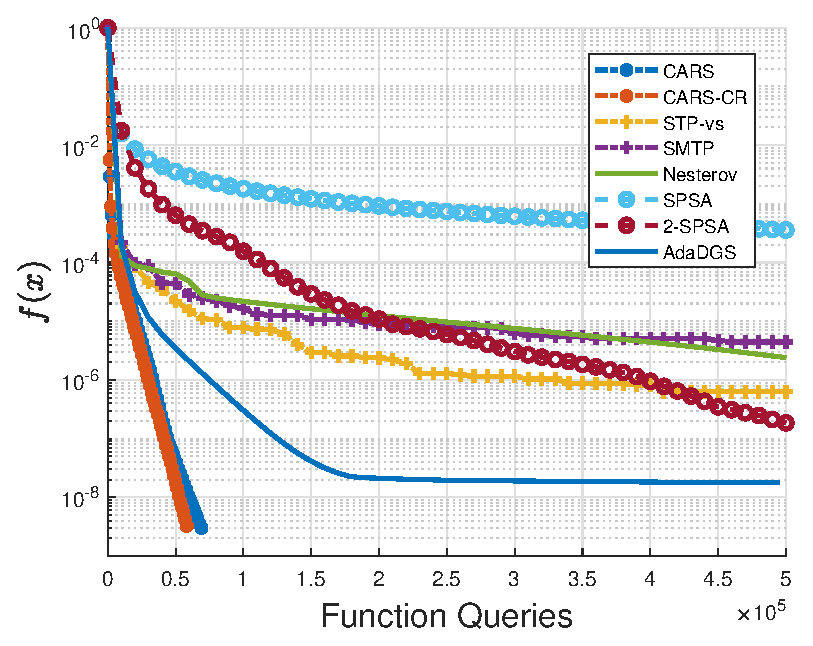
\includegraphics[width=0.8\linewidth]{Quartic_Noiseless_1e-09.eps}
    \caption{Performance of each algorithm on a convex quartic function $f(x) = 0.1\sum_{i=1}^{d} x_i^4 + \frac{1}{2}x^{\top}Ax + 0.01\|x\|^2$, where $A = G^{\top}G$ with $G_{ij} \stackrel{i.i.d}{\sim} \mathcal{N}(0, 1)$. The problem dimension $d = 30$.}
    \label{fig:Convex Quartic}
\end{figure}

\subsection{Benchmark Problem Sets with Non-Convex Functions}
The test results in this section are presented in the form of performance profiles \cite{dolan2002benchmarking}, which is a commonly used tool for comparing the performance of multiple algorithms over a suite of test problems. Performance profiles tend to be more informative than single-dimensional summaries ({\em e.g.} average number of iterations required to solve a problem). Formally, consider fixed sets of problems $\mathcal{P}$ and algorithms $\mathcal{S}$. For each $p \in \mathcal{P}$ and $s \in \mathcal{S}$ the {\em performance ratio} $r_{p,s}$ is defined by
\begin{equation*}
    r_{p,s} = \frac{t_{p,s}}{\min_{s'\in\mathcal{S}} t_{p,s'}},
\end{equation*}
where $t_{p,s}$ is the number of function queries required for $s$ to solve $p$. This is the relative performance of $s$ on $p$ compared to the best algorithm in $\mathcal{S}$ for $p$. The {\em performance profile} of $s$, $\rho_{s} : [1,\infty) \rightarrow [0,1]$ is defined as
\begin{align*}
    \rho_s(\tau) = \frac{|\{p \in \mathcal{P} : r_{p,s} \leq \tau \}|}{|\mathcal{P}|}.
\end{align*}
Therefore, $\rho_s(1)$ is the fraction of problems for which $s$ performs the best, while $\rho_s(\tau)$ for large $\tau$ measures the robustness of $s$. For all $\tau$, a {\em higher value of $\rho_{s}(\tau)$ is better}. We use a log-scale on the horizontal access when plotting $\rho_s(\tau)$.

%\paragraph{Mor\'{e}-Garbow-Hillstrom Problems.}
\vspace{0.1in}
\noindent\textit{\textbf{Mor\'{e}-Garbow-Hillstrom Problems.}}\quad
We tested the same set of algorithms using the well-known non-convex Mor\'{e}-Garbow-Hillstrom 34 test problems \cite{more1981testing}.
For each target accuracy $\varepsilon$, a problem is considered solved when we have $f(x_k)-f_\star \leq \varepsilon(f(x_0)-f_{\star})$ within the budget of 20,000 queries. We used the recommended starting point $x_0$ as in \cite{more1981testing} for all the tested algorithm, and repeated each test 10 times. The results are presented in Figure~\ref{fig:More Garbow Hillstrom and CUTEst}.

%\paragraph{CUTEst Problems.}
\vspace{0.1in}
\noindent\textit{\textbf{CUTEst Problems.}}\quad
We further assessed the performance of CARS and CARS-CR to the same suite of algorithms on the CUTEst \cite{gould2015cutest} problem set, which contains various convex and non-convex problems.
As before, we compared the methods using performance profiles for the 146 problems with dimension less than or equal to 50. The query budget for each problem was set to be $20,000$ times the problem dimension. The target accuracies were again set to $\varepsilon (f(x_0) - f_\star)$. The results are reported in Figure~\ref{fig:More Garbow Hillstrom and CUTEst}.


\begin{figure}
    \centering
    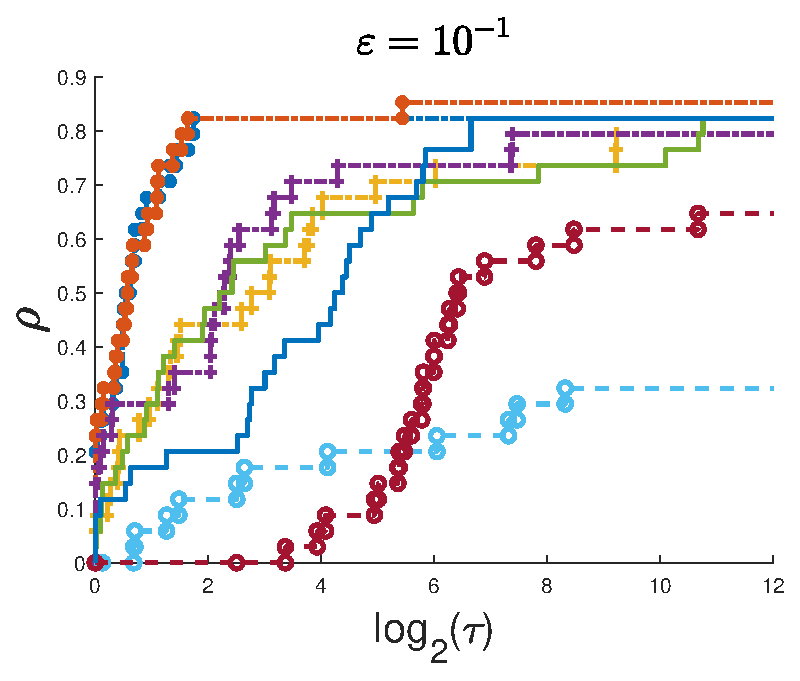
\includegraphics[width=0.4\linewidth]{MORE_perf_prof_1e-01_09-Mar-2023.eps}\qquad
    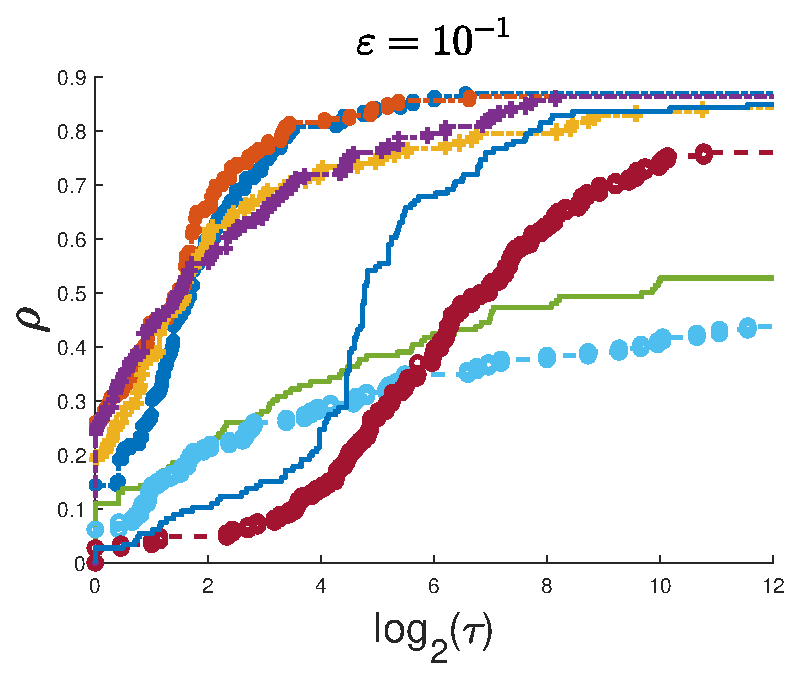
\includegraphics[width=0.4\linewidth]{CUTEst_perf_prof_1e-01_08-Mar-2023.eps} \\
    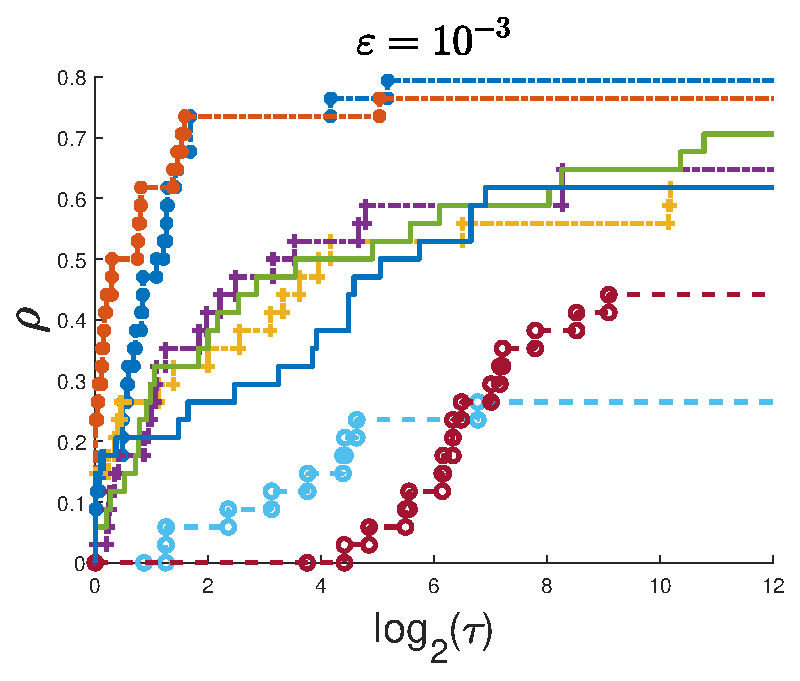
\includegraphics[width=0.4\linewidth]{MORE_perf_prof_1e-03_09-Mar-2023.eps}\qquad
    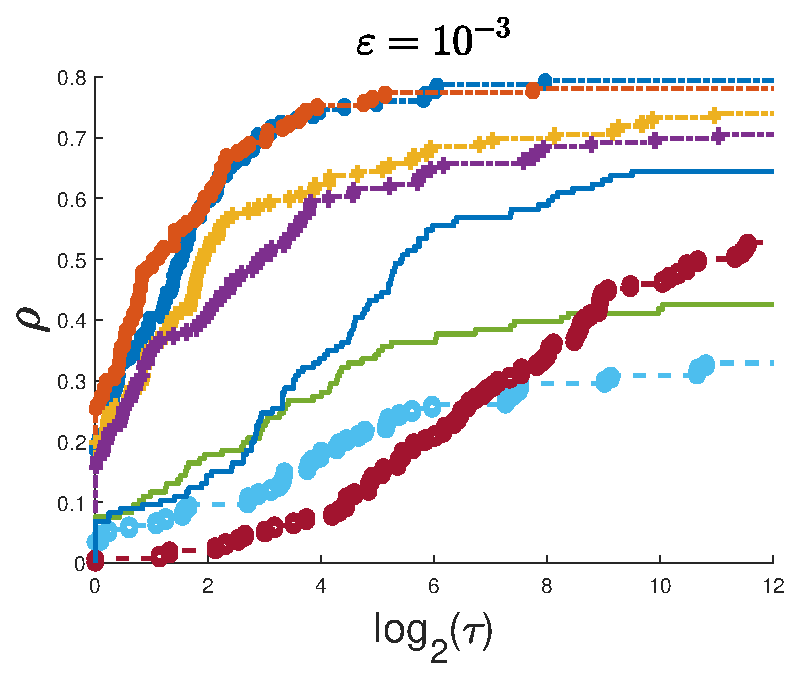
\includegraphics[width=0.4\linewidth]{CUTEst_perf_prof_1e-03_08-Mar-2023.eps} \\
    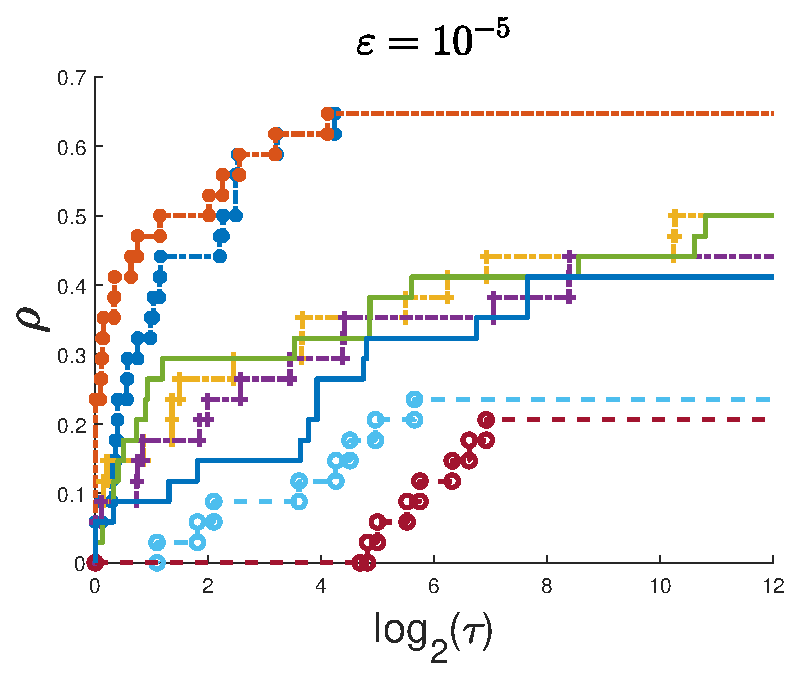
\includegraphics[width=0.4\linewidth]{MORE_perf_prof_1e-05_09-Mar-2023.eps}\qquad
    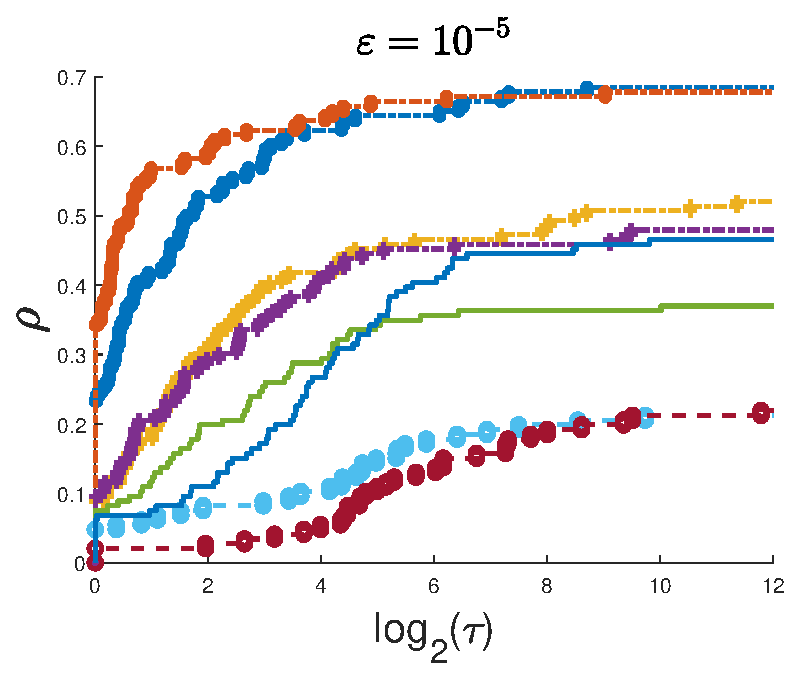
\includegraphics[width=0.4\linewidth]{CUTEst_perf_prof_1e-05_08-Mar-2023.eps}
    \\
    \vspace{5mm}
    {
        \setlength{\fboxsep}{0pt}
        \fbox{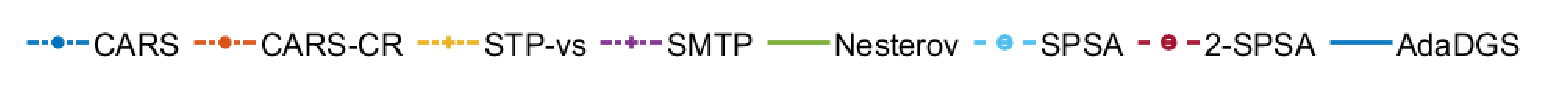
\includegraphics[width=0.8\linewidth]{legend_MORE_all.eps}}
    }\caption{Performance profiles on Mor{\'e}-Garbow-Hillstrom problems (\textbf{left}) and CUTEst problems (\textbf{right}), for various target accuracies $\varepsilon = 10^{-1}$ (\textbf{top}), $10^{-3}$ (\textbf{middle}), and $10^{-5}$ (\textbf{bottom}). Our results demonstrate that CARS and CARS-CR consistently outperform other methods in terms of both efficiency ($\rho$ at low $\tau$ values) and robustness ($\rho$ at high $\tau$ values.) at all levels of accuracy.}\label{fig:More Garbow Hillstrom and CUTEst}
\end{figure}

\subsection{Problems with Highly Oscillatory Noise}
We also evaluated the performance of the algorithms, including CARS-NQ, on the same set of problems, but this time with additional highly oscillatory noise. The results are depicted in Figure~\ref{fig:Convex Quartic with Noise}.
The experiment notably showcases the efficacy of an increased sampling radius for CARS-NQ.
\begin{figure}
    \centering
    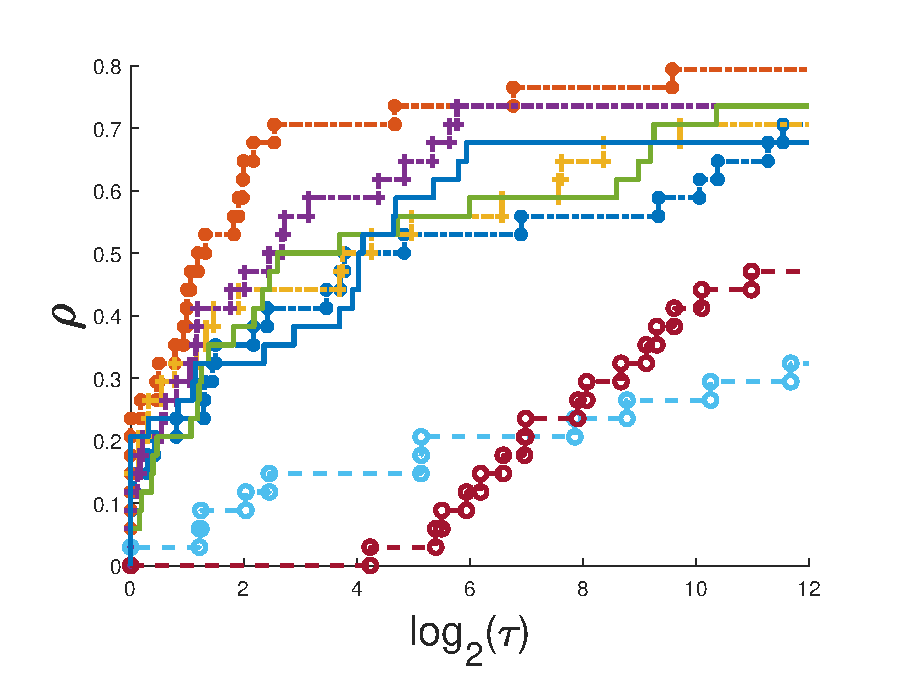
\includegraphics[width=0.8\linewidth]{Osc_MORE_ALL_EPS_1e-3_noise_0.05EPS.eps}
    \vspace{1mm}
    {
        {\includegraphics[width=0.8\linewidth]{MORE_ALL_LEGEND.png}}
    }
    \caption{Performance of each algorithm on Mor\'{e}-Garbow-Hillstrom Problems with sinusoidal noise $f_{\mathrm{osc}}(x) = \psi \frac{1}{d}\sum_{i=1}^{d}(1-\cos(\phi x_i))$, where  $\psi = 0.05\varepsilon(f(x_0)-f_\star)$ and $\phi = 100\pi$. The target accuracy $\varepsilon$ is set to $10^{-3}$.}
    \label{fig:Convex Quartic with Noise}
\end{figure}



\subsection{Black-box Adversarial Attacks}
\begin{table}[t]
    \centering
    \def\ROWCOLOR{black!10!white}
    \begin{tabular}{l c c c}
        \toprule
        Algorithm      & Success Rate (\%) & Median Queries & Average Queries \\
        \midrule
        \rowcolor{\ROWCOLOR}
        ZOO$^*$        & 93.95             & 11,700         & 11,804          \\
        PGD-NES$^*$    & 88.39             & 2,450          & 4,584           \\
        \rowcolor{\ROWCOLOR}
        ZOHA-Gauss$^*$ & 91.69             & 1,400          & 2,586           \\
        ZOHA-Diag$^*$  & 91.06             & 1,656          & 3,233           \\
        \rowcolor{\ROWCOLOR}
        STP            & 53.64             & 2,193          & 3,141           \\
        SMTP           & 65.68             & 1,415          & 2,250           \\
        \rowcolor{\ROWCOLOR}
        Nesterov       & 67.72             & 1,105          & 2,044           \\
        Square Attack  & \textbf{98.21}   & 1,060          & 1,297           \\
        \rowcolor{\ROWCOLOR}
        CARS (Square)  & 97.09             & \textbf{717}  & \textbf{1,169} \\
        \bottomrule
    \end{tabular}
    \caption{Comparison of success rates, and median and average function queries for the successful black-box adversarial attacks on MNIST with $\ell_\infty$-perturbation bound 0.2.
        CARS, equipped with the Square Attack's distribution, shows the best performance in successful attacks, while reaching the second best success rate. The results marked with $^*$ are cited from \cite{ye2018hessian}.
    }
    \label{table: Black Box Attack to a CNN model on the MNIST dataset}
\end{table}
Suppose $\mathcal{N}$ is an image classifier.
The problem of generating small perturbations $x$ that, when added to a natural image $x_{\mathrm{nat}}$, fool the classifier ({\em i.e.} $\mathcal{N}(x_{\mathrm{nat}} + x) \neq \mathcal{N}(x_{\mathrm{nat}})$) is known as finding an {\em adversarial attack} \cite{goodfellow2014explaining}. As described in \cite{chen2017zoo}, when no access to the internal workings of the classifier
is available, this problem becomes a black-box, or derivative-free, optimization problem. In order to ensure the attacked image $x_{\mathrm{nat}} + x$ appears natural, a pixel-wise bound $\|x\|_{\infty} \leq \varepsilon_{\mathrm{atk}}$ is usually enforced. CARS showed state-of-the-art performance in generating black-box adversarial attacks for $\mathcal{N}$ trained on the MNIST digit classification dataset \cite{lecun2010mnist}.

In our experiments, $\mathcal{N}$ is a two-layer CNN achieving $99\%$ test accuracy on unperturbed images. We use $\varepsilon_{\mathrm{atk}} = 0.2$ and consider all $10,000$ images from the test set of MNIST. We consider an attack a success if it fools $\mathcal{N}$ before a budget of $10,000$ queries is met. The success rates, median and average queries for successful attacks are shown in Table~\ref{table: Black Box Attack to a CNN model on the MNIST dataset}.
The results from ZOO \cite{chen2017zoo}, PGD-NES \cite{ilyas2018black}, and ZOHA-type algorithms \cite{ye2018hessian} are cited from \cite{ye2018hessian}.
As pointed out in Section~\ref{section:convergence of CARS}, the choice of sampling directions for CARS is not restrictive. Hence we used a similar initialization and distribution $\mathcal{D}$ as the Square Attack \cite{andriushchenko2020square}, which is known to be particularly well-suited for attacking CNN models.
Visualization of attacked images is partly shown in Figure~\ref{fig:MNIST_ATK_RES}. More pictures and detailed settings can be found in Appendix~\ref{appendix: Experiments}.

\begin{figure}
    \centering
    \includegraphics[width=0.8\linewidth]{MNISTatk_imgs_horizontal_60_B.eps}
    \caption{Adversarial examples with misclassified labels on MNIST generated with CARS. More pictures are available in Appendix~\ref{appendix: Experiments}.}
    \label{fig:MNIST_ATK_RES}
\end{figure}

\subsection{Benchmarking the Performance of SHIPS}
In this section we present a numerical result for SHIPS, which is a combination of CARS and the randomized matrix inversion presented in Section~\ref{section:SHIPS}. The main purpose of this comparison is to assess SHIPS' ability to generate effective search directions. Thus, we contrast it with Exact Gradient Descent (Exact GD), and variance-reduced version of CARS and Nesterov-Spokoiny (CARS-VarRed and NS-VarRed, respectively.) 

For a fairer comparison with methods based on exact derivatives, we, in the case of DFO methods, sample $d$ directions and use $2d$ queries to estimate the directional derivatives per iteration.

Variance reduction, achieved by utilizing multiple samples when calculating the expectation, has shown to work well for Nesterov-Spokoiny \cite{salimans2017evolution,mania2018simple}.
In contrast, CARS, does not have a known reduced variance version yet. For this, we apply a multi-sample extension \eqref{eq: ES extension of CARS multiple samples} as introduced in Section~\ref{section: connection to ES}.

The test function for our benchmark is given by:
\begin{equation}
    f(x) = \frac{1}{2}x^{\top}A x + \frac{1}{12} \sum_{i=1}^{d} \alpha_{i} x_{i}^{4},
\end{equation}
where $A$ is a random positive definite matrix with $A = G^{\top}G$ with $G_{ij} \stackrel{i.i.d}{\sim} \mathcal{N}(0, 1)$, and $\alpha_i \stackrel{i.i.d}{\sim} \unif(0, 1)$.

For each iteration, we used $d$ uniformly random directions on the unit sphere, and consumed $2d$ queries to estimate the respective directional derivatives. 
The methods labeled \emph{Exact GD} and \emph{Exact SHIPS} are provided with the exact gradient and Hessian for comparative purposes.
As demonstrated in Figure~\ref{fig:SHIPS_vs_others}, SHIPS deivers superior convergence speed.

\begin{figure}
    \centering
    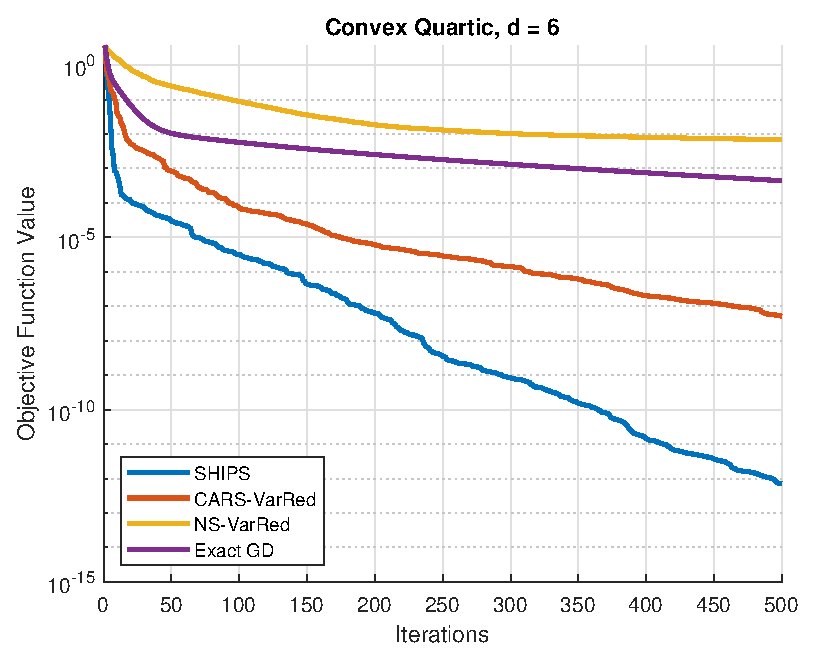
\includegraphics[width=0.8\linewidth]{SHIPS_vs_others.eps}
    \caption{The $x$-axis denotes the number of iterations, not the number of function queries. Among all the methods, SHIPS shows the best convergence rate,  outperforming even Exact GD, as it effectively utilizes the curvature information.}
    \label{fig:SHIPS_vs_others}
\end{figure}



\chapter{Bridging the Gap Between Local and Global DFO Method Through Inspection Strategy}
\label{Chapter: Insepction}

% Introduction
\section{Introduction}
In this chapter, we discuss the inspection strategy for DFO methods, focusing on filling the significant gap between global and local optimization strategies.

When the objective function is non-convex and has spurious local minima, it is in general difficult to find the global minimum using local optimization methods.
Global optimization methods
In such cases, local optimization methods are often used to find a local minimum. However, the quality of the local minimum is not guaranteed, and it is often difficult to quantify how good the solution is.
Global optimization methods seek the absolute best solution throughout the entire solution space. While this ensures the optimal solution is found, these methods can be computationally intensive, particularly for high-dimensional problems. On the contrary, local optimization methods are geared towards finding a suitable solution within a localized area of the solution space. Although efficient, these methods may overlook the global optimum if it is located outside a certain neighborhood.

We delve into the dichotomy between these two optimization strategies and discuss the $R$-local optimization approach \cite{chen2019run}, designed to bridge this gap. $R$-local optima lie between local and global optima, and often ensures a satisfactory solution quality by providing a definable radius for the solution's local neighborhood.

We also explore how $R$-local optimization interacts with DFO methods. Despite their advantages, $R$-local optimization methods can be computationally expensive, particularly when the cost of sampling the objective function is not significantly cheaper than the gradient. However, in the context of DFO, the addition of inspections may not substantially impact the overall sample complexity.

Our proposed framework directs local DFO methods towards an $R$-local minimum using a similar number of additional queries, up to a constant factor, to those the method would typically consume \emph{per iteration}. This algorithm that doesn't rely on a global surrogate model, which can be computationally demanding in high-dimensional scenarios.


\subsection{The gap between global optimization and local optimization}
The majority of the optimization methods are either global optimization or local optimization methods. They approach these problems in very different ways, which creates a gap between them. 

\paragraph{Global Optimization} This class of methods aims to find the absolute best solution (up to a small tolerance) in the \emph{entire} solution space for an optimization problem. In other words, it searches for the overall minimum or maximum. The techniques used for global optimization are typically exhaustive, as they have to explore the entire problem space to ensure they have found the best possible solution up to the tolerance. This is because there may be many local optima, but only one (or a few) global optima. As a result, these methods can be computationally expensive, particularly for complex, high-dimensional problems.

\paragraph{Local Optimization} This class of methods, on the other hand, focuses on finding a good solution in a neighborhood, no matter how small it is, of a specific point in the solution space. This does not necessarily mean that the solution will be the best overall; instead, it means that there is no better solution in some vicinity of the found one. Thus, local optimization methods can be faster and less computationally expensive than global ones, but they may miss the global optimum if it lies outside of the selected neighborhood.

\paragraph{Gap between these two types of optimization} The gap can be understood through the following perspectives.

Global optimization guarantees the best solution, while local optimization only guarantees the best solution within a local neighborhood. However, the size of the neighborhood is not known or controllable.

Due to the need to explore the entire solution space, global optimization usually requires much more computational effort, causing much longer running time, than local optimization.

In practice, the choice between local and global optimization often depends on the specific problem, the resources available, and the acceptable trade-offs. For low-dimensional problems where it is crucial to find the absolute best solution, global optimization becomes necessary. However, for many problems, a solution that is ``good enough'' is sufficient. 

Local methods, despite only producing local solutions, may be preferred and sometimes are only the choice due to their efficiency. 
To improve the solution quality of local methods, meta-heuristics were introduced. They include using multiple starting points, simulated annealing, genetic algorithms that allow occasional moves in the worse direction, etc.
However, neither local methods nor their meta-heuristic improvements could quantify how ``good enough'' their solutions are.

\paragraph{Filling the gap by $R$-local optimization}
According to \cite{chen2019run}, 
an $R$-local minimizer is a type of local minimizer that specifies a radius of the local neighborhood around the minimizer.

More specifically, suppose we would like to minimize a function $f: \mathbb{R}^n \rightarrow \mathbb{R}$. We say that $x^\star\in\mathbb{R}^n$ is an $R$-local minimizer of $f$ if  that $x^\star$ is a  minimizer of $f$ in the closed ball ${x \in \mathbb{R}^n: \|x - x^\star\| \leq R}$.
This means $x^\star$ is a local minimizer in the neighborhood of radius $R$ around it. 

The concept of an $R$-local minimizer is often used when we want to guarantee the solution found to have a sufficient quality in a vicinity of a defined size. This can be helpful when the global minimizer cannot be easily found or when the function is too complex to optimize over its entire domain. The value of $R$ could be chosen based on some prior knowledge or through a process of trial and error.

\subsection{DFO and \$R\$-local optimization}
$R$-local optimization offers clear advantages over purely local methods in terms of discovering better solutions. However, it often incurs a higher computational cost, specifically requiring \BK{$\mathcal{O}(s \exp({O(d')}))$ samples for $s$ blocks of dimension $d'$ as shown in \cite{chen2019run}}.
This can become prohibitively expensive in certain scenarios\BK{, particularly when the cost of sampling the objective function and its gradient is approximately equal}. However, in derivative-free optimization, unless there are special structures (such as sparse gradients described in \cite{cai2020zeroth}), an additional factor of $d$, compared to its gradient-based counterpart, in the sample complexity is unavoidable. Consequently, performing inspections may not significantly impact the overall sample complexity, but only up to a constant factor.



% Main Results

\section{Main Results}
Suppose that we have a local DFO method (e.g. Nesterov-Spokoiny\cite{nesterov2017random}, or CARS\cite{kim2021curvature}) that consumes up to $\mathcal{O}(d^\nu)$ queries per iteration. (for instance, $\nu = 0$ for CARS, and $\nu=1$ for AdaDGS. For Nesterov-Spokoiny, $\nu$ is typically 0 or 1, depending on the level of approximation to the Monte-Carlo approximation).
The main idea is to use additional queries, up to the same $\mathcal{O}(d^\nu)$, to drive the method to converge to an $R$-local minima with high probability. The resulting algorithm thus requires the same order of magnitude in terms of function queries.
In addition to that, we want it to be a model-free algorithm, meaning that we don't set up a global surrogate model for the problem, which is often quite expensive when $d$ is large.



\begin{definition}[Successful Inspection] Given a descent threshold $\nu$, an inspection at a point $y$ around $x$ is said to be successful $\nu \geq 0$ if $f(y) < f(x) - \nu$.
\end{definition}


\begin{algorithm}[H]
\caption{Inspect as You Run}
 \label{alg:IR general}
\begin{algorithmic}[1]
  \State \textbf{Input:} $x_0$: initial point; $r$: sampling radius; $R$: inspection radius; $\mathcal{A}$: One step of a DFO method, generating the next iterate; $n_k$: maximum number of inspections at $k$-th iteration; $\nu$: descent threshold
  \State Get the oracle $f(x_0)$.
  \For{$k = 1, \cdots, K$}
        \State Compute $x_{k, 0} = \mathcal{A}(x_k)$
        \For {$j = 1, \cdots, n_k$}
            \State Compute $f(x_{k,j})$ 
            \If{$f(x_{k,j}) < f(x_{k,0}) - \nu$}
                \State Set $x_{k+1} = x_{k,j}$ and \emph{break}
            \EndIf
        \EndFor
        \State If no successful inspections, set $x_{k+1} = x_{k,0}$ \label{eq: inspection step in the algorithm 1}
  \EndFor
   \State \textbf{Output:} $x_K$: estimated optimum point.
\end{algorithmic}
\end{algorithm}

\subsection{Analysis}
% In this section we largely depend on the analysis in \cite{chen2019run} to guarantee the convergence of this plug-in algorithm to an appropriate point.
% First we introduce a blockwise $\mathbf{R}$-local minimizer, which generalizes the $R$-local minimizer.

% Cite Run-and-Inspection paper's results

% When $f$ has a form $g + \rho$, where $g$ has $L$-Lipschitz gradient and is Polyak-{\L}ojasiewicz (PL), and $\rho$ satisfies:
% \begin{align*}
%     |\rho(x)- \rho(y)| \leq \alpha \|x-y\| + 2\beta ,
% \end{align*}
In this section, we provide an analysis for the point obtained from Algorithm~\ref{alg:IR general}.
Roughly speaking, if the recent $M$ inspections did not give a better point than the local DFO method $\mathcal{A}$, it is an $R_0$-local minimum with probability at least $1 - \exp(-\mathcal{O}(M))$, for some $R_0 < R$.

We assume the objective function $f$ satisfies the conditions for the DFO method $\mathcal{A}$ to converge. In addition, we also assume $f$ is $\bar{L}$-Lipschitz continuous. Note that, however, if $\nabla f$ is already assumed to be Lipschitz, like in the analyses of many methods, the assumption implies the Lipschitz continuity of $f$.

% Although a local DFO method that estimates the derivatives by finite difference can smooths out the effect of $\beta$ with large sampling radius $r$, they also blow up if $r$ is too small. Thus we assume $\beta= 0$ here for a simpler analysis.
% In practice, one can use an appropriate lower bound for $r$ to achieve an approximate optimum.
% thus  for instance, $O(\varepsilon^{1/4})$ for CARS 

% Theorem 5 in \cite{chen2019run} gives a sufficient condition for a $\mathbf{R}$-local minimizer $\bar{x}$ being an approximate global minimizer. Furthermore, Theorem 7 states that an \emph{approximate} $\mathbf{R}$-local minimizer can also be one. Finally, Theorem 9 addresses the condition to guarantee an approximate $\mathbf{R}$-local minimizer.



For CARS \cite{kim2021curvature}, for instance, it originally uses 4 (CARS, the vanilla version) or 5 (CARS-CR) queries per iteration. Thus by adding, for instance, 3 queries for inspection per iteration, we have the IR version of CARS, whose cost is up to 75\% more than the original method per iteration.

In particular, for convex problems the overall cost will be increased with at most a constant factor. However, we argue that with inspection one can find significantly better local minima for a certain class of nonconvex problems.

\begin{theorem} \label{thm: high prob guarantee of an approx. R-local min}
    Let $\{x_k\}_{k=1}^{K}$ be the sequence of points obtained from Algorithm~\ref{alg:IR general}. Assume that no successful inspections occur for all $k \geq k_0$, and let $m$ be the total number of inspections for $k \geq k_0$. Suppose
    \begin{align*}
        \|x_{k} - x_K\| \leq D < R \quad \text{for all } k \geq k_0.
    \end{align*}
    Define $R_0 = R-D$ and choose a positive $\tilde{r} < D$. Then, $x_K$ is an $R_0$-local minimum up to $\eta = \bar{L}\tilde{r} + \nu$ with probability at least $1-\exp(- m (\tilde{r}/R)^d)$.
\end{theorem}
\begin{proof}
    Begin by noting that the ball $B(x_K, R_0 + \tilde{r})$ is a subset of $B(x_{k}, R)$ for all $k \geq k_0$. Hence, for a random variable $z \sim \mathrm{Unif}(B(x_{k}, R))$, the conditioned random variable $z|\mathcal{A}$, where $\mathcal{A}$ is the event $z \in B(x_K, R_0 + \tilde{r})$, follows the uniform distribution over $B(x_K, R_0 + \tilde{r})$.

    At iteration $k= K$, define $S = \{y_i\}_{i=1}^{M}$ as the subset of the recent $m$ inspection points contained within $B(x_K, R_0 + \tilde{r})$. Then $M$ follows the binomial distribution $M \sim \mathrm{Binomial}( m , \phi_1)$ with $\phi_1 = \left(\frac{R_0  + \tilde{r}}{R}\right)^d$.
    
    We now demonstrate that if $S$ is sufficiently dense, $x_K$ becomes an approximate $R_0$-local minimum. Consider
    \begin{align*}
        \tilde{x} := \argmin_{x \in B(x_K, R_0)} f(x).
    \end{align*}
    If there exists $y_i \in S \cap B(\tilde{x},\tilde{r})$, knowing $y_i$ is not a successful inspection, we obtain 
    \begin{align*}
        f(x_K) \leq f(\tilde{x}) + (f(y_i) - f(\tilde{x})) + \nu
        \leq \min_{x \in B(x_K, R_0)}f(x) + \bar{L} \tilde{r} + \nu,
    \end{align*}
    implying that $x_K$ is an $R_0$-local minimum up to $\eta = \bar{L}\tilde{r} + \nu$.
    
    Finally, we need to find the probability bound for $S \cap B(\tilde{x}, \tilde{r})$ not being empty. As each $y_j \sim \mathrm{Unif}(B(x_K, R_0 + \tilde{r}))$ and $B(\tilde{x},\tilde{r}) \subseteq B(x_K, R_0 + \tilde{r})$, we get $\phi_2 := \mathbb{P}[y_j \in B(\tilde{x}, \tilde{r})] = \left(\frac{\tilde{r}}{R_0 + \tilde{r}}\right)^d$. Consequently,
    \begin{align*}
        & \quad~\mathbb{P}[y_j \not\in B(\tilde{x}, \tilde{r}) \text{ for all } j = 1, \cdots, M] \\
        & =\sum_{M' = 0}^{\infty} \left(1 - \phi_2\right)^{M'} \mathbb{P}[M = M'] \\
        & =\mathbb{E}_{M}(\exp{(M\log(1-\phi_2))}) \\
        & \stackrel{(a)}{=} (1-\phi_1 + \phi_1 \exp{(\log(1-\phi_2))})^m \\
        & = (1-\phi_1 \phi_2 )^m \\
        & \leq \exp(-m\phi_1 \phi_2), & \text{($1-x \leq \exp(-x)$)}
    \end{align*}
    where (a) is from the moment generating function formula for binomial distributions.
    And since $\phi_1 \phi_2 = (\tilde{r}/R)^d$, $S \cap B(\tilde{x}, \tilde{r})$ is nonempty with a probability of at least $1 - \exp(-m (\tilde{r}/R)^d)$.
\end{proof}



Theorem~\ref{thm: high prob guarantee of an approx. R-local min} states that when we are near the local minimum found by a DFO method, we can guarantee, with probability $1-\delta$, it is indeed an approximate $R_0$-local minimum with a total number of $\log(\delta^{-1}) \left(\frac{R}{\tilde{r}}\right)^d$ inspections.


% Numerical Experiments
\section{Experimental Results}
In this section we present the experimental results for supporting the effectiveness of inspection strategy for improving the solution quality of local DFO methods. As discussed in the previous section, we also provide the comparison between the local method equipped with inspection strategy and a global method, to emphasize the ease of problem structure exploitation.

Except for the last experiment, we benchmark a vanilla CARS and its IR version.

\subsection*{Spurious Local Minima}
We start with a simple quadratic function with added sinusoidal noise. An 1-D illustration is shown in Figure~\ref{fig: 1D quad + sin}.
This function has spurious local minima, whose number grows exponentially with the problem dimension $d$.
\begin{equation*}
    f(x) =  \sum_{i=1}^{d} \left((x_i)^2 + 0.2 \sin\left(10\pi(x_i - \frac{1}{20})\right) + 0.2 \right)
\end{equation*}
\begin{figure*}
    \centering
    {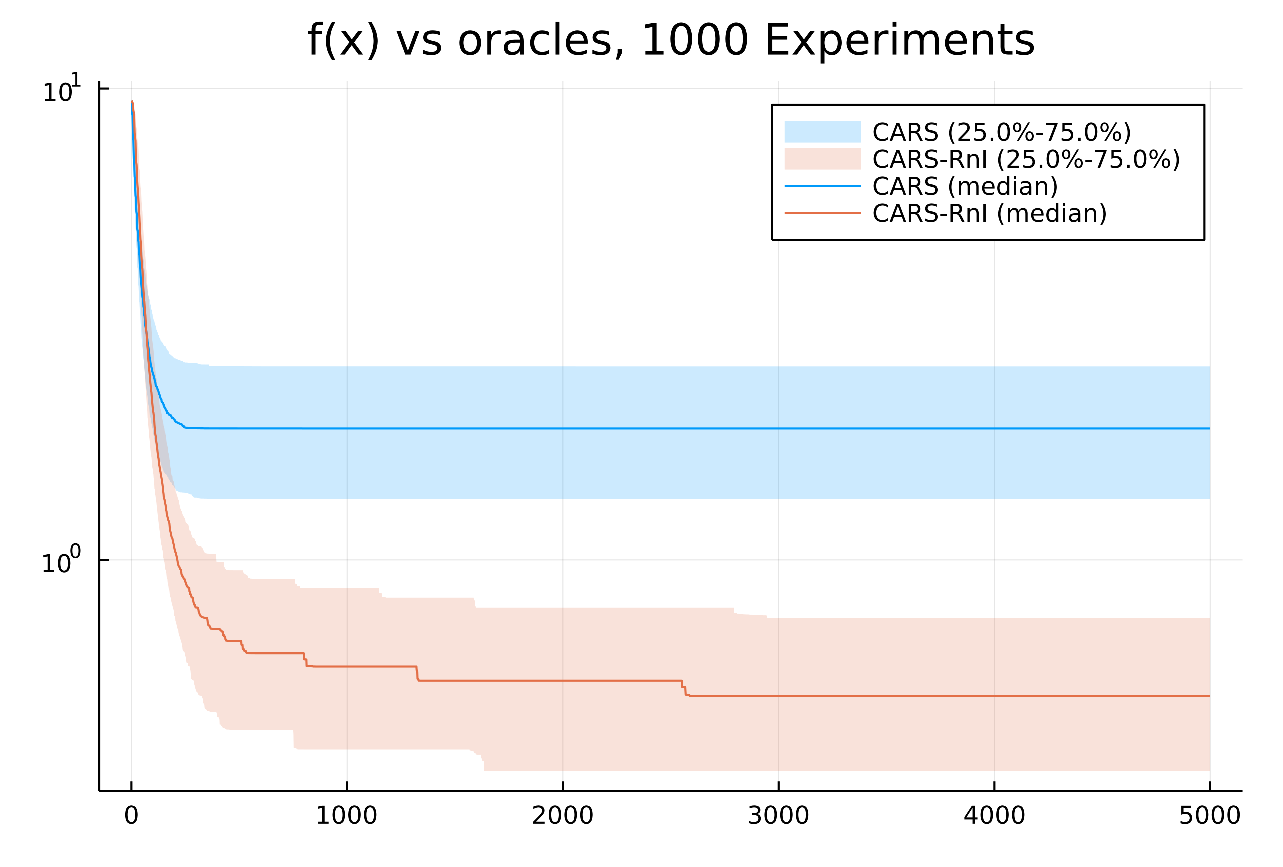
\includegraphics[width=0.7\linewidth]{freq10_amp0.2_quad_plus_sin.eps}}\\
    \vspace{3mm}
    {\includegraphics[width=0.7\linewidth]{freq10_amp0.2_quad_plus_sin_sols.eps}}
    \caption{Comparison of CARS and the Inspect-as-Running version of CARS for the quadratic function with sinusoidal noise.}
    \label{fig:Convex plus sine}
\end{figure*}
As depicted in Figure~\ref{fig:Convex plus sine}, the inspection strategy consistently identifies superior local minima, often reaching the global minima in a relatively lower dimension of 6.
We will revisit this example with a substantially higher dimension ($d=300$) for the comparison with global methods.

\subsection*{Ackley's Functions}
Ackley's functions are well-known non-convex functions with numerous spurious local minima:
\begin{equation*}
    f(x) = -20 \exp\left(-0.2 \sqrt{\|x\|^2/d}\right) - \exp\left(\sum_{i=1}^{d}{\cos(2\pi x_i)/d}\right) + e + 20.
\end{equation*}
 \cite{chen2019run} also introduced an asymmetric variant:
 \begin{align*}
    f(x,y) = -20 \exp(-0.04(x^2+y^2)) - \exp(0.7(\sin(xy) + \sin y) + 0.2\sin(x^2)) + 20
 \end{align*}
We tested both functions and again, observed that the IR version consistently found better minima, while the vanilla CARS frequently got trapped in a non-global local minima.
\begin{figure*}
    \centering
    {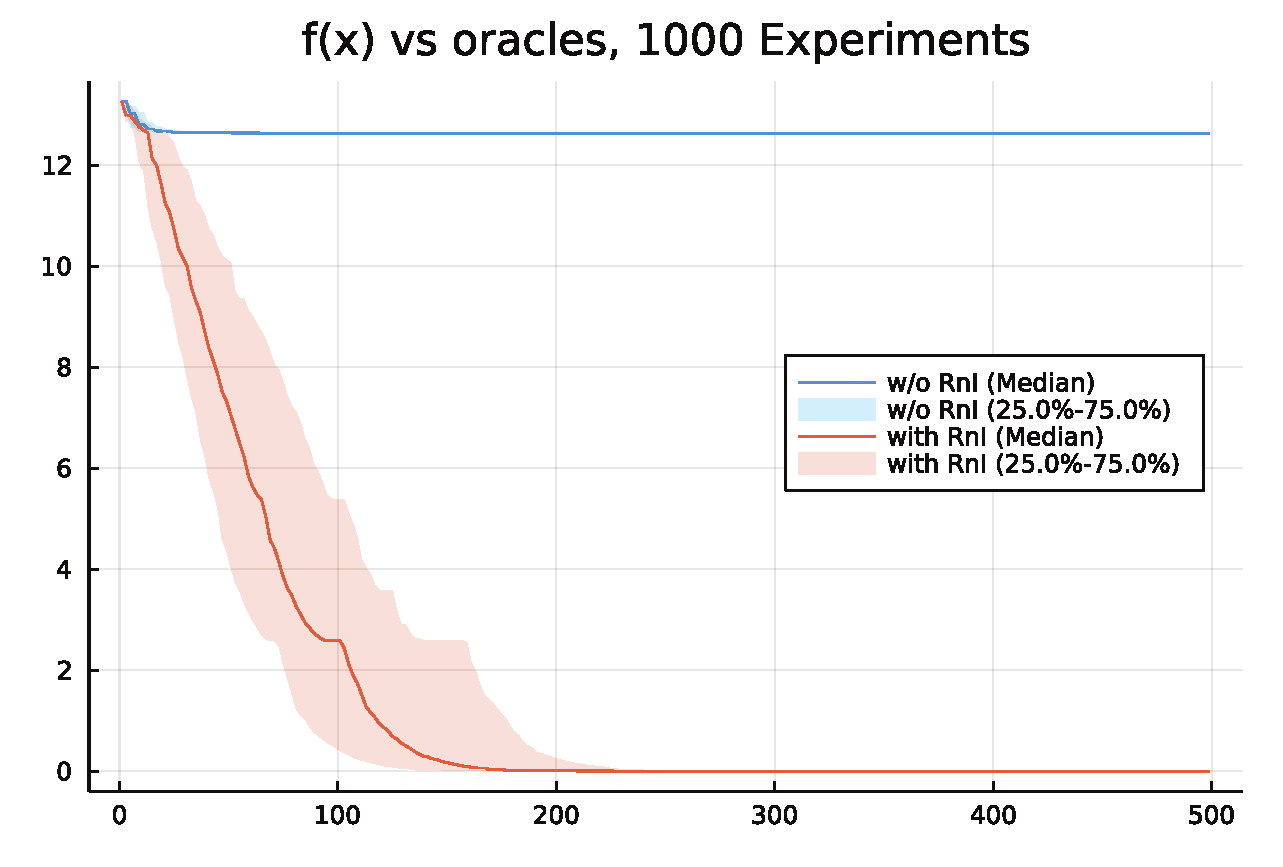
\includegraphics[width=0.7\linewidth]{Ackley.eps}}\\
    \vspace{3mm}
    {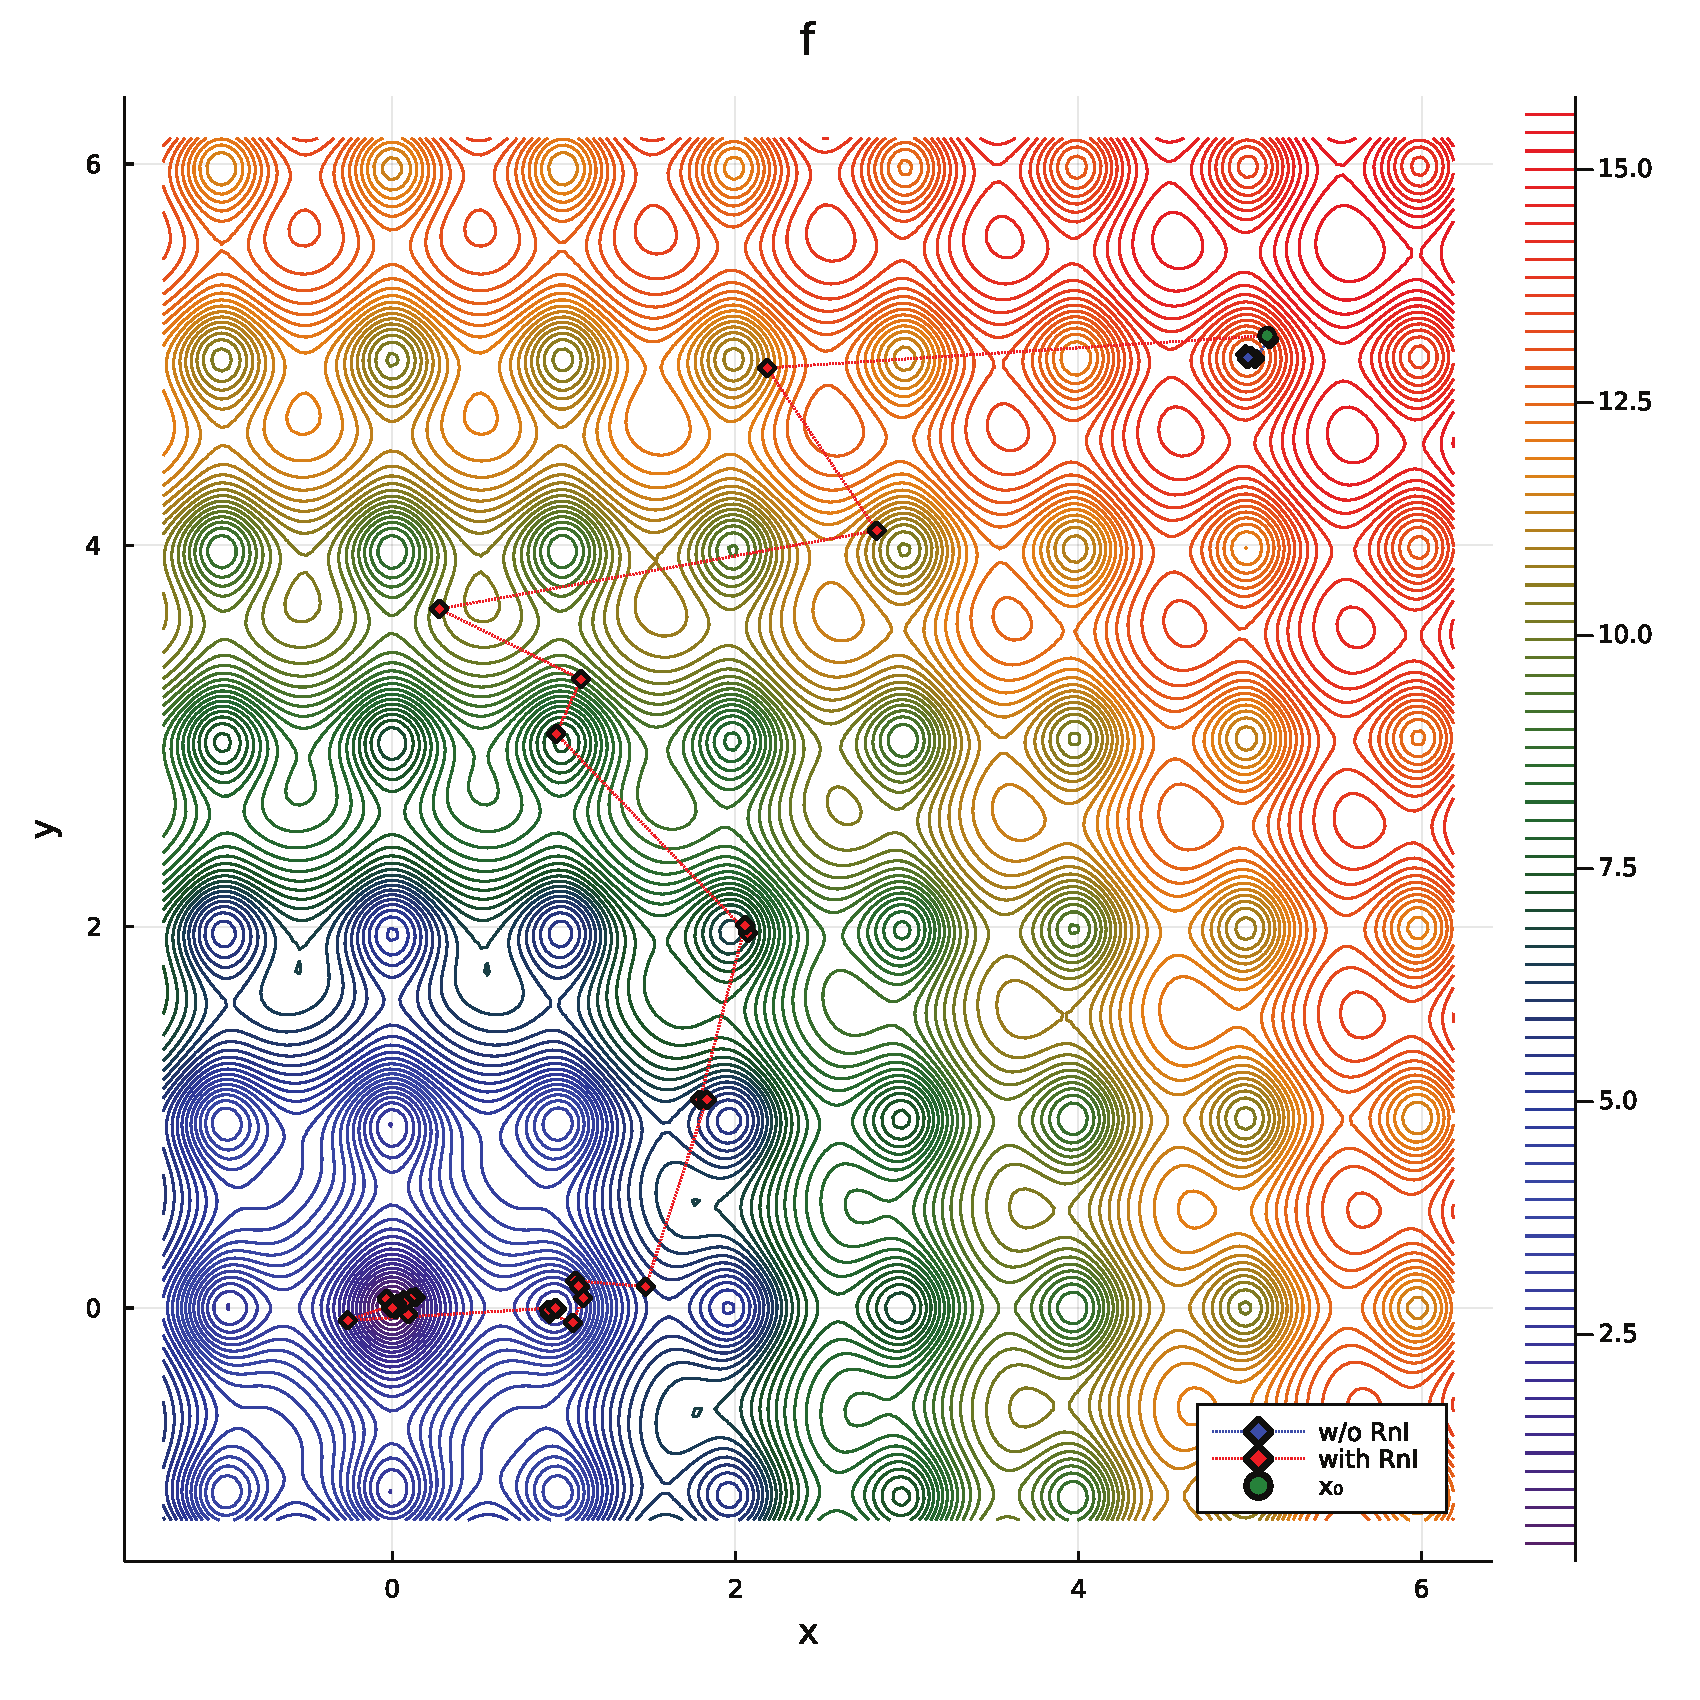
\includegraphics[width=0.7\linewidth]{Ackley_sols.eps}}
    \caption{Comparison of CARS and the Inspect-as-Running version of CARS for the Ackley function}
    \label{fig: Ackley}
\end{figure*}

\begin{figure*}
    \centering
    {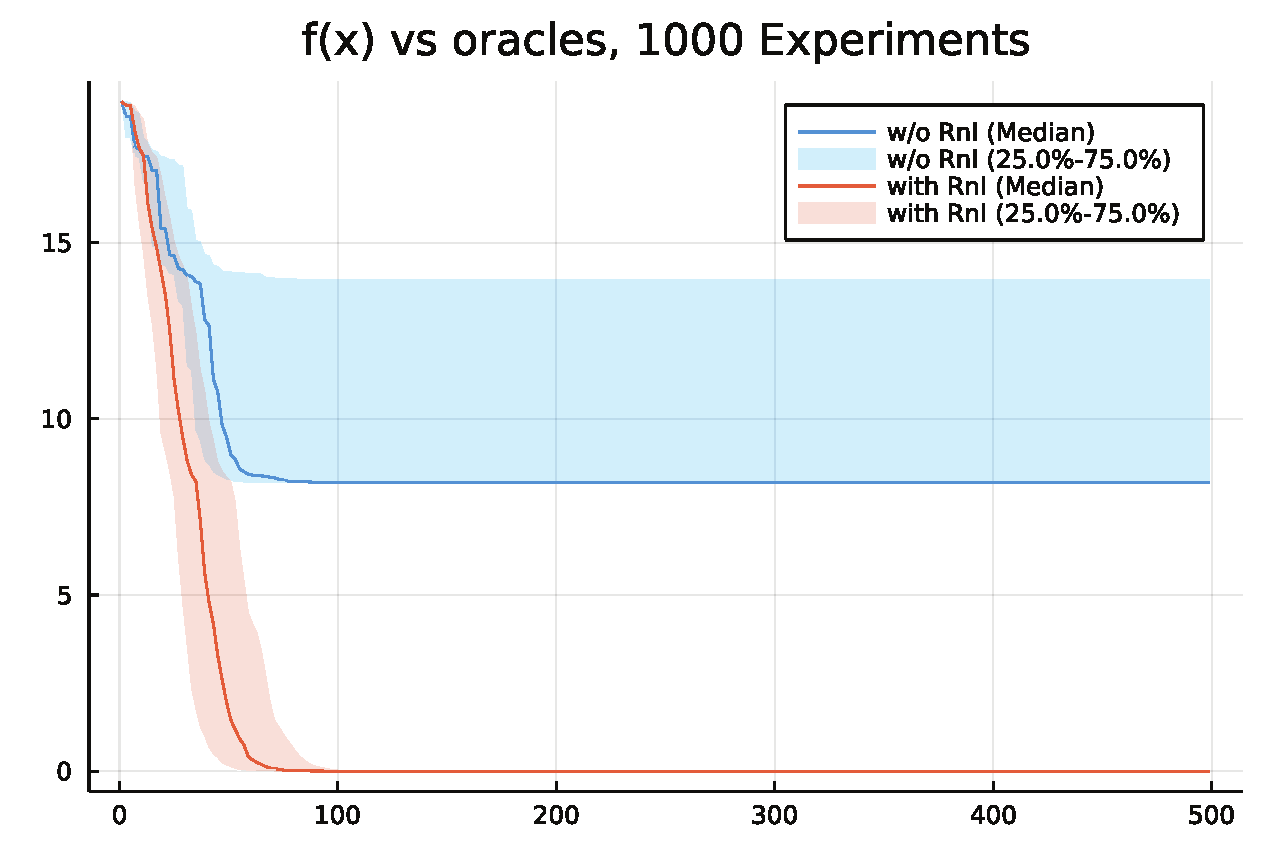
\includegraphics[width=0.7\linewidth]{asym_Ackley.eps}}\\
    \vspace{3mm}
    {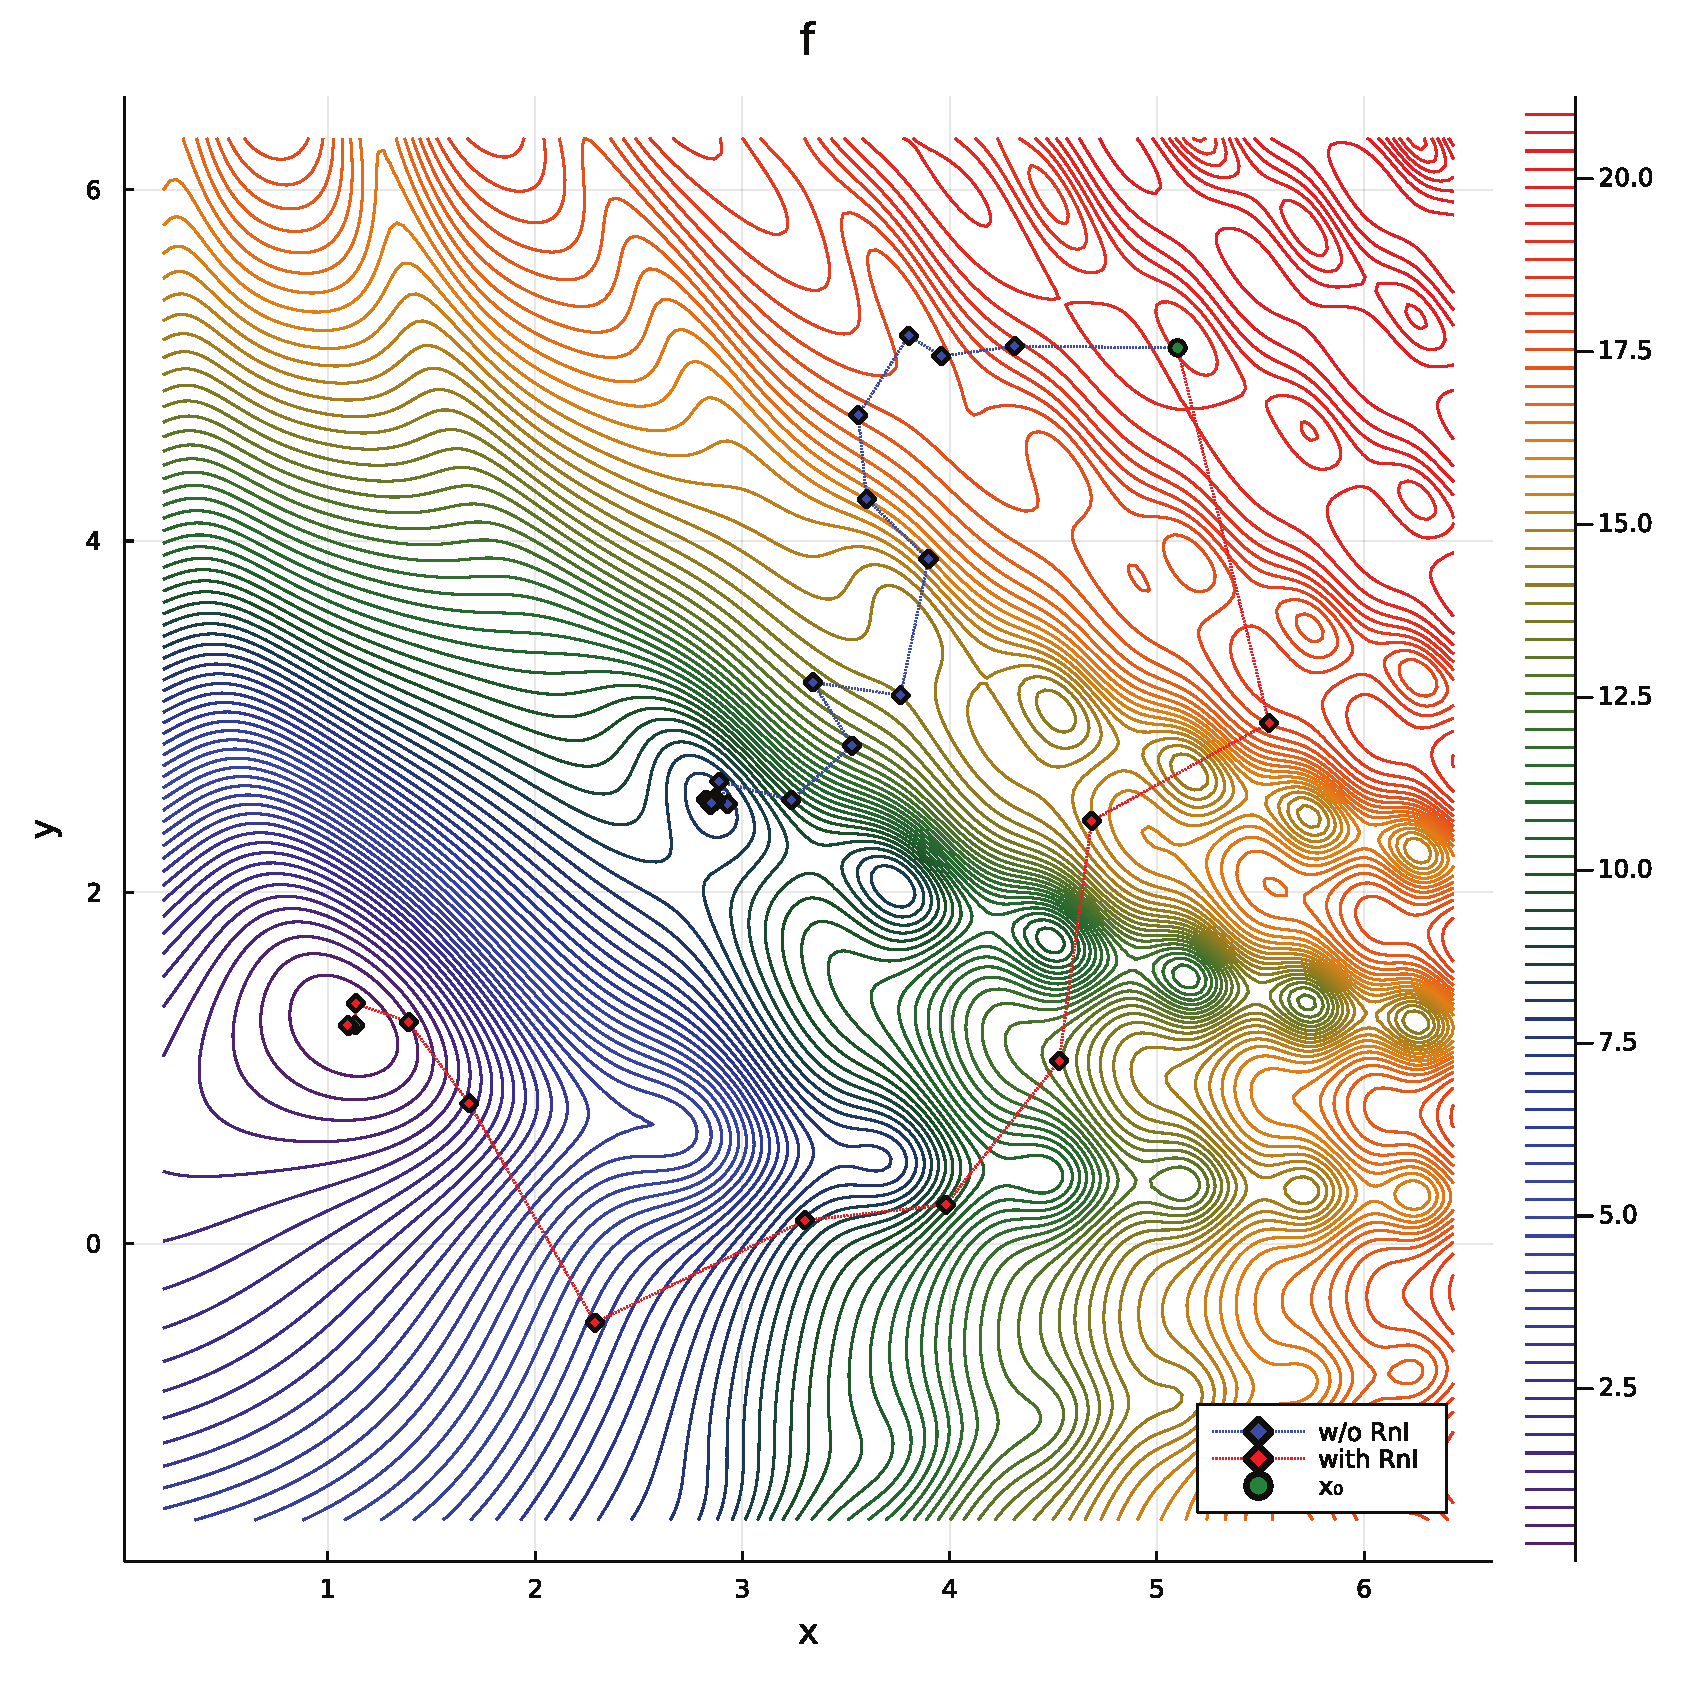
\includegraphics[width=0.7\linewidth]{asym_Ackley_sols.eps}}
    \caption{Comparison of CARS and the Inspect-as-Running version of CARS for the asymmetric Ackley function}
    \label{fig: Ackley asymmetric}
\end{figure*}

\subsection*{K-means Clustering}
Let $\{x_i\}_{i=1}^{n}$ be a set of $n$ points in $\mathbb{R}^d$ and $\{z_j\}_{j=1}^{K}$ be $K$ points in $\mathbb{R}^d$. Let the variable $Z = [z_1, \cdots, z_K] \in \mathbb{R}^{d \times K}$ be the matrix of the cluster centers. The K-means clustering problem is to find the optimal $Z$ that minimizes the following objective function:
\begin{equation*}
    f(Z) = \frac{1}{2n} \sum_{i=1}^{n} \min_{j=1,\cdots,K} \|x_i - z_j\|^2.
\end{equation*}
We tackle this problem with derivative-free methods by treating $Z$ as a vector in $\mathbb{R}^{dK}$.

\subsubsection*{Synthetic Gaussian data from \cite{yin2018stochastic}}
The first problem has synthetic Gaussian data, which is a mixture of four multivariate Gaussian distributions with $n = 1000$ each. This problem is introduced in \cite{yin2018stochastic}. We used the same means and covariance matrices:
\begin{align*}
    \mu_1 = [-5, -3], \mu_2 = [5, -3], \mu_3 = [0, 5], \mu_4 = [2.5, 4],
\end{align*}
    and 
\begin{align*}
    \Sigma_1 = \begin{bmatrix}
        0.8 & 0.1 \\ 0.1 & 0.8
    \end{bmatrix}, 
    \Sigma_2 = \begin{bmatrix}
        1.2 & 0.6 \\ 0.6 & 0.7
    \end{bmatrix}, 
    \Sigma_3 = \begin{bmatrix}
        0.5 & 0.05 \\ 0.05 && 1.6
    \end{bmatrix},
    \Sigma_4 = \begin{bmatrix}
        1.5 & 0.05 \\ 0.05 & 0.6
    \end{bmatrix}.
\end{align*}
\begin{figure*}
    \centering
    {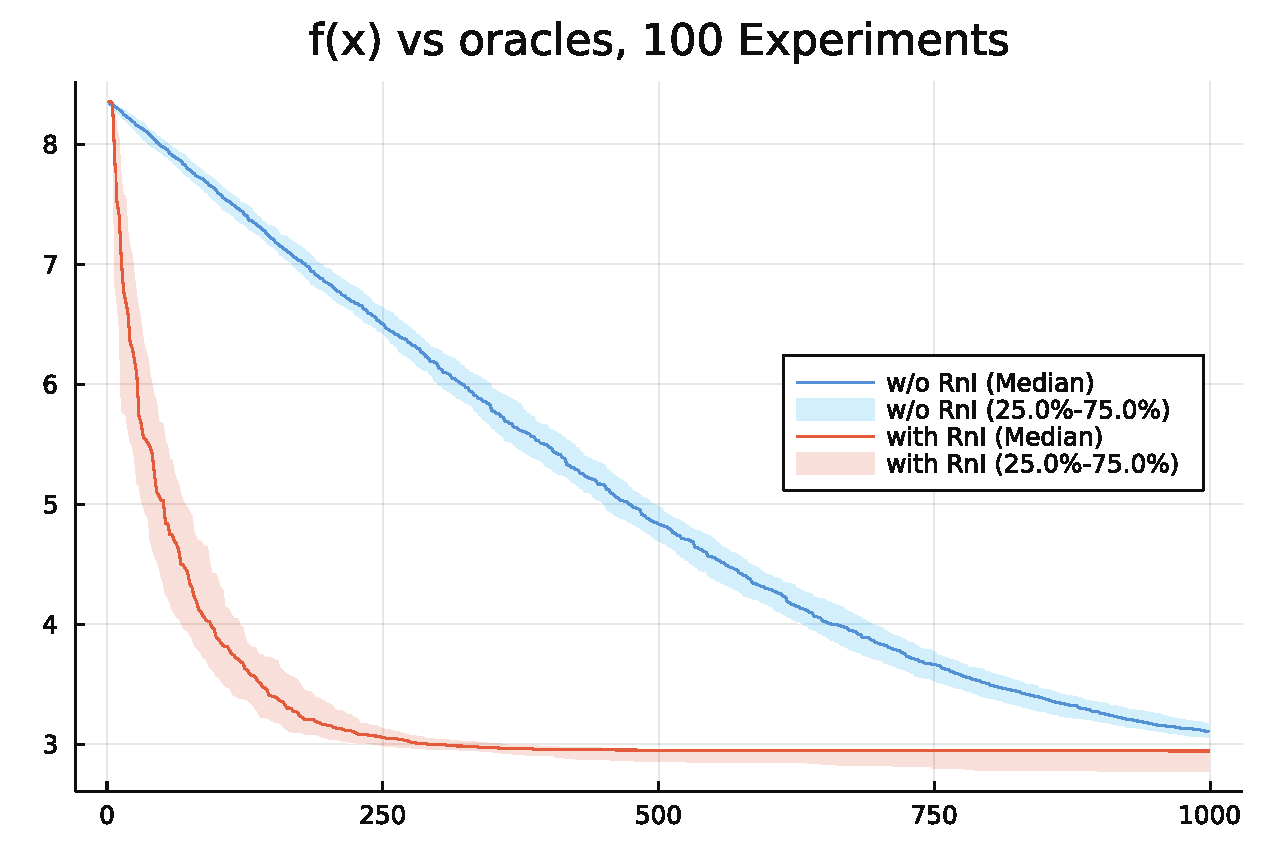
\includegraphics[width=0.7\linewidth]{Kmeans_h0_0.136.eps}}\\
    \vspace{3mm}
    {\includegraphics[width=0.7\linewidth]{Kmeans_h0_0.136_2dplot.eps}}
    \caption{Comparison of CARS and the Inspect-as-Running version of CARS for the K-means clustering problem of synthetic Gaussian data}
    \label{fig: K-means synthetic}
\end{figure*}

\subsubsection*{Iris data}
The second K-means clustering problem consists of the Iris dataset. This dataset contains 150 samples of three different species of Iris flowers. Each sample has four features: sepal length, sepal width, petal length, and petal width.
\begin{figure}
    \centering
    {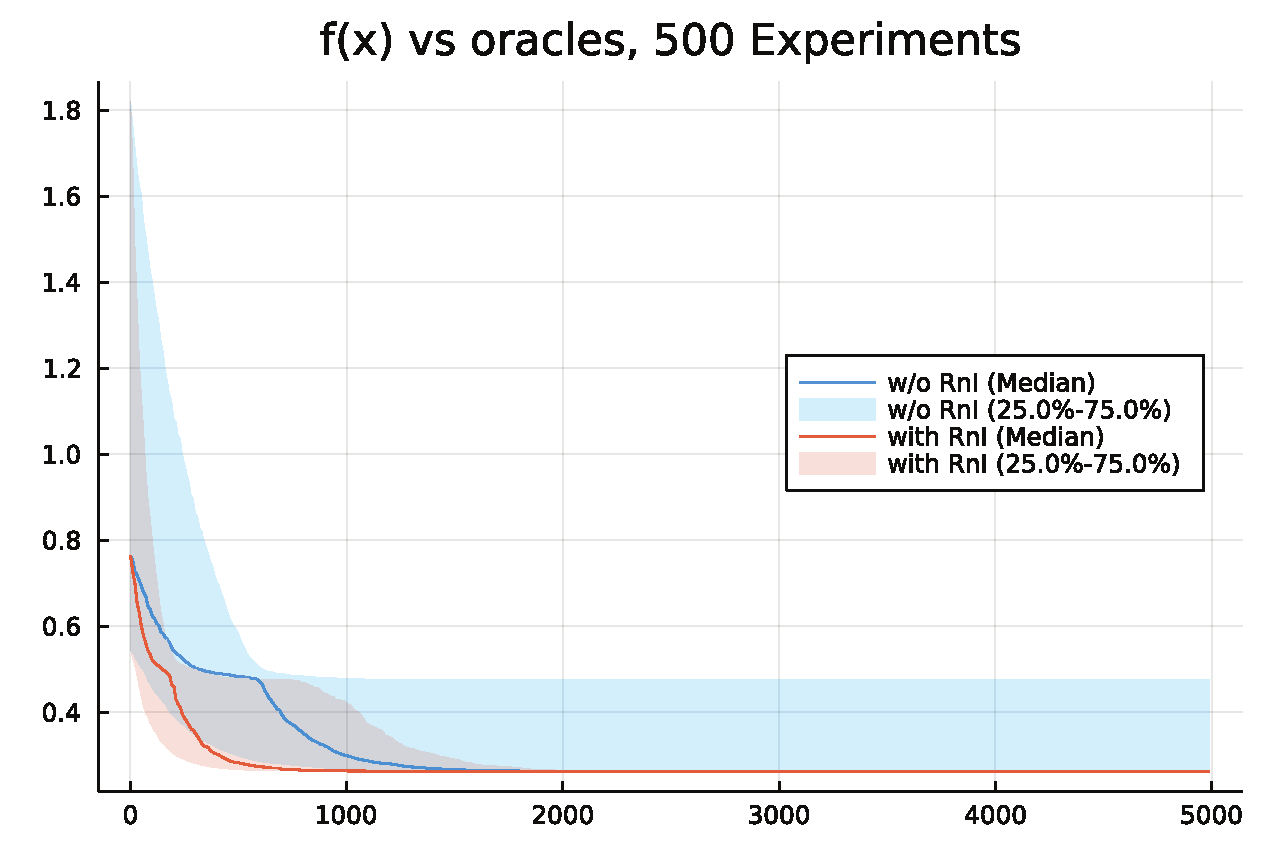
\includegraphics[width=0.7\linewidth]{Iris_h0_1.36e-3_R3.eps}}\\
    \vspace{3mm}
    {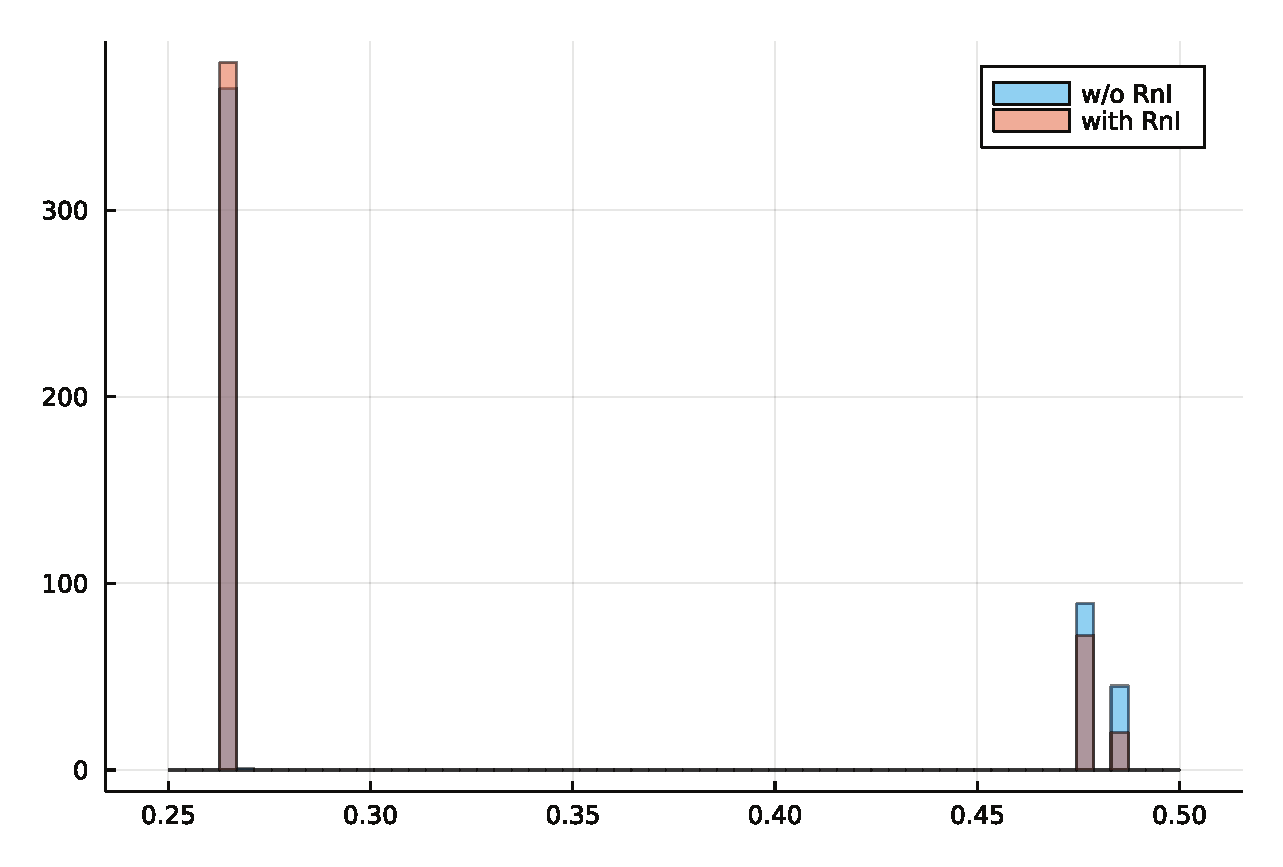
\includegraphics[width=0.7\linewidth]{Iris_histogram.eps}}
    \caption{Comparison of CARS and the Inspect-as-Running version of CARS for the K-means clustering of the Iris dataset}
    \label{fig: K-means Iris}
\end{figure}
We illustrate the results from 500 runs and the histogram of the final objective values in Figure~\ref{fig: K-means Iris}.
The figures demonstrate that the IR version of CARS finds better minima in most cases, and more rapidly.

\subsection*{Hyperparameter tuning}
We applied the two versions of CARS to hyperparameter tuning for training a convolutional neural network on the MNIST dataset.
The hyperparameters included the $L^2$ regularization parameter in the loss, the learning rate for the optimizer (AdaDelta), and the annealing rate for the scheduler (StepLR). To show the ability to escape the local minima more clearly, we started from a suboptimal initial point $x_0 = (0.5, 0.5, 0.5)$.

To reduce the variance, the objective function for the hyperparameter is set to be the mean of two samples, which measures the misclassification rate of the trained model with the given set of hyperparameters.

\begin{figure}
    \centering
    {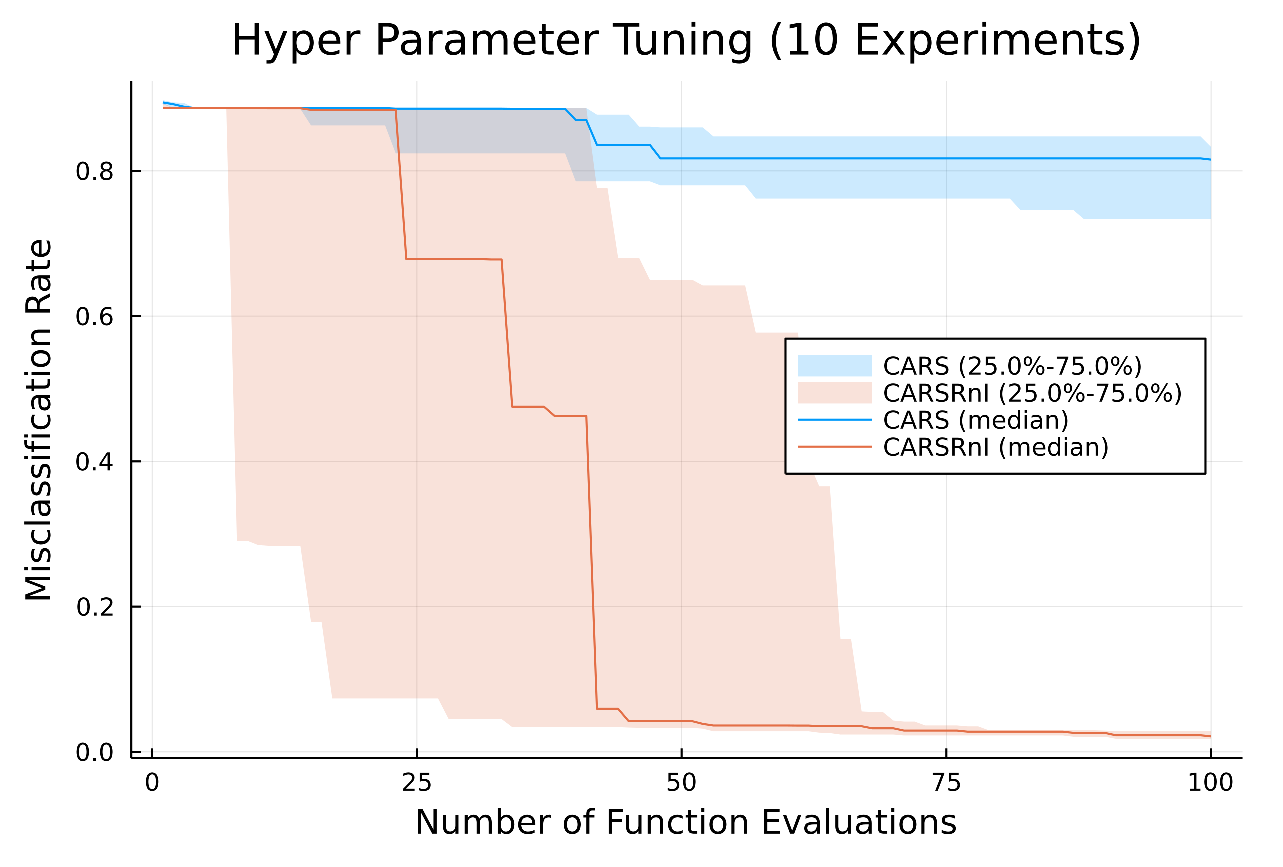
\includegraphics[width=0.7\linewidth]{CARS_vs_CARSRnI_julia.eps}}\\
    \vspace{3mm}
    {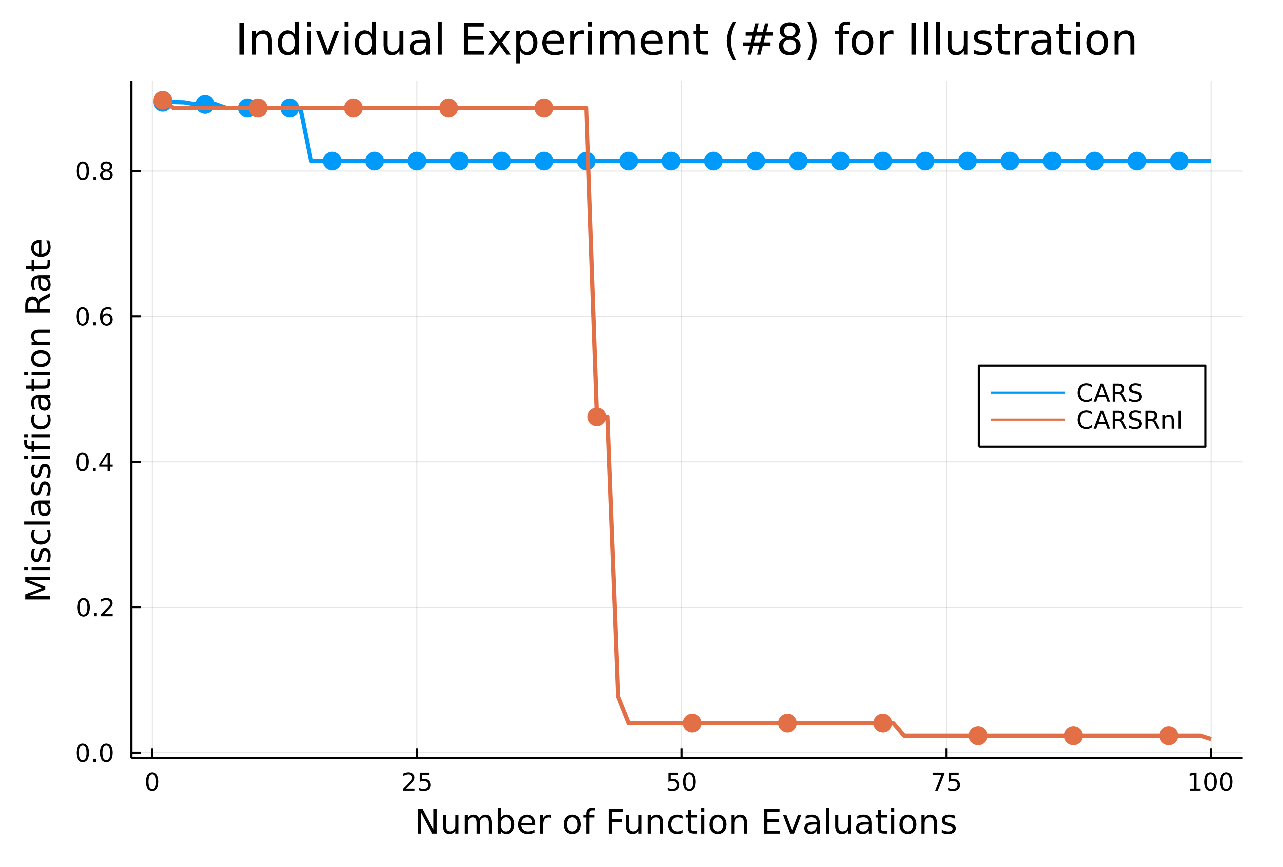
\includegraphics[width=0.7\linewidth]{CARS_vs_CARSRnI_Individual_julia.eps}}
    \caption{Comparison of CARS and the Inspect-as-Running version of CARS for hyperparameter tuning for training a convolutional neural network for MNIST dataset}
    \label{fig: HP Tuning - MNIST}
\end{figure}

\subsection*{Spurious local minima in higher dimension}
We revisit the function with spurious local minima in higher dimension, $d=300$, and compare the performance of CARS and the IR version of CARS with the global method RBFOpt \cite{costa2018rbfopt}, which is one of the most efficient the global methods.
RBFOpt took 15,073 seconds for 1,000 iterations (1,241 function evaluations), while CARS ran in 1.474 seconds for 30,000 function evaluations.
Here we see that the computational cost of the solver itself (sub-problems) is much higher in the global methods, often making it impractical for high-dimensional problems.
Furthermore, to utilize the structure of the problem, namely independence of each variable, we adopted the coordinate descent version, by simply replacing the sampling directions from $\unif(\mathbb{S}^{d-1})$ to $\unif(\{e_1, \cdots, e_d\})$, both for CARS and inspections.
\begin{figure}
    \centering
    {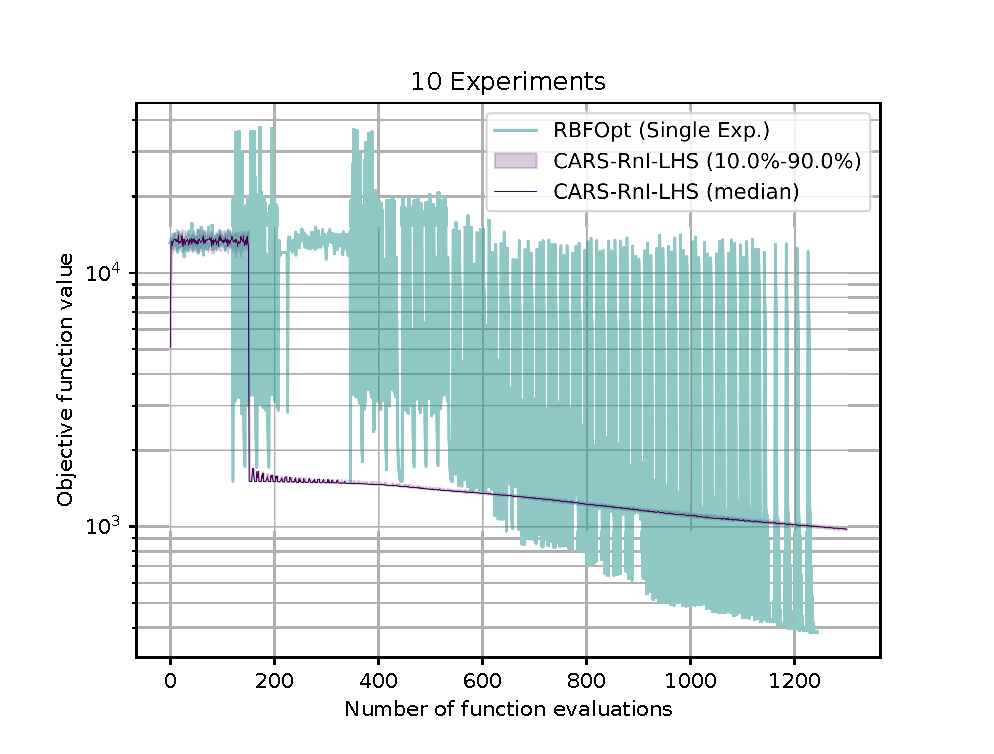
\includegraphics[width=0.7\linewidth]{X_small_300dim.eps}} \\
    \vspace{3mm}
    {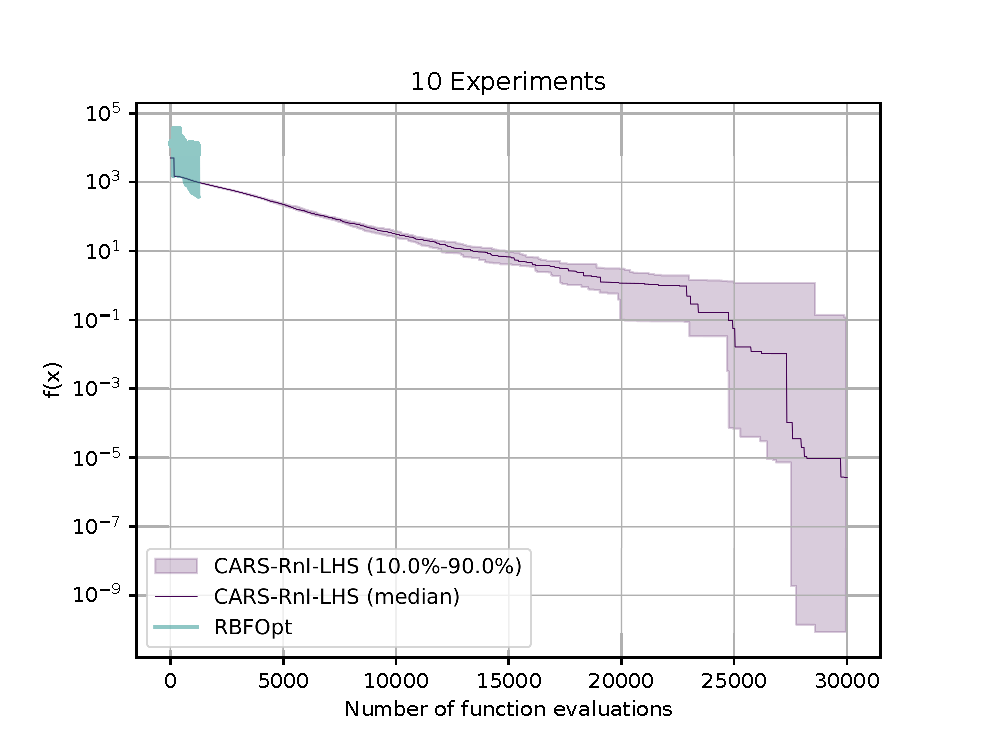
\includegraphics[width=0.7\linewidth]{X_all_300dim.eps}}
    \caption{Comparison of CARS with IR and the RBFOpt in 300-dimensional problem with spurious local minima. Computation for RBFOpt is terminated after 1,000 iterations due to the computational cost.}
\end{figure}




\chapter{Conclusion}
In this concluding chapter, we summarize the key findings of this thesis and suggest potential future research directions.

\section{Summary}
This thesis presents two novel approaches designed to enhance local Derivative-Free Optimization (DFO) methods, along with novel theoretical analyses and numerical experiments that underscore their efficacy.

In the first approach, we introduce a DFO method coined as Curvature-Aware Random Search (CARS), which leverages curvature information to optimize the step size along the search direction. We further refine CARS to develop the variants CARS-CR and CARS-NQ, creating a suite of lightweight, query-efficient DFO algorithms that can be easily implemented. 
Our analysis establishes the convergence on strongly convex functions for CARS and convex functions for CARS-CR. Specifically, we develop a novel and rigorous analysis on the finite difference errors and the probability of significant descents of the objective function. 
CARS-NQ utilizes Gauss-Hermite quadrature to more accurately estimate the directional derivatives, thereby improving robustness against highly oscillatory noise. 
The adaptability of the CARS family to various distributions enables their use in a wide range of problem-specific distributions. 
Furthermore, we present a novel randomized matrix inversion method that provides an unbiased estimator of an inverse matrix, computed via only quadratic measurements.
This is the cornerstone of Stochastic Hessian Inversion for Projected Search (SHIPS) approach for more curvature information, wherein quadratic measurements are estimated by finite differences.
 We demonstrate the efficacy of CARS and its variants through benchmark tests, where they outperform existing methods in minimizing non-convex functions as well.

In the subsequent chapter, we outline an inspection strategy for DFO methods, Inspect as you Run (IR), which can be applied to any DFO method that generates a sequence of iterates. Our analysis establishes a high probability guarantee for approximate $R$-local minima, without compromising the local convergence property of the original DFO method. Extensive benchmark tests have shown the exceptional effectiveness of the inspection strategy, affirming its ability to bridge the gap between local and global DFO methods.

\section{Future Research Directions}
\begin{itemize}
    \item \textbf{Variance Reduction} While the cost-effectiveness of sampling a single direction per iteration is beneficial, it does lead to a higher variance at each iteration.
    This challenge can be addressed by sampling multiple directions per iteration, as suggested in \cite{liu2020primer}.
    However, unlike DFO methods that mimic first-order methods, CARS involves a ratio of two estimators. The viewpoint introduced in Section~\ref{section: connection to ES} could provide useful insights into this issue and facilitate the multi-sample extension of CARS. Additionally, when a gradient estimate is available, combining it with finite difference estimates could further mitigate the variance.
    \item \textbf{Adaptive Sampling Distribution} We showed in Section~\ref{section: connection to ES} that CARS corresponds to an evolution strategy on the isometric population, solely shifting its mean. We also suggest updating the distribution's covariance \eqref{eq: ES covariance update}. This concept has strong ties to randomized matrix inversion and adaptive sampling, as demonstrated in Algorithm~\ref{alg:RandInv_AS}. Although the latter approach appears to be less competitive in higher dimensions at present, further exploration may yield improvements.
    \item \textbf{Use of Inspection Points} Inspection strategy proposed here, while fundamentally simple in its approach of selecting random points and comparing them to the current minimum, could potentially be enhanced by more intelligent utilization of the inspection point. One possibility is to treat the inspection points as a batch of random directions with a larger sampling radius. This multiscale strategy may be slightly more complex, but it has the potential to improve performance.
\end{itemize}

\appendix
\chapter{Appendix}
\section{Experimental Settings for Chapter~\ref{Chapter: CARS}}\label{appendix: Experiments}
In this Section, we list the hyperparameters we used for each experiment. The code for all experiments can be found in \url{https://github.com/bumsu-kim/CARS}. We ran experiments on several machines to distribute the load. We used Intel i5-9400F with Nvidia RTX 2060 and i9-9940X with two RTX 2080.

\paragraph{Mor\'{e}-Garbow-Hillstrom Problems.}
The Mor\'{e}-Garbow-Hillstrom Problem set consists of 34 non-convex smooth functions, where the problem dimension lies between 2 and 100. This experiment is conducted in Matlab.

We consider a problem solved when $f(x_k) - f_{\star} \leq \varepsilon(f(x_0) - f_\star)$. The target accuracies used here are $\varepsilon = 10^{-1}, 10^{-3}$ and $10^{-5}$.
We used the recommended $x_0$ for each problem.

For CARS and CARS-NQ, we used the sampling radius $r_k = 0.01/\sqrt{k+1}$, $\hat{L} = 2$. For CARS-NQ, the number of quadrature points $q=5$ is used. Having larger $q$ increases the accuracy of the approximation of smoothed derivatives, but it also increases the cost ({\em i.e.} function queries required) at each step. Recall from Section~\ref{section: CARS-NQ} that using odd $q$ is always more efficient than even $q$. Since $q=3$ is essentially less accurate than CARS, we used several values of $q\geq 5$ and found that $q=5$ is the best.

For STP \cite{bergou2020stochastic} and NSRS \cite{nesterov2017random} we used the same hyperparameters as given in Section 8.1 of \cite{bergou2020stochastic}. We also used the same decreasing step-size for Stochastic Momentum Three Points method (SMTP) \cite{gorbunov2019stochastic}. For the momentum parameter $\beta$ for SMTP, we followed \cite{gorbunov2019stochastic} and used $\beta = 0.5$.
Namely, following the notations in \cite{bergou2020stochastic} and \cite{gorbunov2019stochastic},
$\mathcal{D} = \unif {(\mathbb{S}^{d-1})}$ and 
\begin{align}
    \alpha_k & = \frac{1}{\sqrt{k+1}}, \tag{STP}\\
    \alpha_k & = \frac{1}{4(n+4)} \textrm{ and } \mu_k = 10^{-4}, \tag{NSRS}\\
    \gamma_k & = \frac{1}{\sqrt{k+1}}, \textrm{ and } \beta = 0.5. \tag{SMTP}
\end{align}

For SPSA \cite{spall1992multivariate} and 2SPSA \cite{spall2000adaptive}, we used the Rademacher distribution ({\em i.e.} $(u_k)_i = \pm 1$ with probability 0.5) for $\mathcal{D}$,  $\alpha = 0.602$, $\gamma = 0.101$, $A = 100$, $a = 0.16$, and $c = 10^{-4}$.

For AdaDGS \cite{tran2020adadgs}, we used the code provided by the authors, by implementing the original Python code in Matlab. Some modifications on hyperparameters are made due to the difference in the scale of problem dimension, and the lack of domain width. First, the original AdaDGS code performs experiments on high dimensional problems  ({\em e.g.} $d=1000$), whereas $2\leq d \leq 100$ in this experiment. Also, the problems are unconstrained, and $\|x_0-x_{\star}\|$ varies from order of $10^0$ to $10^6$.
Thus we used the following modified hyperparameters (following the notation of \cite{tran2020adadgs}):
\begin{enumerate}
    \item The number of points used for line search $S = 100$, since the suggested value $0.05d(M-1)$ is too small for our experiments.
    \item The initial smoothing(sampling) radius $\sigma_0 = 10^{-2}$. We tested $\sigma_0 = 5, 1, 10^{-1}, 10^{-2}$ and $10^{-3}$ and chose the best value. When $\sigma_0 \leq 10^{-1}$ then the results were similar.
\end{enumerate}

For plotting the performance profile, we set the performance ratio $r_{p,s} = r_{M}$ when $p$ is not solved by $s$. Having $r_M = \infty$ is ideal, but setting it by a sufficiently large number does not make any difference. We used $r_M = 10^{20}$.

\paragraph{Problems with Highly Oscillatory Noise.}
For the presence of oscillatory noise scenario, we performed experiments, by adding the noise to Mor\'{e}-Garbow-Hillstrom Problems.
For each function in the benchmark set, we used the same noise
\begin{equation*}
    f_{\mathrm{osc}}(x) = \psi \sum_{i=1}^{d}(1-\cos(\phi_i x_i)), 
\end{equation*}
with different noise level $\psi = 0.1\varepsilon(f(x_0)-f_\star)$, and the same frequency $\phi_i = 100\pi$.

We used the same hyperparameters for Mor\'{e}-Garbow-Hillstrom Problems as in the previous experiment, except for CARS-NQ, where we used 50 times larger $r$.

\paragraph{Black-box Adversarial Attacks.}
In this section, we explain the experiment setting for black-box adversarial attacks and also provide the hyperparameters that we used.
The CNN model we attack has two $5\times5$ convolutional layers with 6 and 16 output channels, followed by a $4\times 4$ convolutional layer with 120 output channels. Then two fully connected layers with 84 and 10 units follows. Between layers we use ReLU, and between convolutional layers we use $2\times 2$ max-pooling as well. Finally we apply log softmax to the output layer.
The test accuracy of the trained model is 98.99\%.

For more readable description, let the images have width and height both equal to $s$. Then the problem dimension $d$ is $s^2$. For this particular experiment, we make three modifications to CARS.
First, since the problem is highly non-convex ($h_r<0$ at around 50\% of the iteration), we don't compute $x_{\mathrm{CARS}}$ when $h_r < 0$ at $k$-th iteration.
The second modification is due to the constraint of the problem. Let $\mathcal{F}$ be the feasible set:
\begin{equation*}
    \mathcal{F} = \{x \in [0,1]^d : \|x-x_0\| \leq \varepsilon_{\mathrm{atk}} \}.
\end{equation*}
Inspired by \cite{andriushchenko2020square}, we also compute $x_{\mathrm{bdry}} = x_k - t_{\mathrm{max}}d_r u_k$, where
\begin{equation*}
    t_{\mathrm{max}} = \max \{ t > 0 : x_k - td_r u_k \in \mathcal{F}\}.
\end{equation*}
This is especially useful when $h_r < 0$ so we don't compute $x_{\mathrm{CARS}}$.
Therefore, CARS now requires either 3 ($f(x_k \pm r_k u_k)$ and $f(x_{\mathrm{bdry}})$) function queries or 
4 ($f(x_{\mathrm{CARS}})$ in addition) per iteration. To sum up,
\begin{align*}
    x_{k+1} = 
    \begin{cases}
        \argmin\{f(x_k \pm r_k u_k), f(x_{\mathrm{CARS}}), (x_{\mathrm{bdry}}) \} & \textrm{ if } h_r>0 \\
        \argmin\{f(x_k \pm r_k u_k), (x_{\mathrm{bdry}}) \} & \text{ otherwise. }
    \end{cases}
\end{align*}
Lastly, we perturbed $x_0$ by adding horizontal stripes. That is,
\begin{equation*}
    x_0 = \mathrm{proj}_{\mathcal{F}} (x_{\mathrm{orig}} + \varepsilon_{\mathrm{atk}} v),
\end{equation*}
where $v_{i,:} = \pm (1,\cdots,1)$ for $i=1,\cdots,s$ and $x_{\mathrm{orig}}$ is the image to be attacked. This choice of initialization is found to be very effective in \cite{andriushchenko2020square}.

We use the same sampling distribution as Square Attack \cite{andriushchenko2020square}, which is known to be particularly well-suited for attacking CNN models. Identifying $s\times s$ images and $d$-vectors,
this distribution generates a square block of all $1$ or $-1$, {\em i.e.} $u_{r+1:r+w, c+1:c+w} = \pm 1$, where $0 \leq r, c \leq s-w$ and $w$ is the window size. See \cite{andriushchenko2020square} for more details.

The window size $w$ is determined by $p$, the fraction of the pixels changed by attack. Namely, $w$ is the closest positive integer to $\sqrt{p}s$, and thus this $p$ is an important hyperparameter in this distribution.
In \cite{andriushchenko2020square}, the authors used $p = 0.8$ in the initial stage and halve the value of $p$ when the number of iteration $k$ reaches $10, 50, 200, 1000, 2000, 4000, 6000$ and $8000$, respectively.

For CARS, we used the initial $p=0.2$ and halved it at $k = 2, 10, 40, 250, 500, 800, 1200$ and $1600$. Note that the Square Attack only uses one function query at each iteration and CARS for black-box attack uses 3 or 4 queries, and thus $p$ is being halved at similar stage of the algorithms, in terms of the function queries.

Finally, the sampling radius $r_k$ is fixed by 1 for every iteration.

\section{Visualization of Attacked Images}
In this section we present the visualization of the attacked images, comparing them with the original images.
To be more clear, the images in Figure~\ref{fig:MNIST_ATK_RES_ALL} have {\em Testset ID} (TID)'s from 100 to 109.
When an image with label $n$ has TID $t$, this means it is the $t$-th $n$ appearing in the test set. See the code for more details on TID.
\begin{figure}[t]
    \centering
    \includegraphics[width=0.60\linewidth]{fig/fig_CARS/MNISTatk_imgs.png}
    \caption{Adversarial examples with misclassified labels on MNIST generated with CARS. For every two rows, a row of original images are shown, and the adversarial examples are right underneath them, with the misclassified labels in between.}
    \label{fig:MNIST_ATK_RES_ALL}
\end{figure}


%\bibliography {bib/network,bib/naming}    % bibliography references
\bibliographystyle{uclathes}                % see thesis.bst for details
\bibliography{realbib}

\end {document}

